\chapter{Results}\label{Chapter:Results}
\noindent

Make table of cross sections, one for each. 

\section{Iridium cross sections}


\begin{figure}%
    \centering
    \subfloat[]{{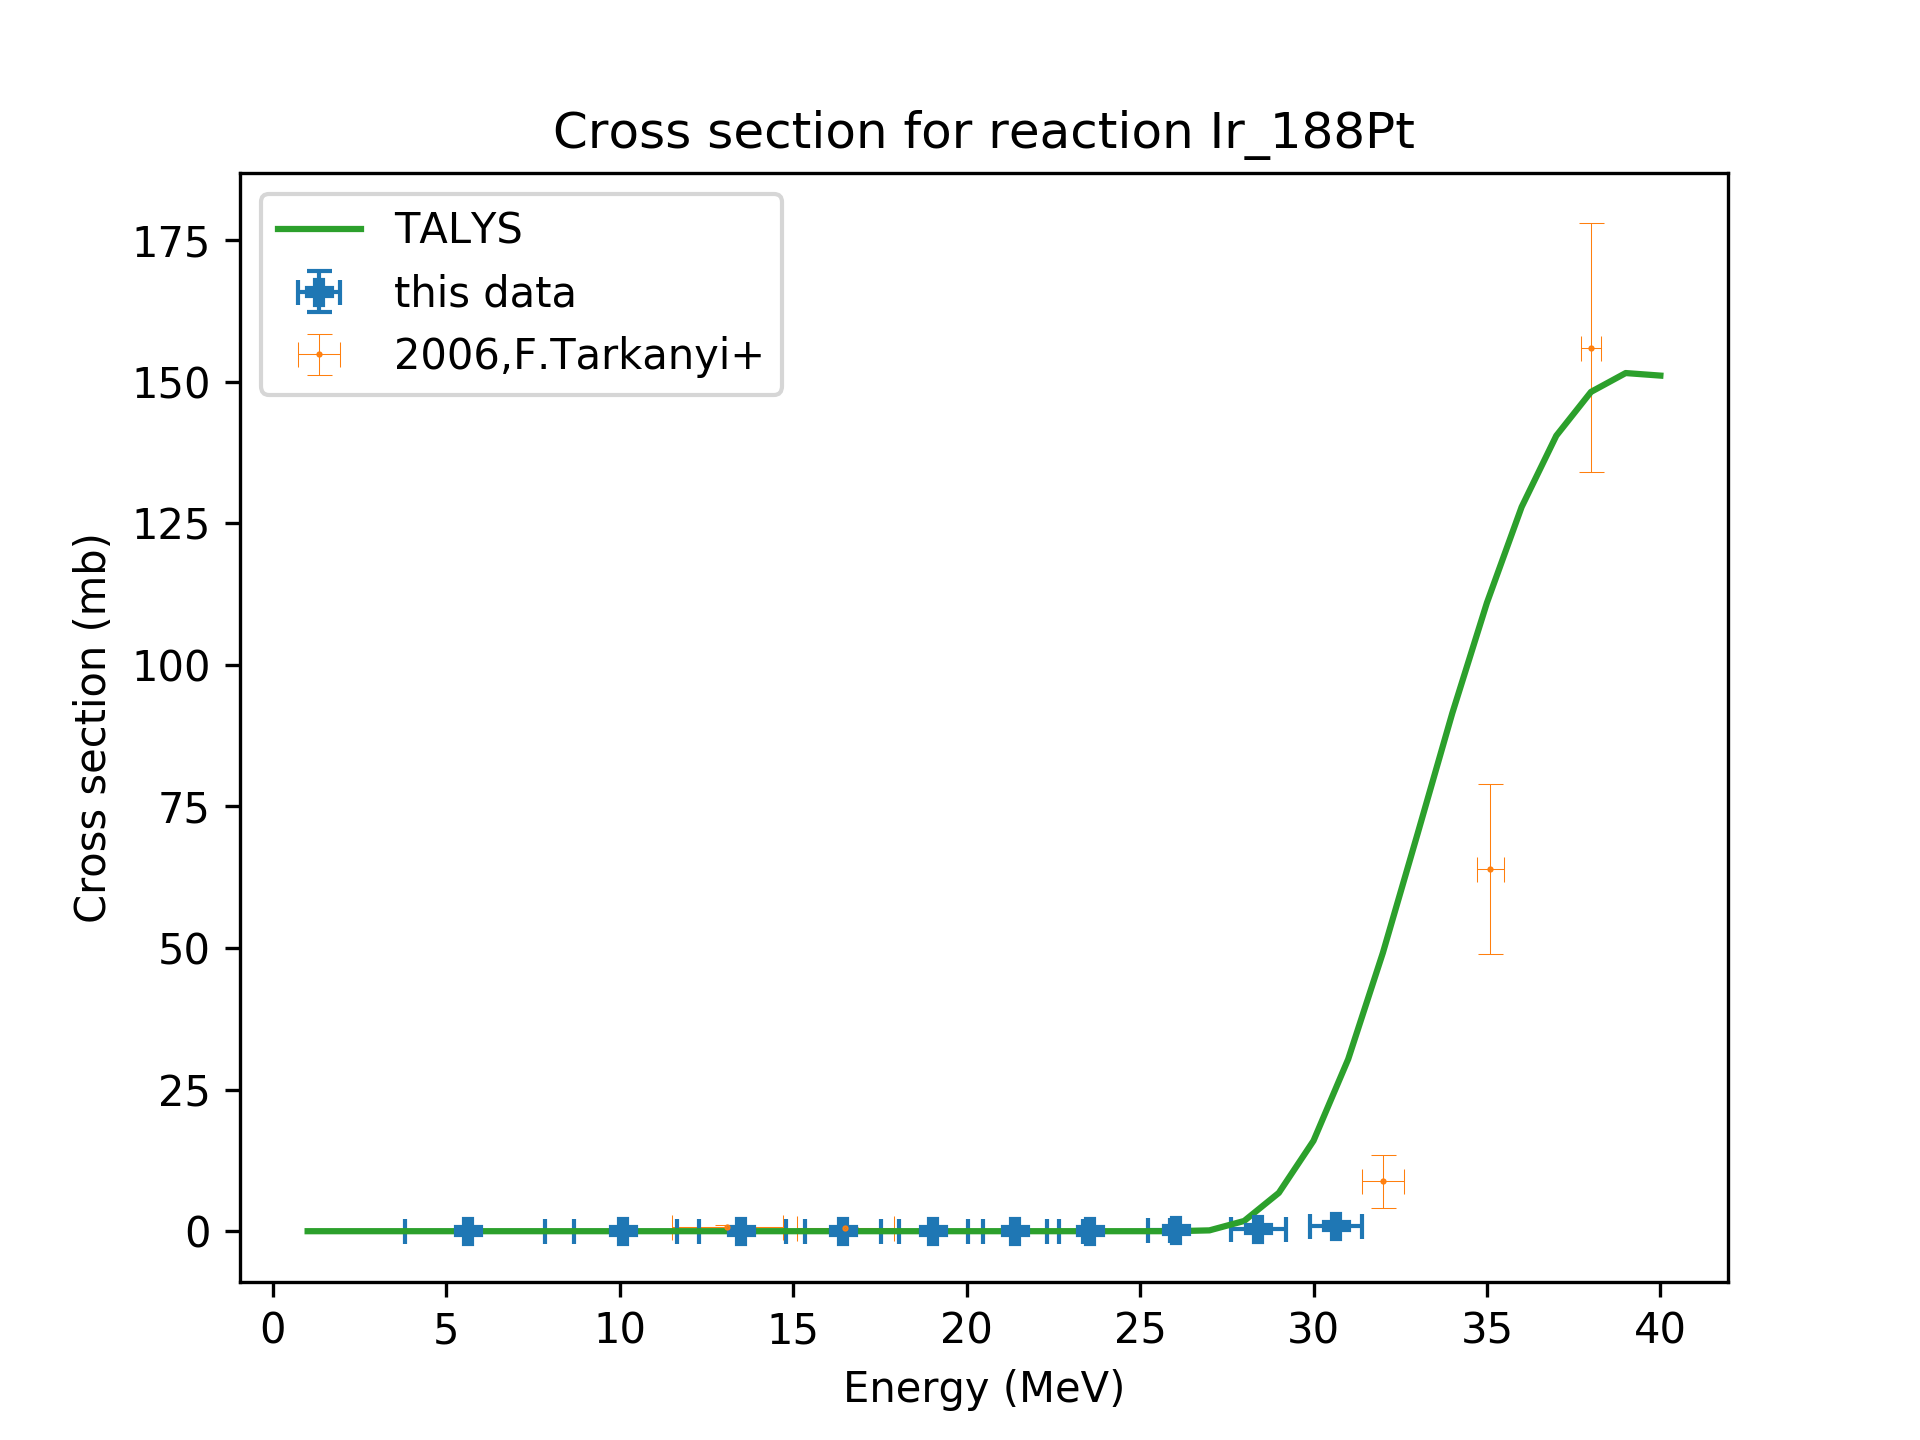
\includegraphics[width=5cm]{Results/Ir_188Pt.png}}%
    \quad
    \subfloat[]{{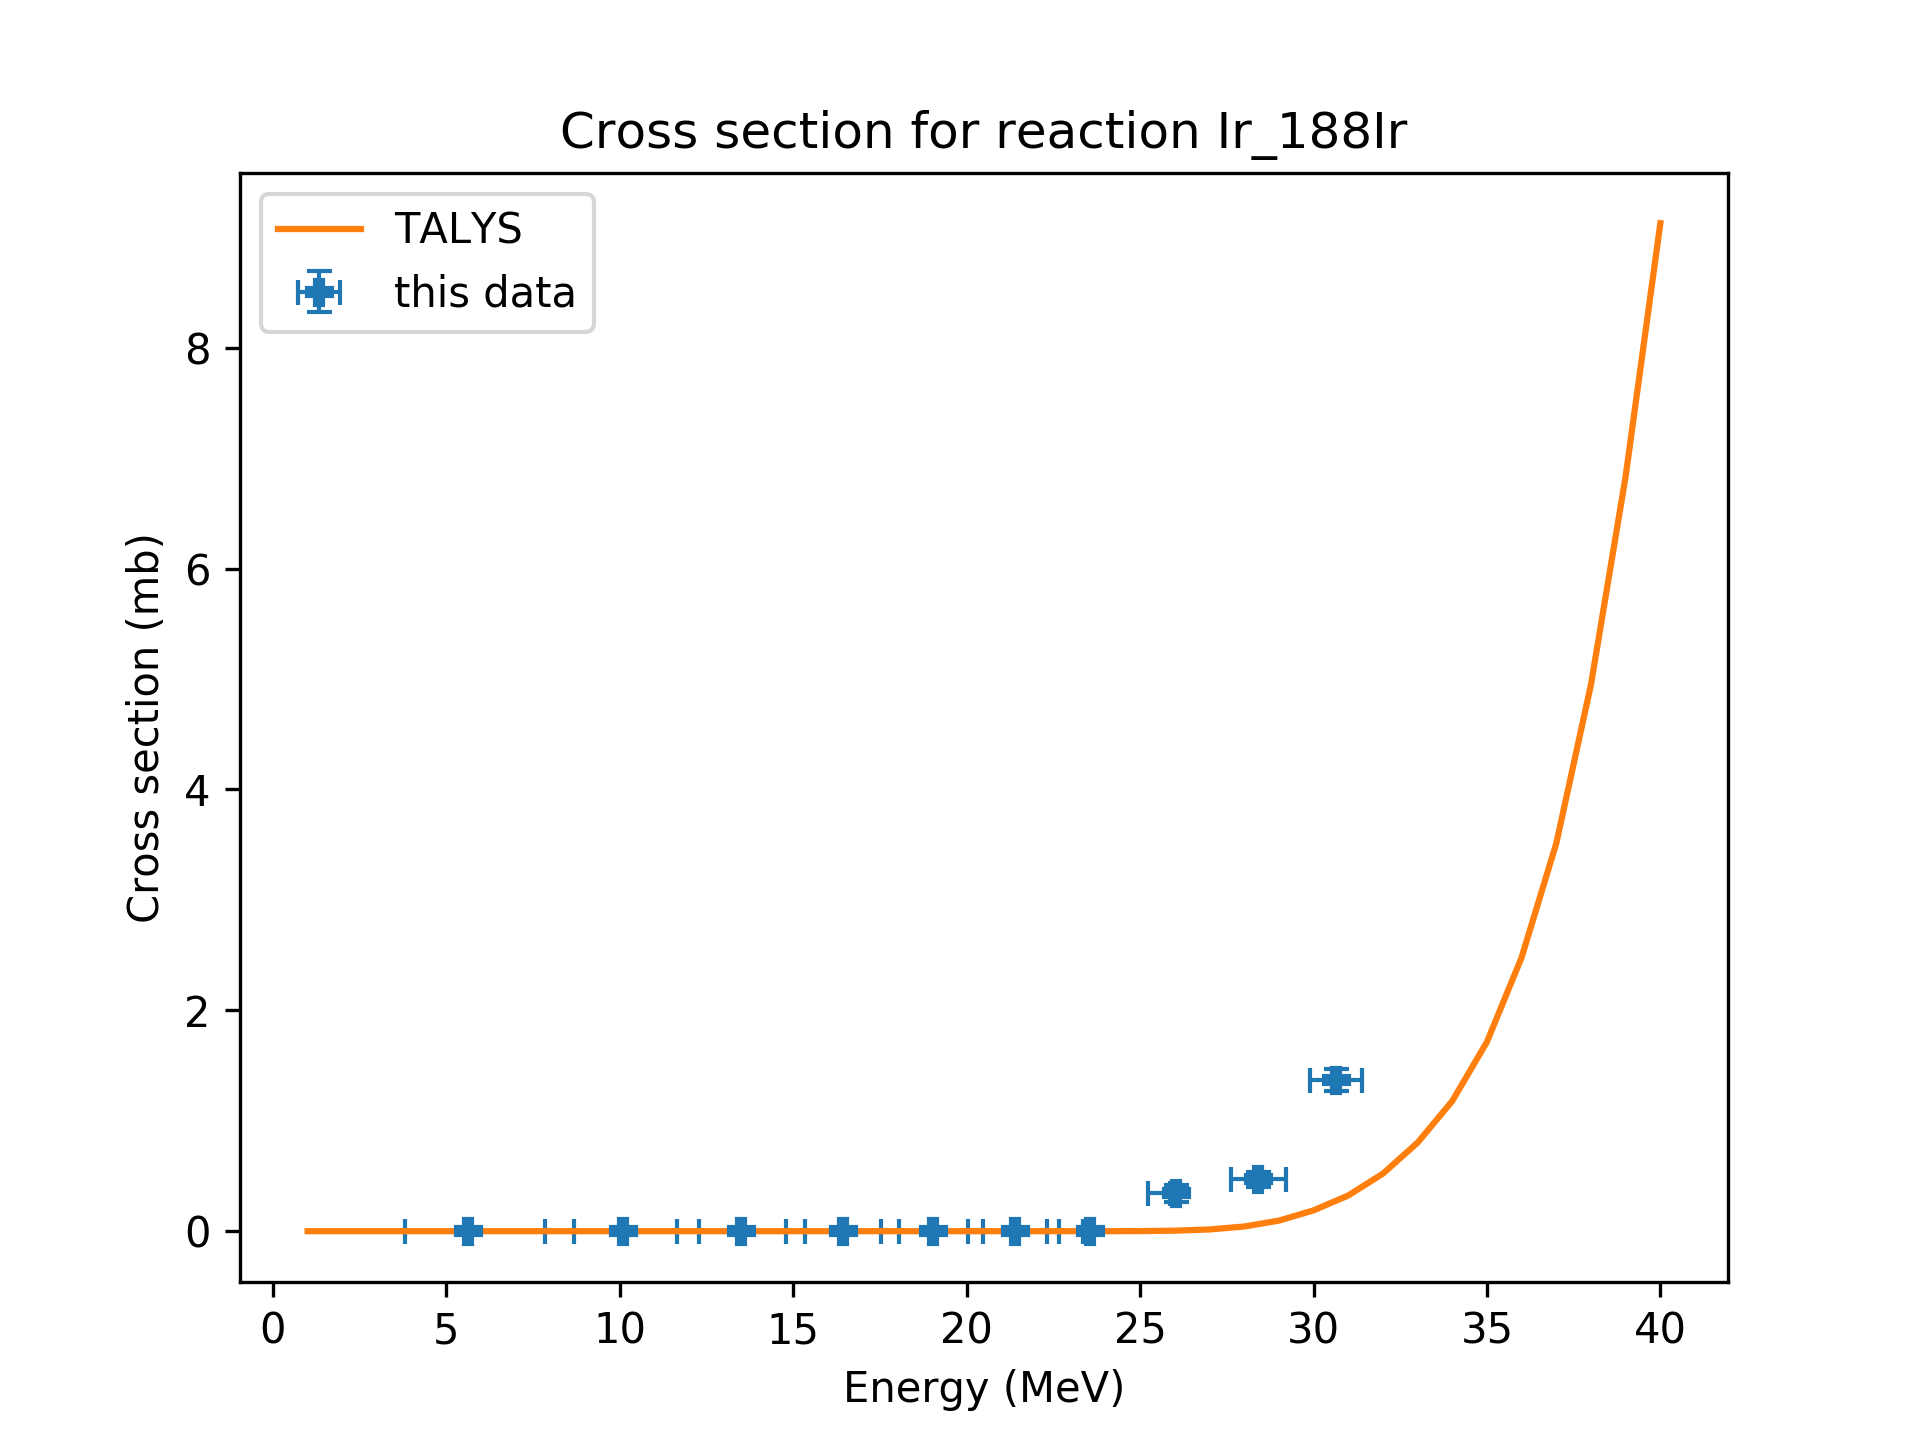
\includegraphics[width=5cm]{Results/Ir_188Ir.png} }}%
    \subfloat[]{{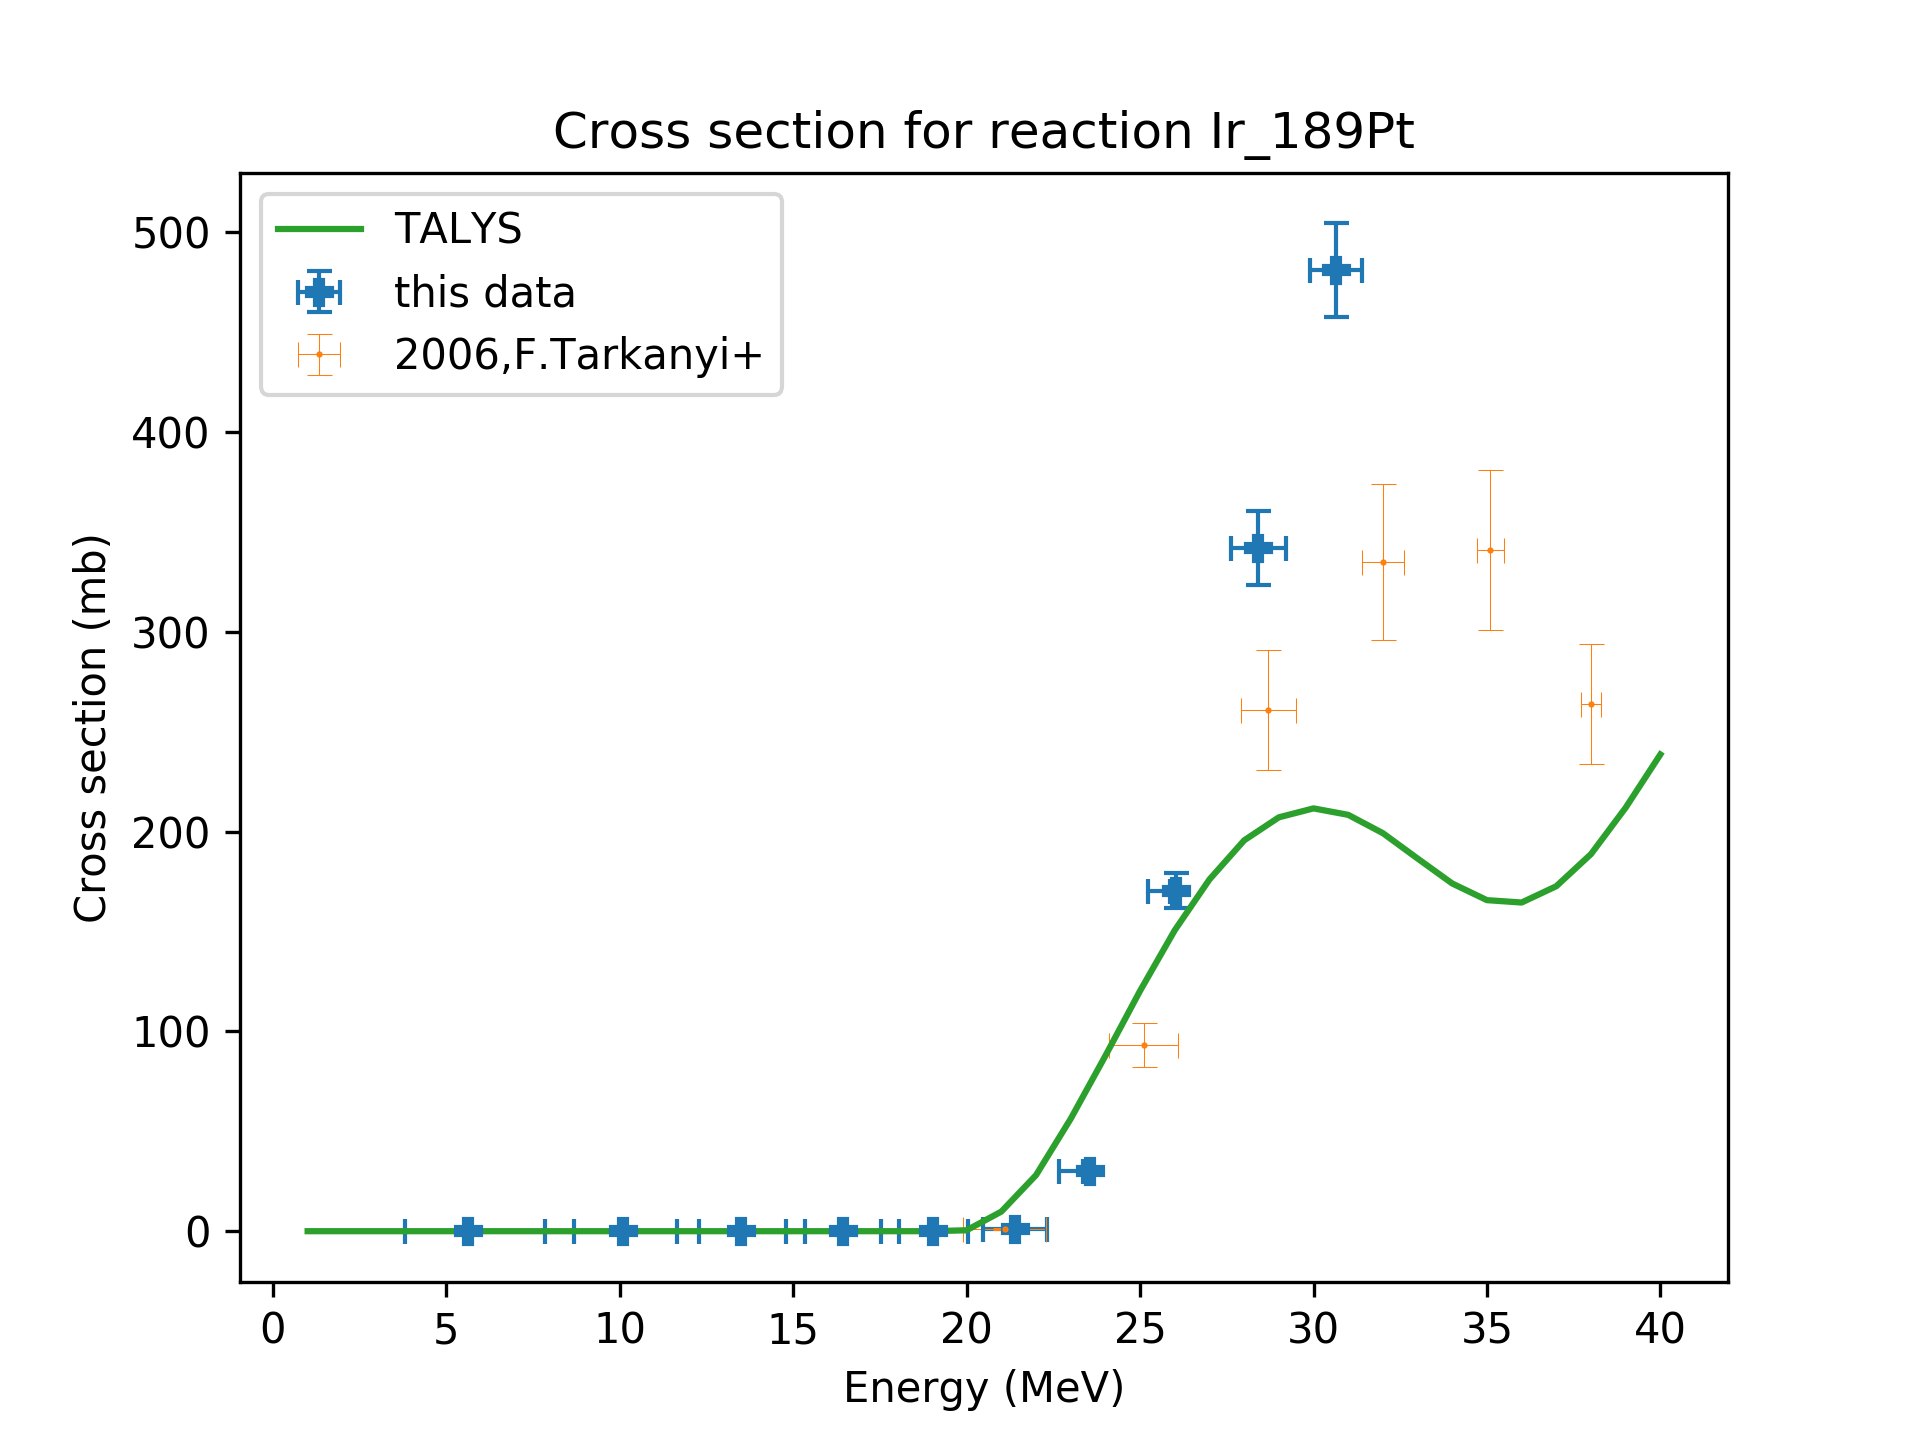
\includegraphics[width=5cm]{Results/Ir_189Pt.png} }}%
    \quad
    \subfloat[]{{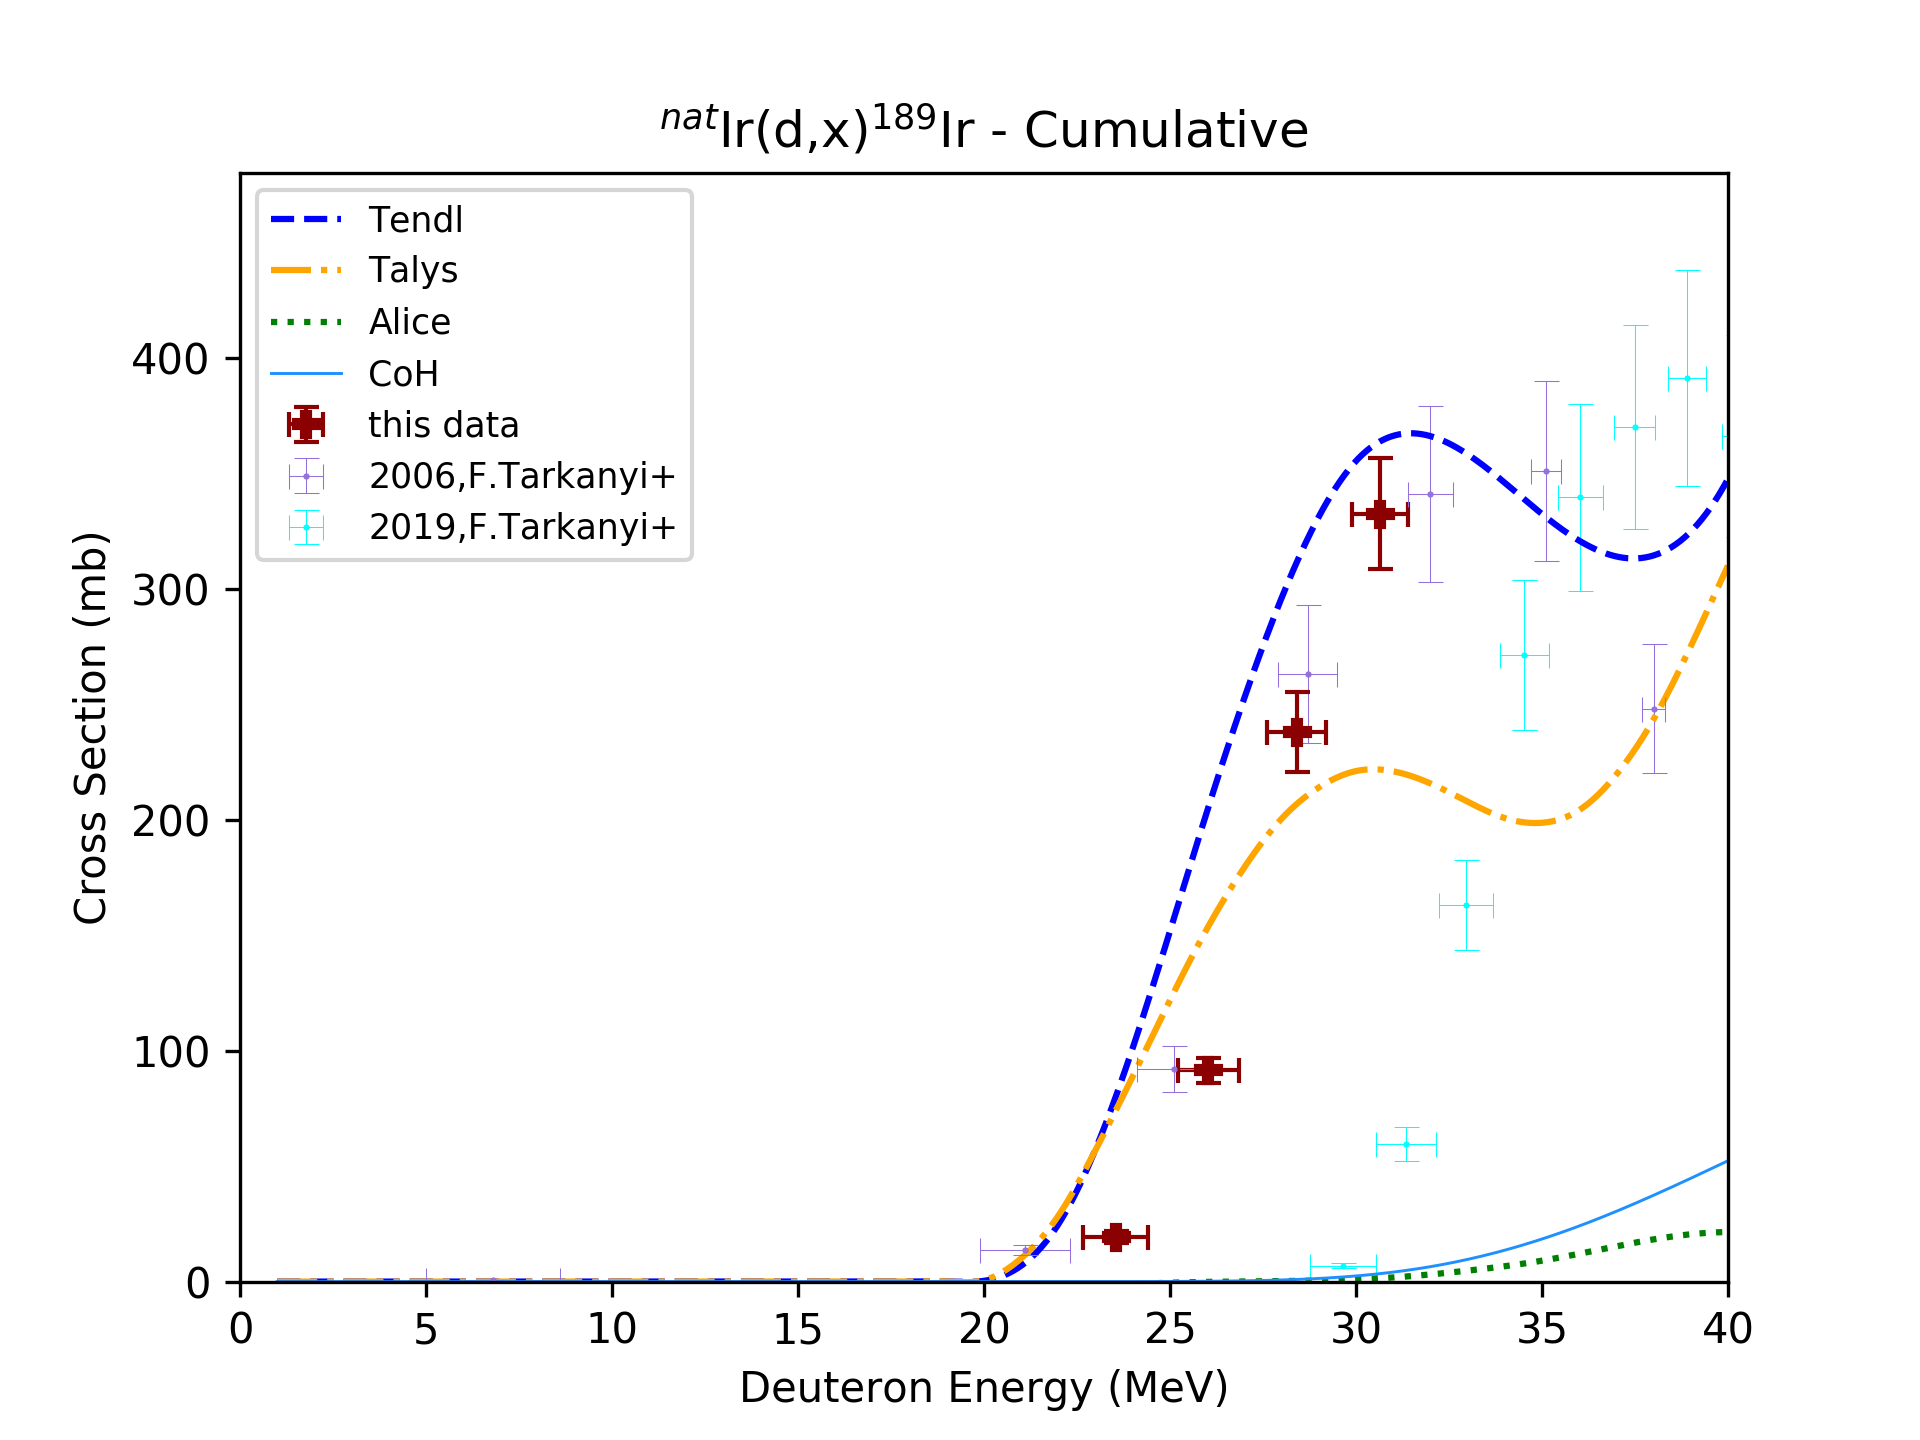
\includegraphics[width=5cm]{Results/Ir_189Ir.png} }}%
    \quad
    \subfloat[]{{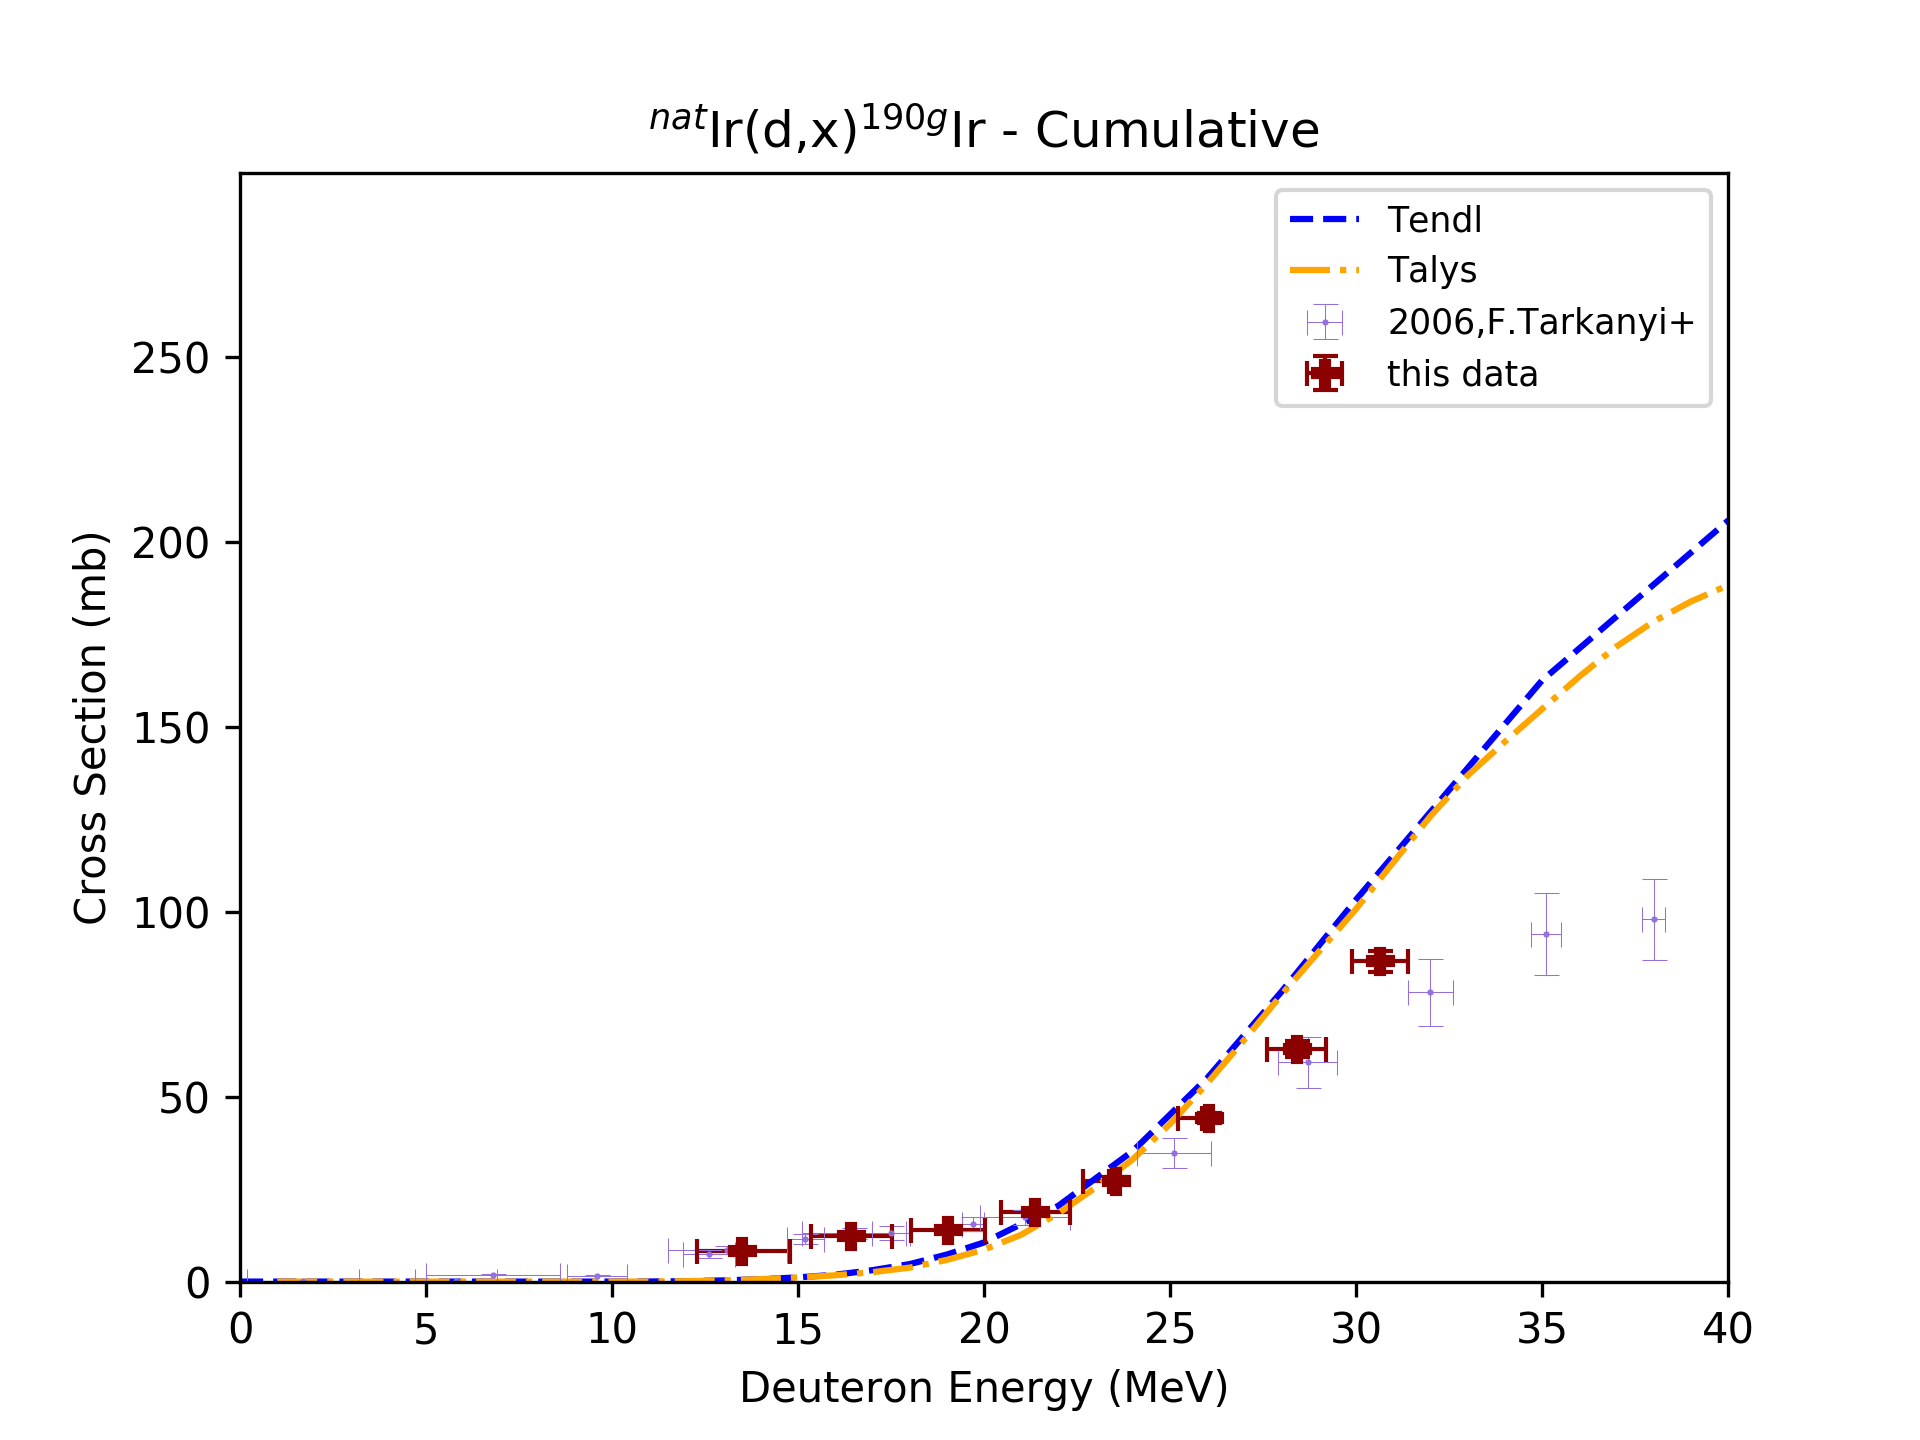
\includegraphics[width=5cm]{Results/Ir_190Ir.png} }}%
    \quad
    \subfloat[caption]{{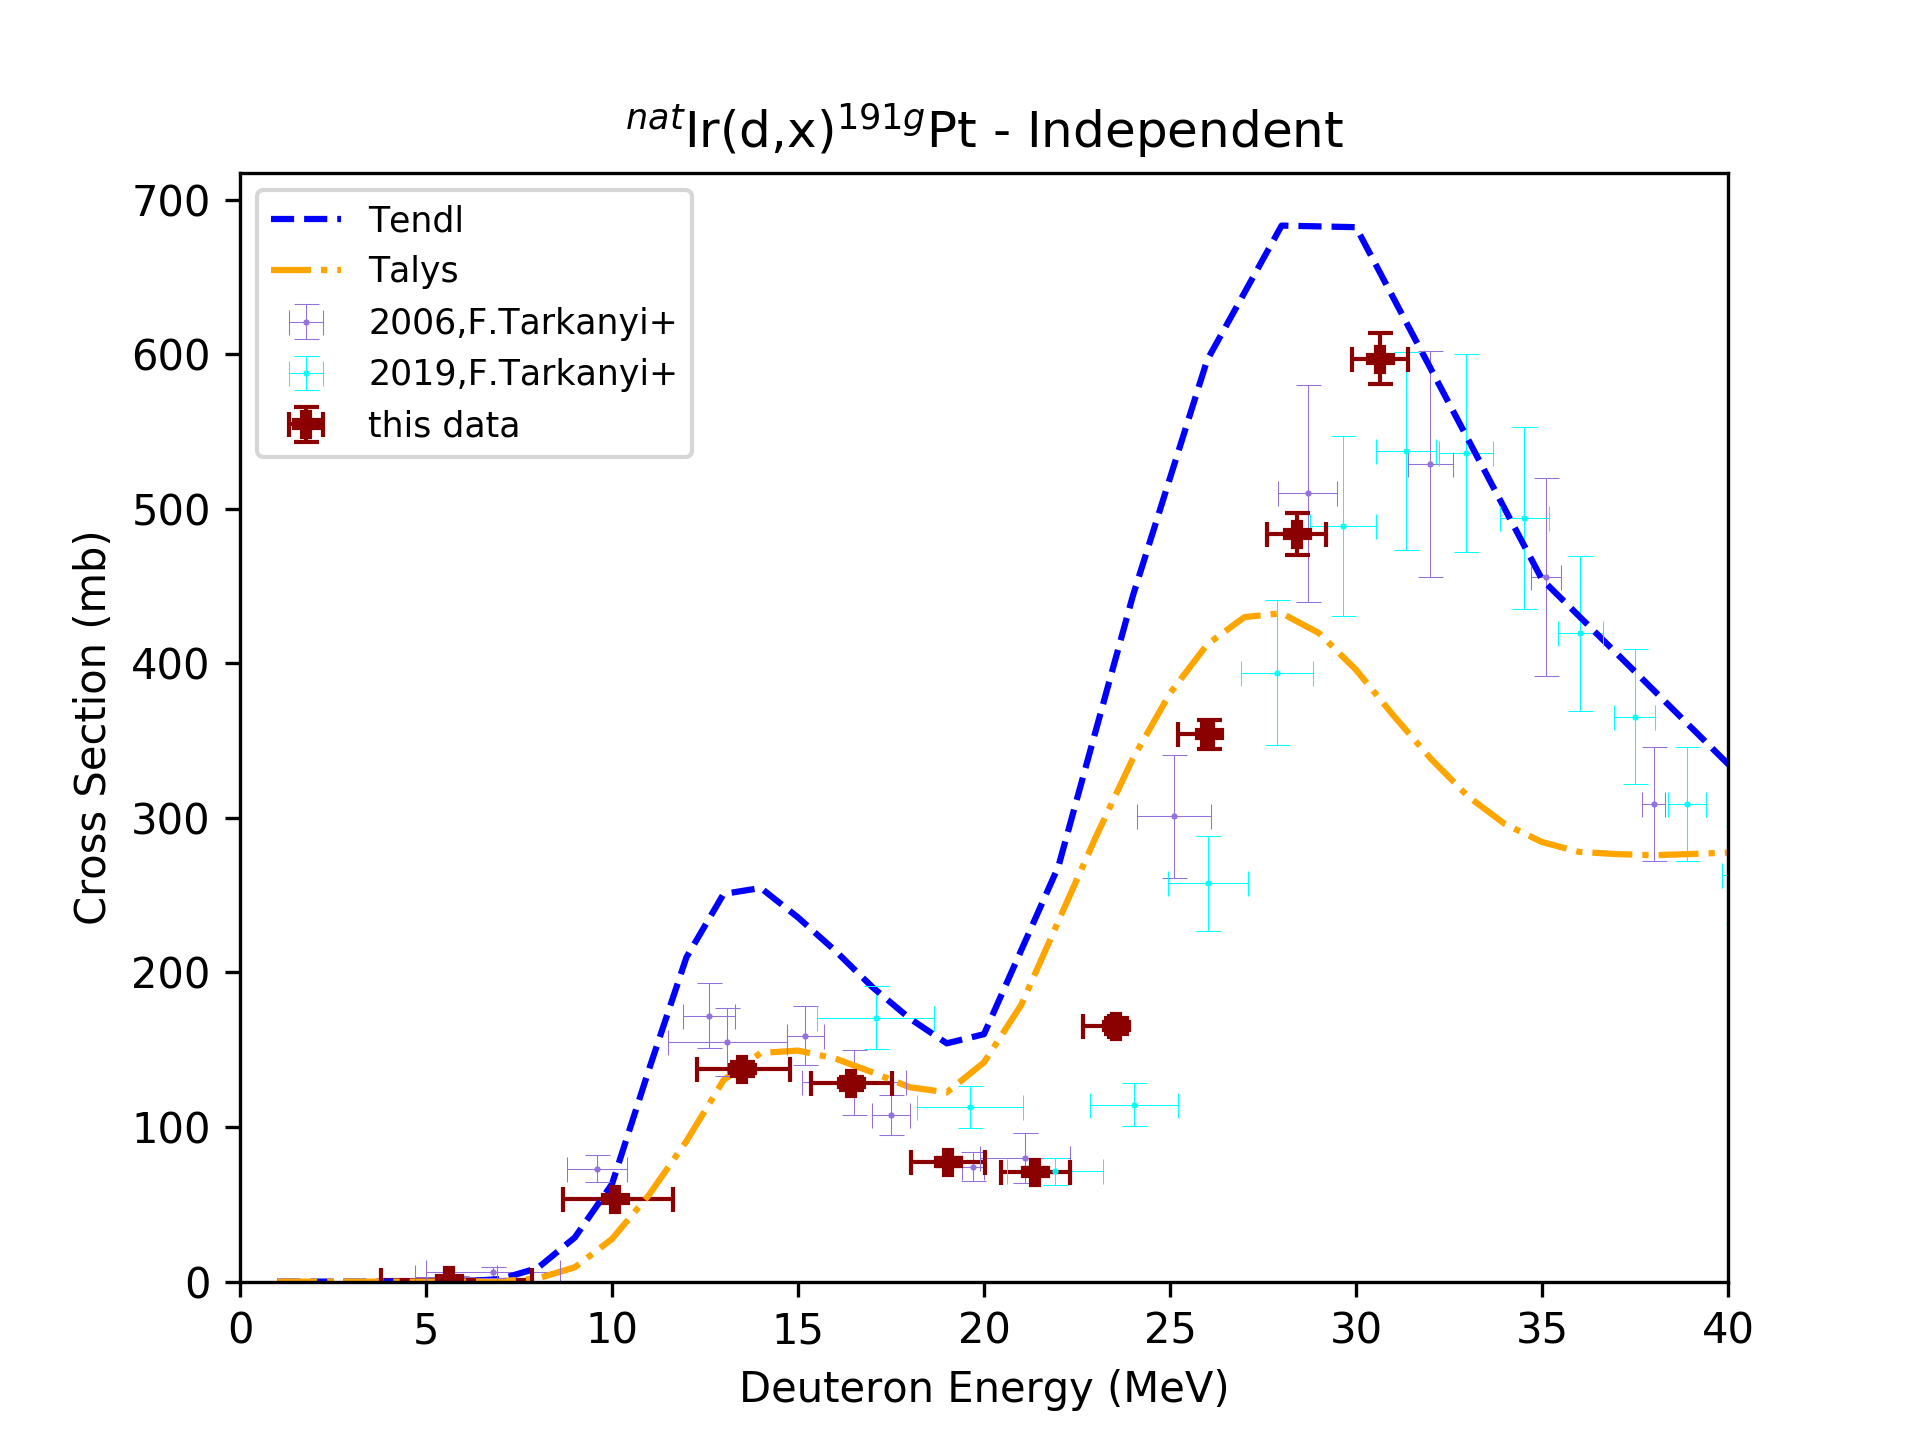
\includegraphics[width=5cm]{Results/Ir_191Pt.png} }}%
    \quad
    \subfloat[]{{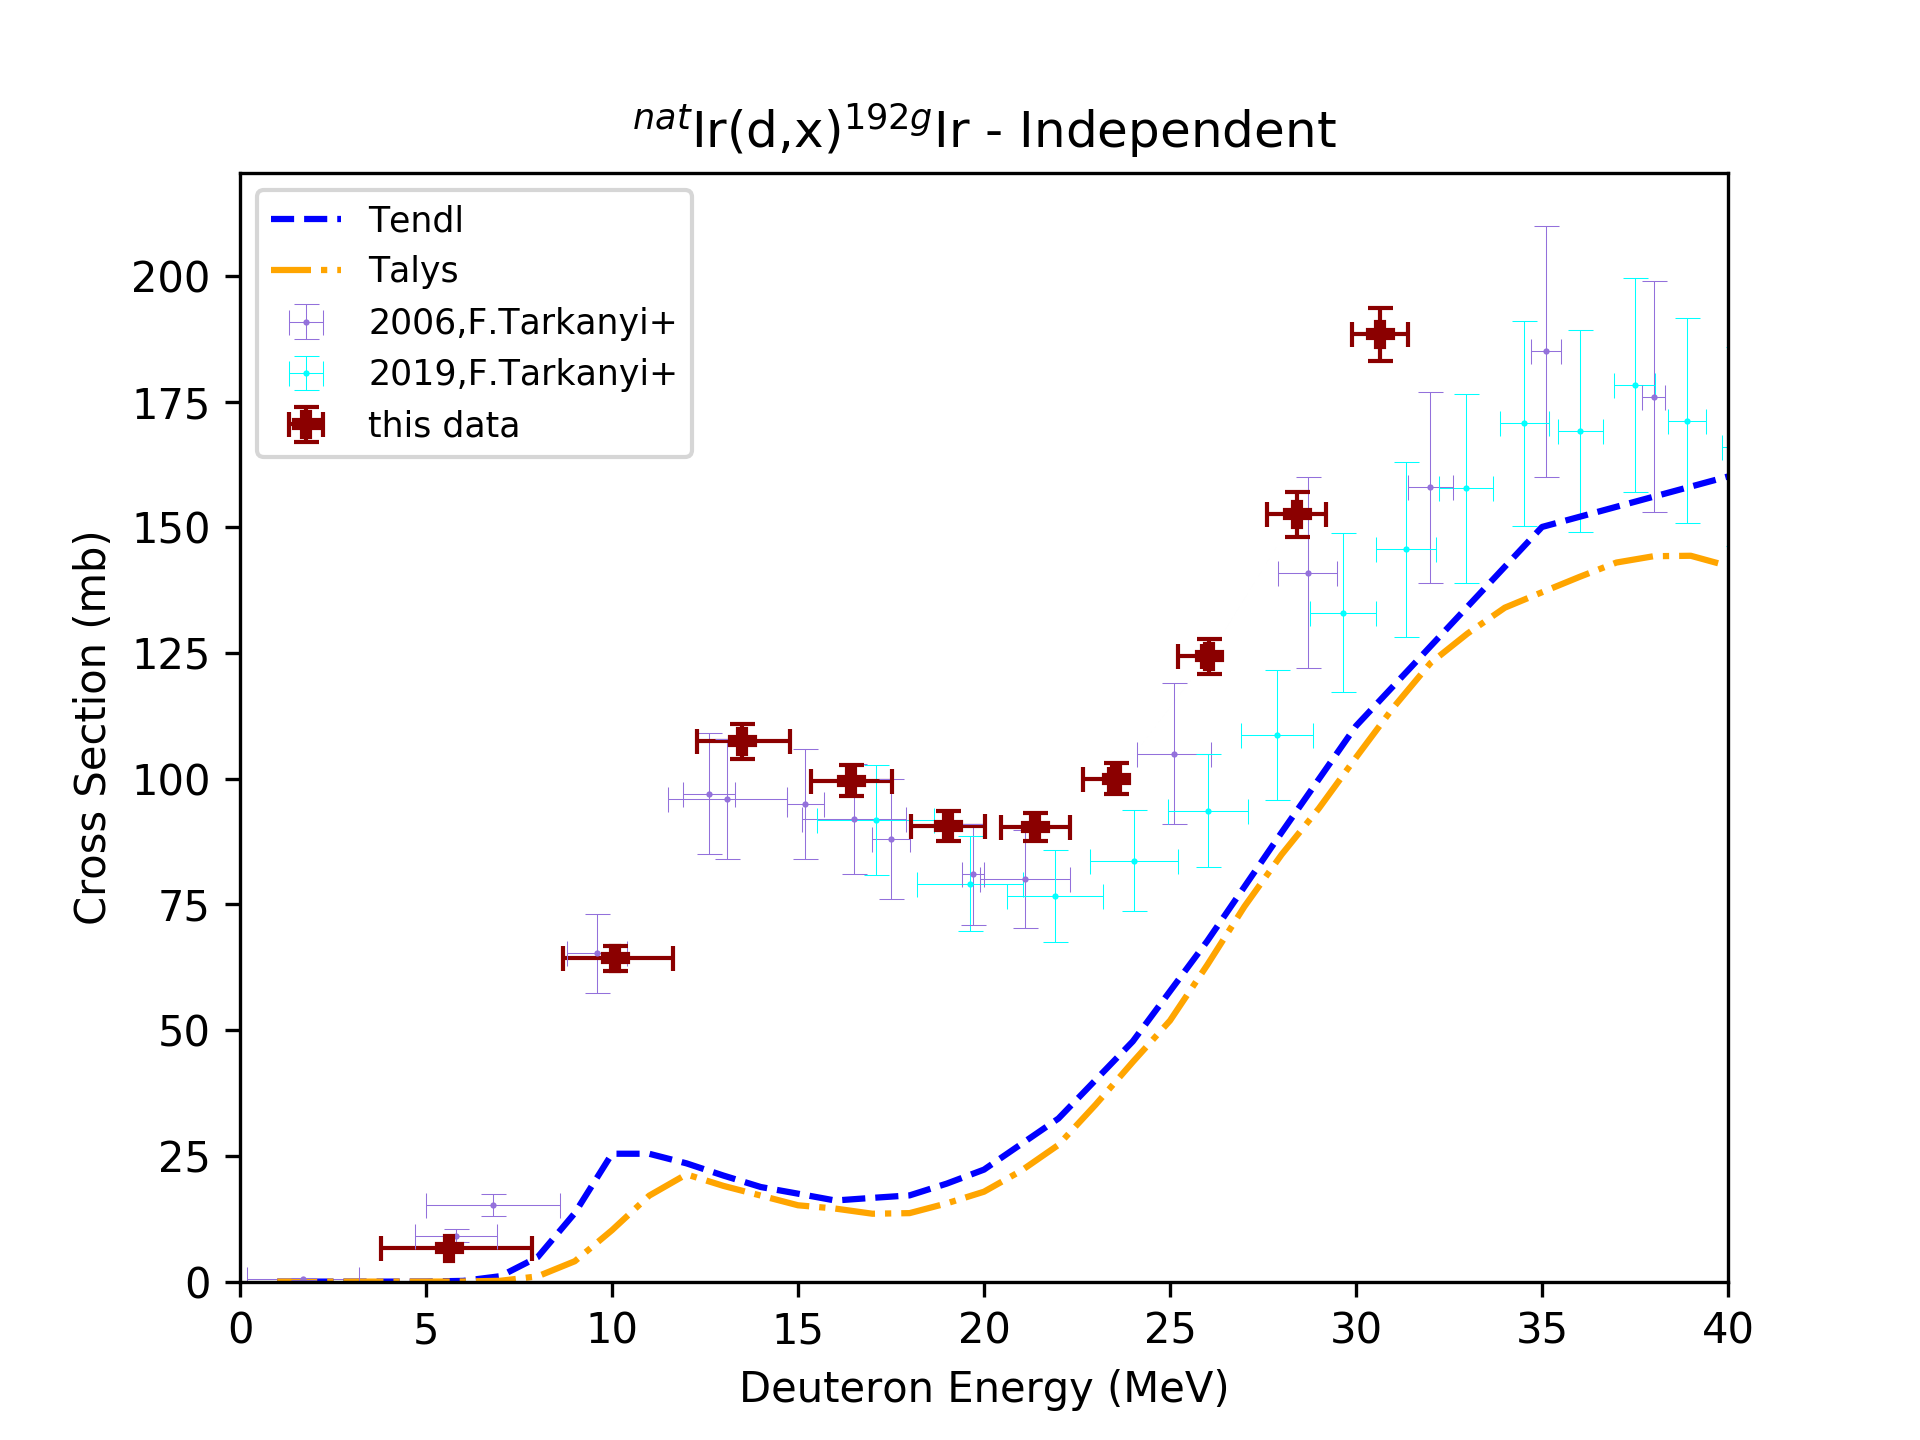
\includegraphics[width=5cm]{Results/Ir_192Ir.png} }}%
    \quad
    \subfloat[]{{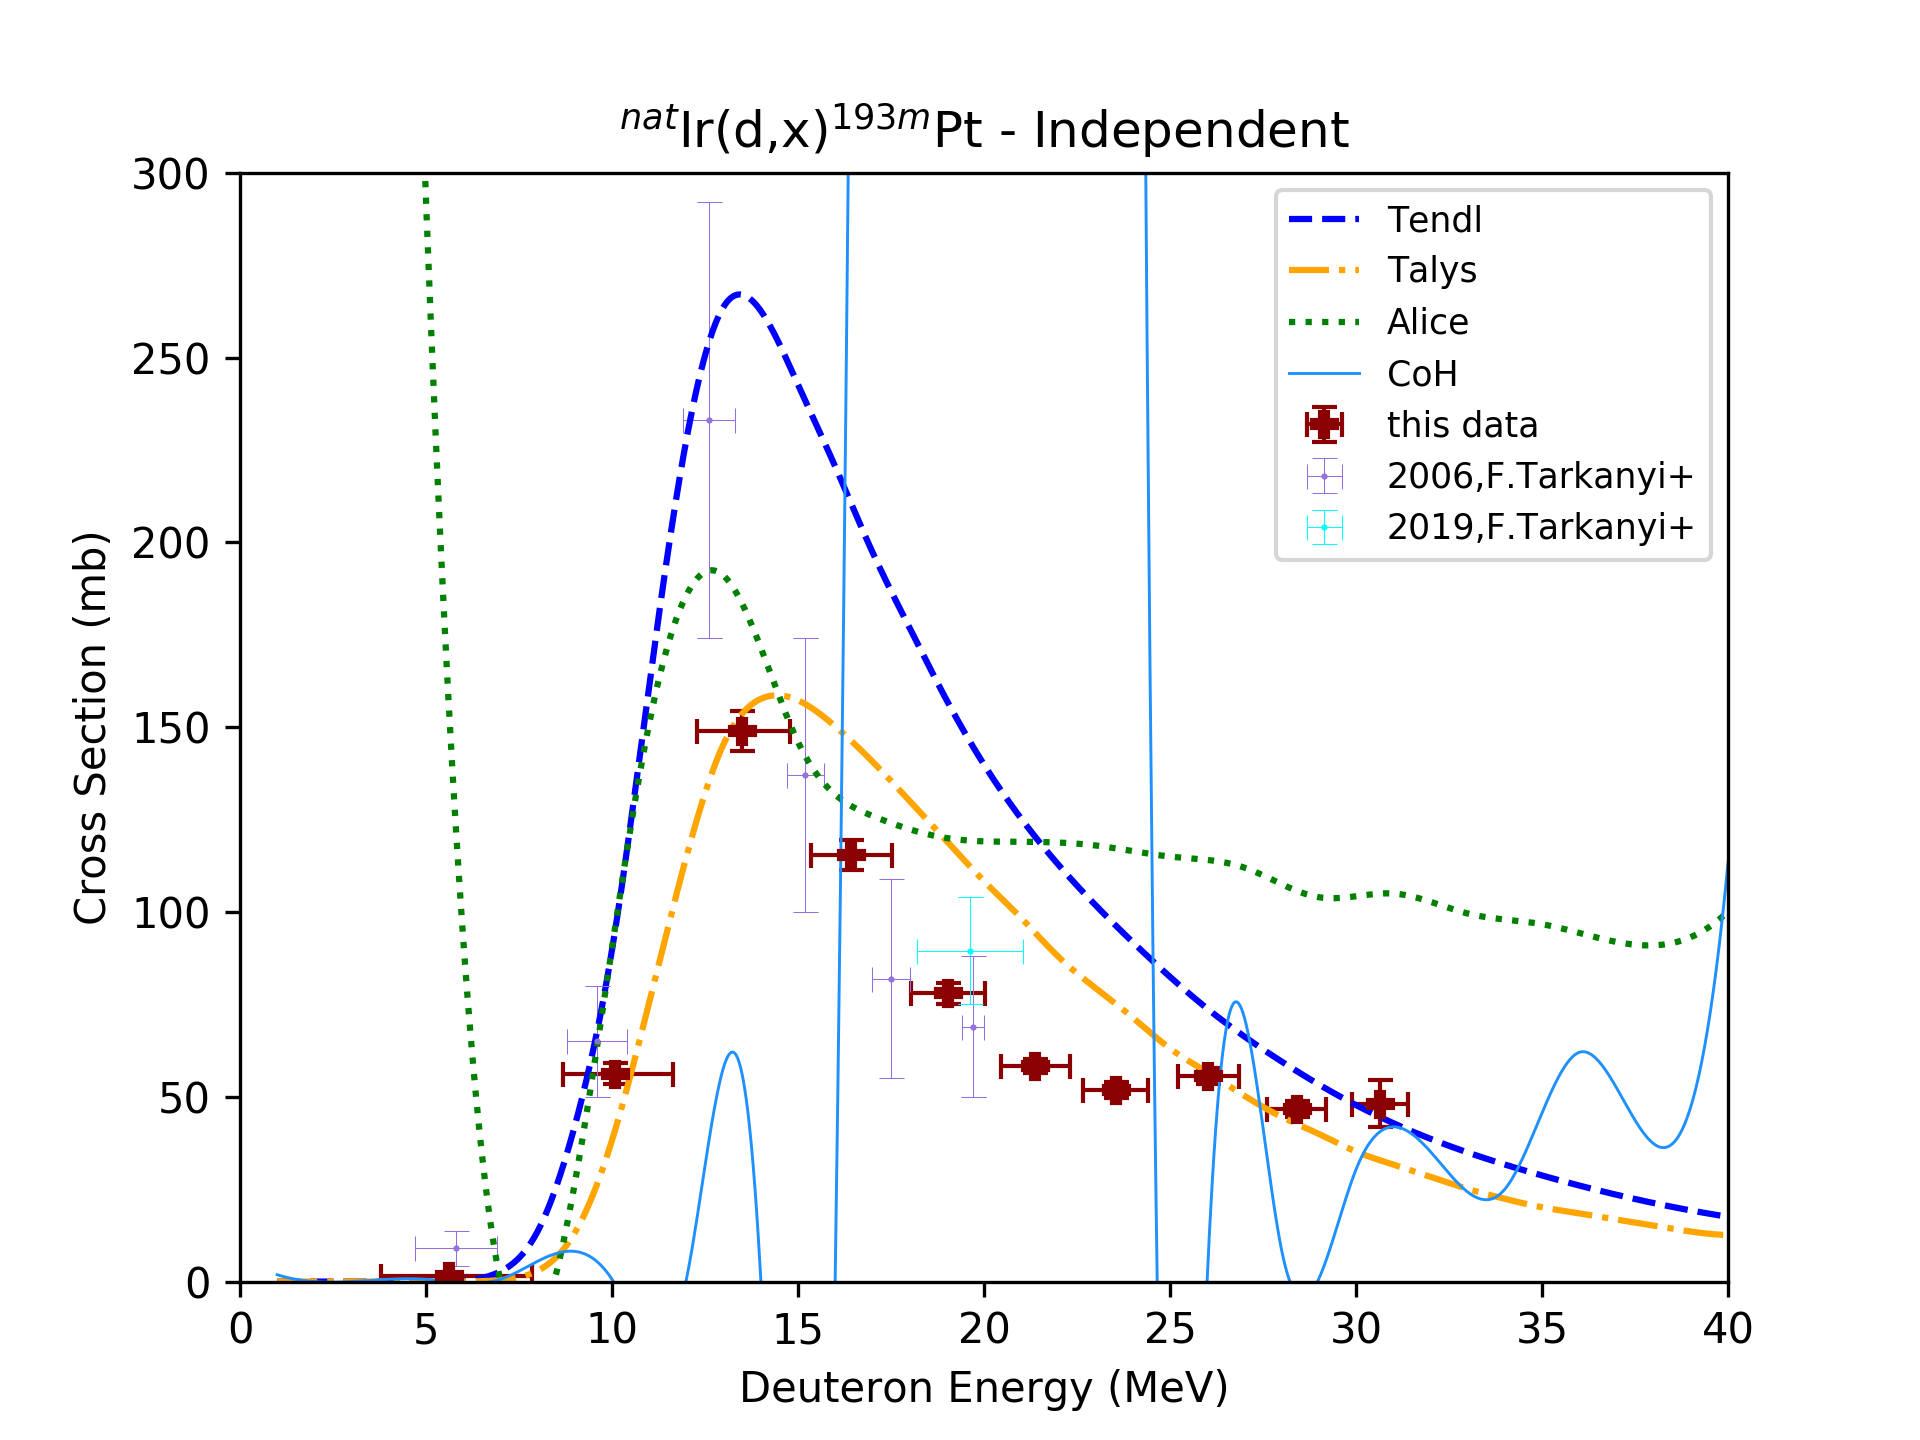
\includegraphics[width=5cm]{Results/Ir_193mPt.png} }}%
    \quad
    \subfloat[]{{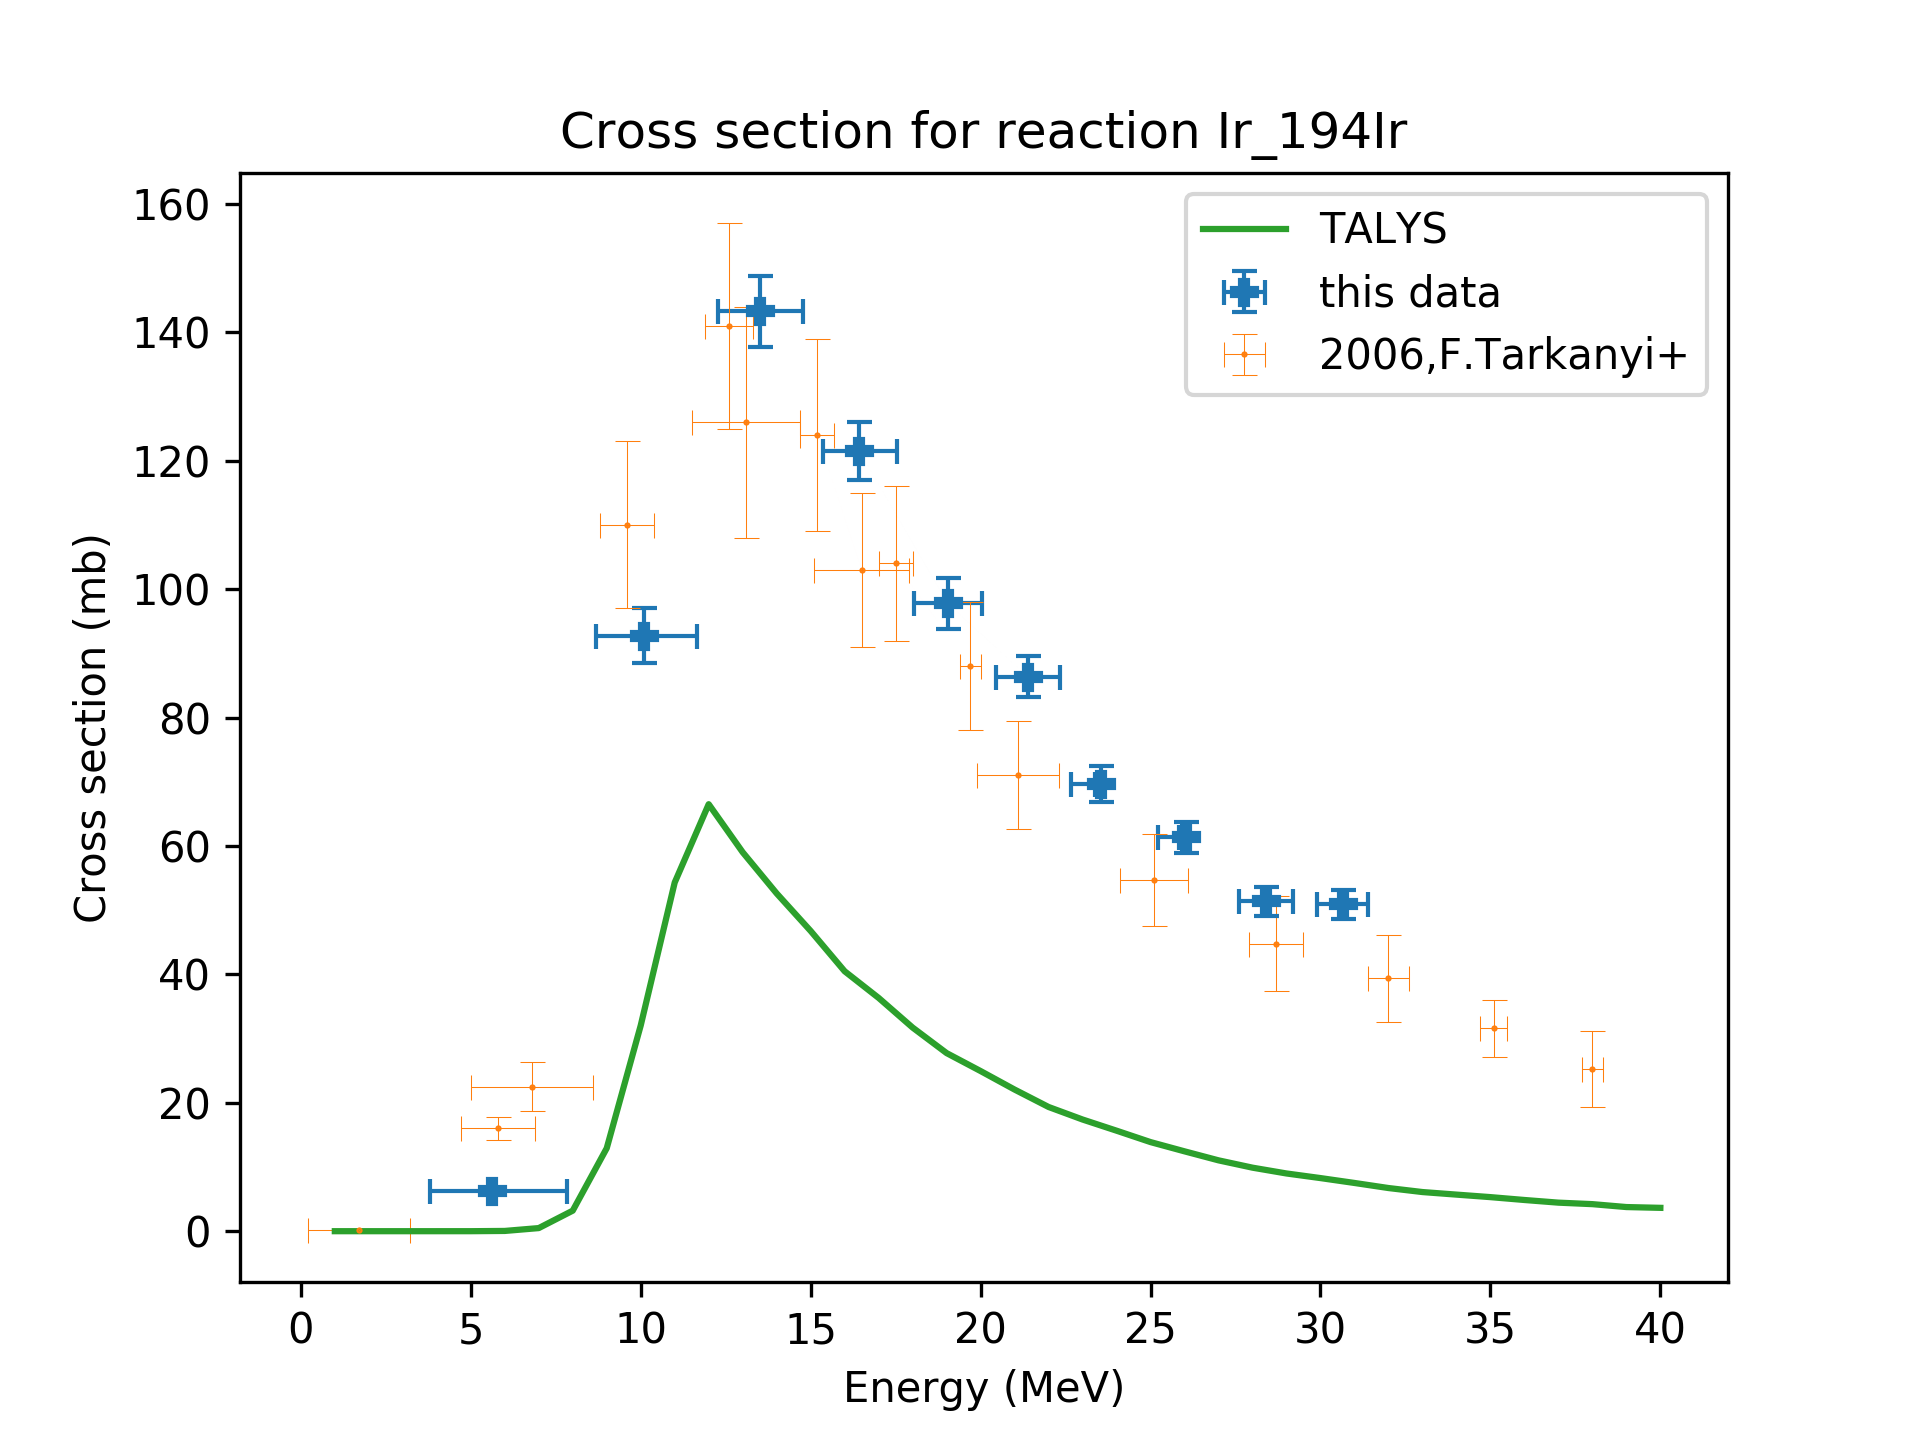
\includegraphics[width=5cm]{Results/Ir_194Ir.png} }}%
    \quad
    \subfloat[]{{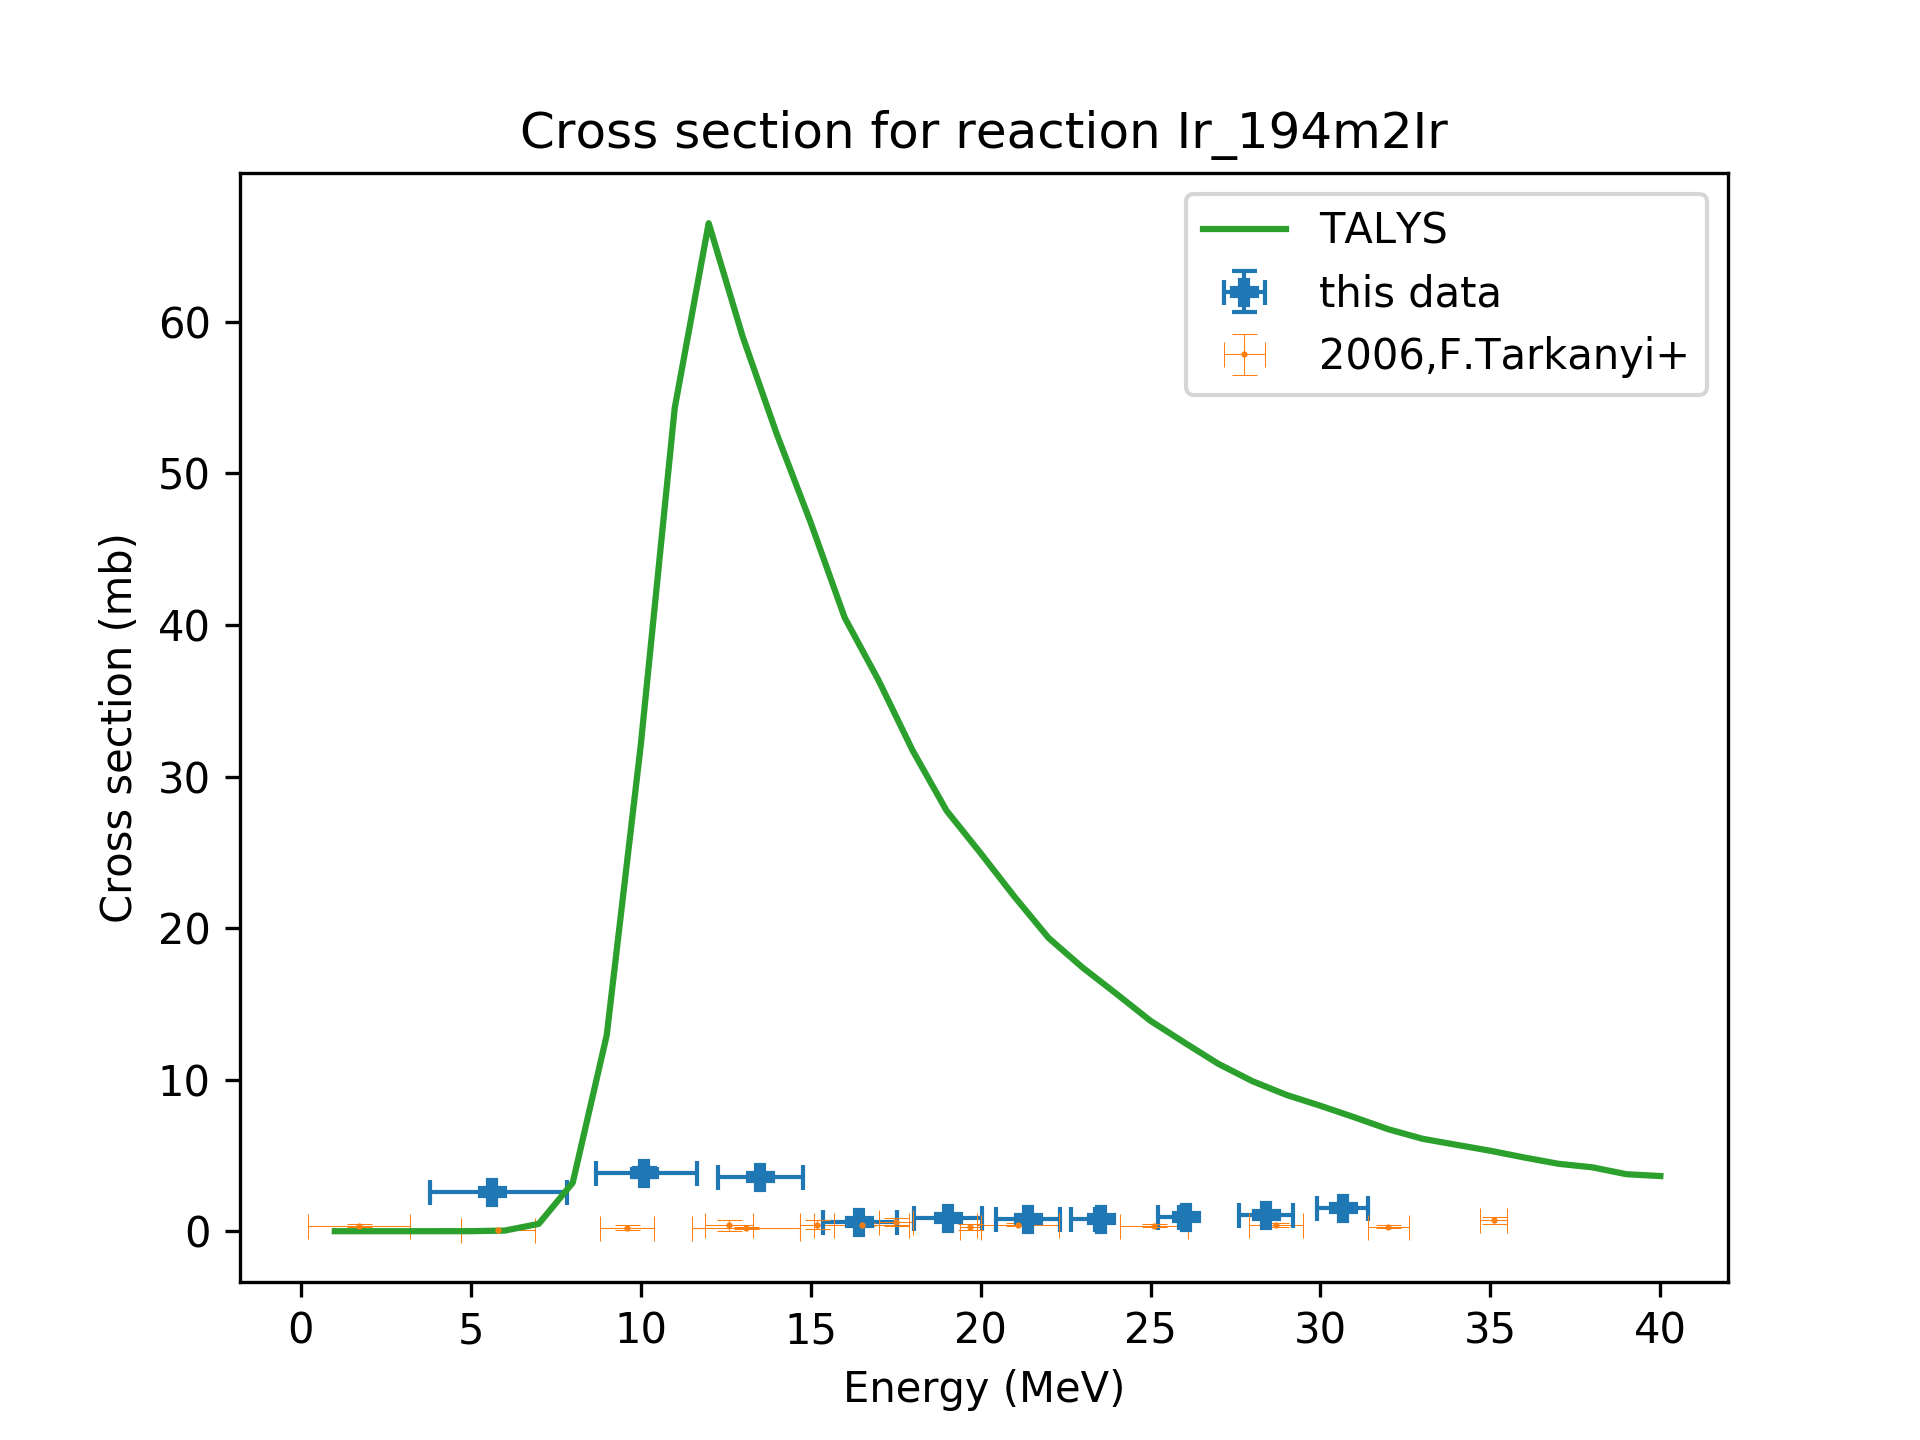
\includegraphics[width=5cm]{Results/Ir_194m2Ir.png} }}%
    \quad
    \caption{Iridium cross sections }%
    \label{fig:Ir_crosssections}%
\end{figure}

\section{Nickel cross sections}

\begin{figure}%
    \centering
    \subfloat[]{{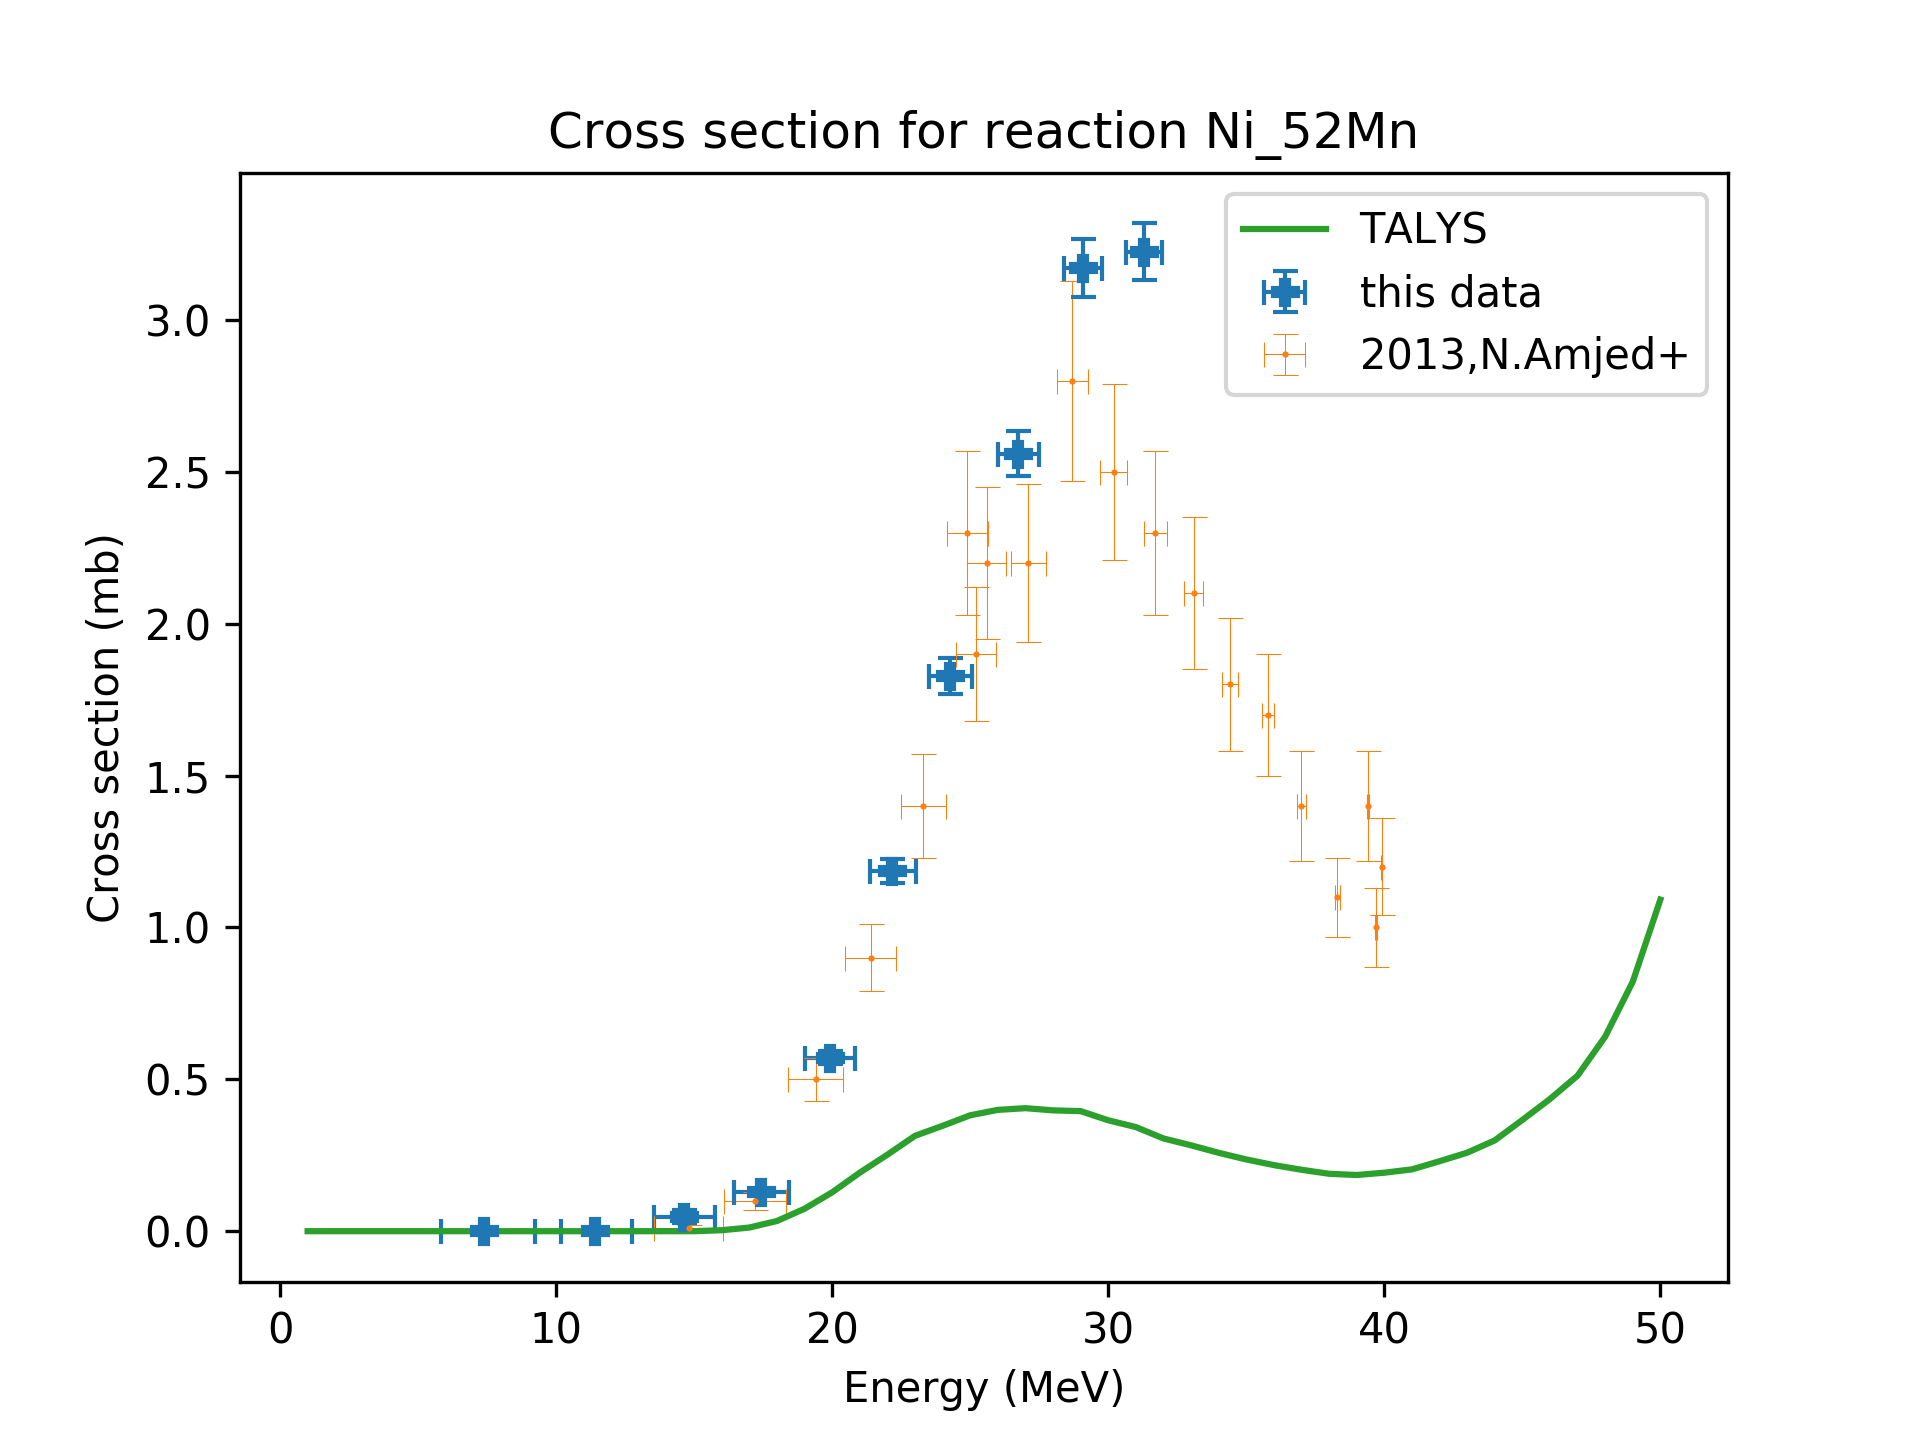
\includegraphics[width=5cm]{Results/Ni_52Mn.png}}%
    \quad
    \subfloat[]{{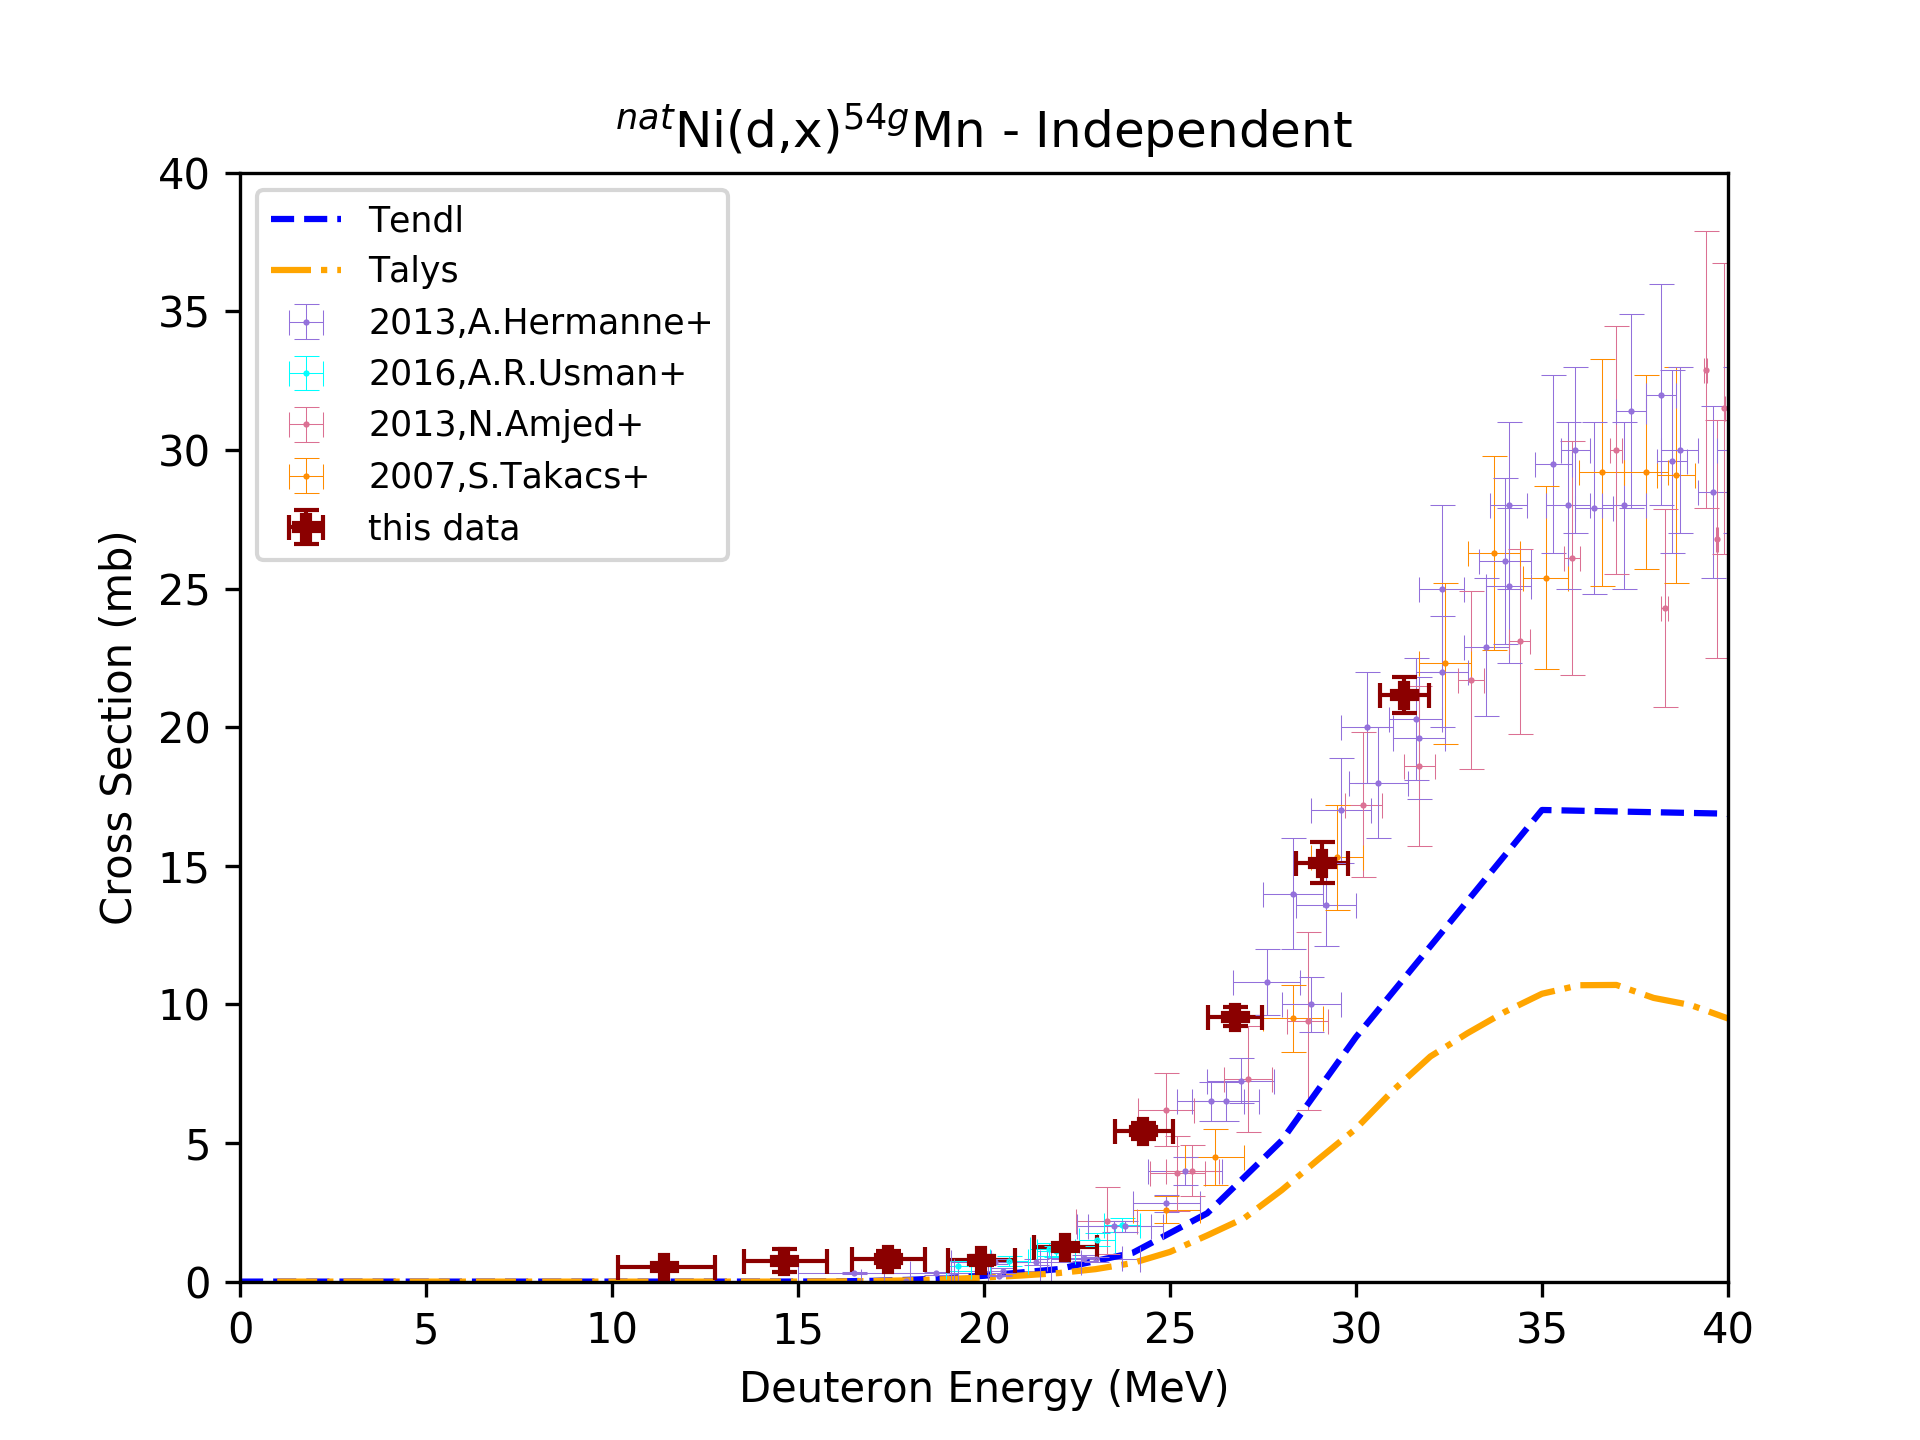
\includegraphics[width=5cm]{Results/Ni_54Mn.png} }}%
    \subfloat[]{{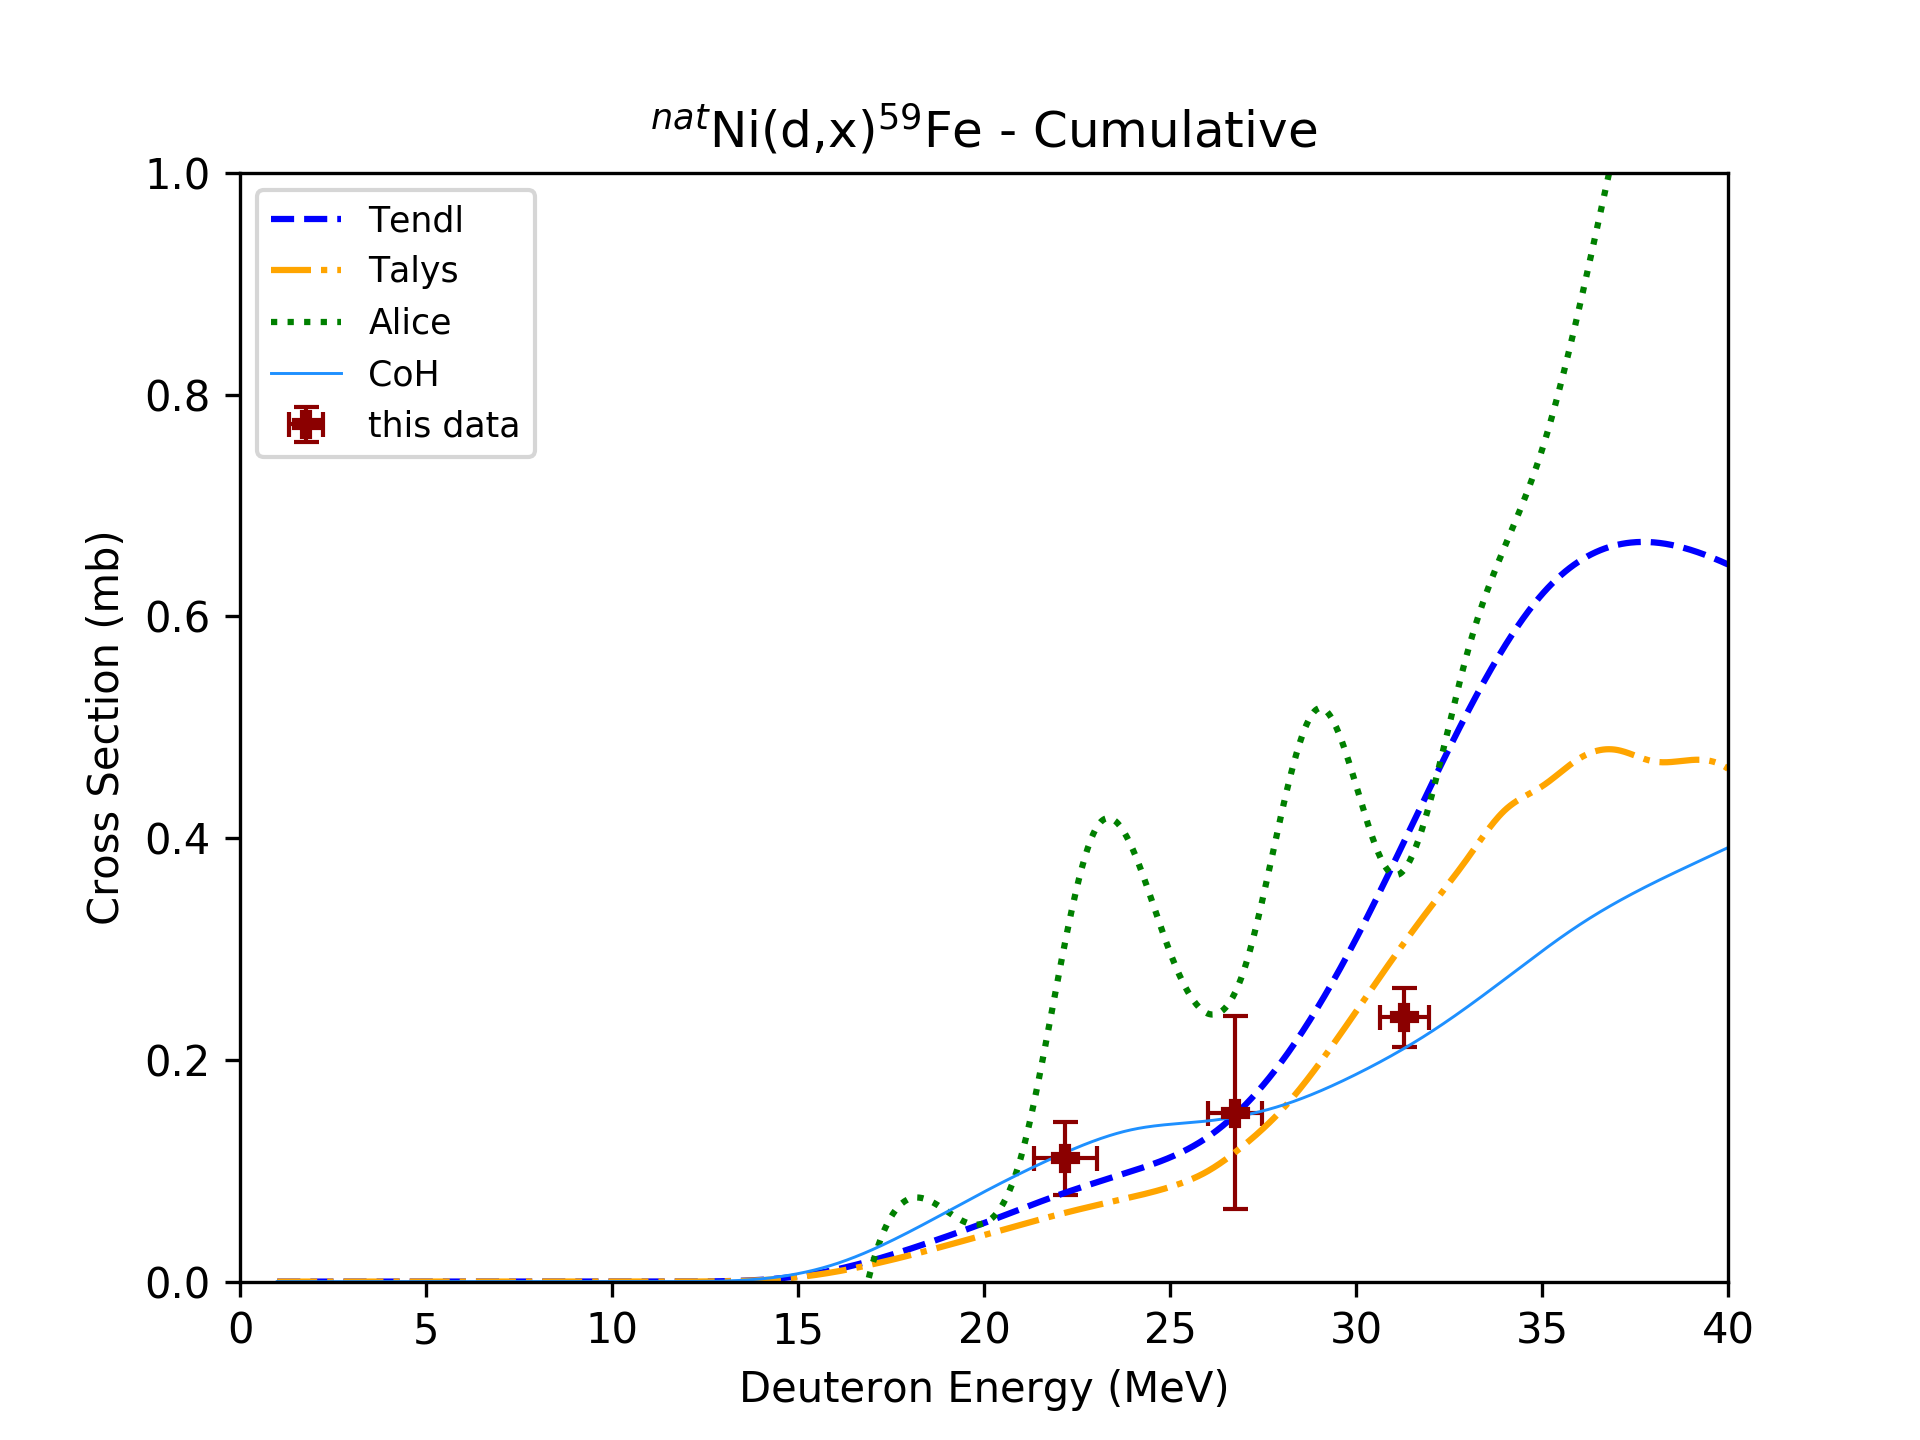
\includegraphics[width=5cm]{Results/Ni_59Fe.png} }}%
    \quad
    \subfloat[]{{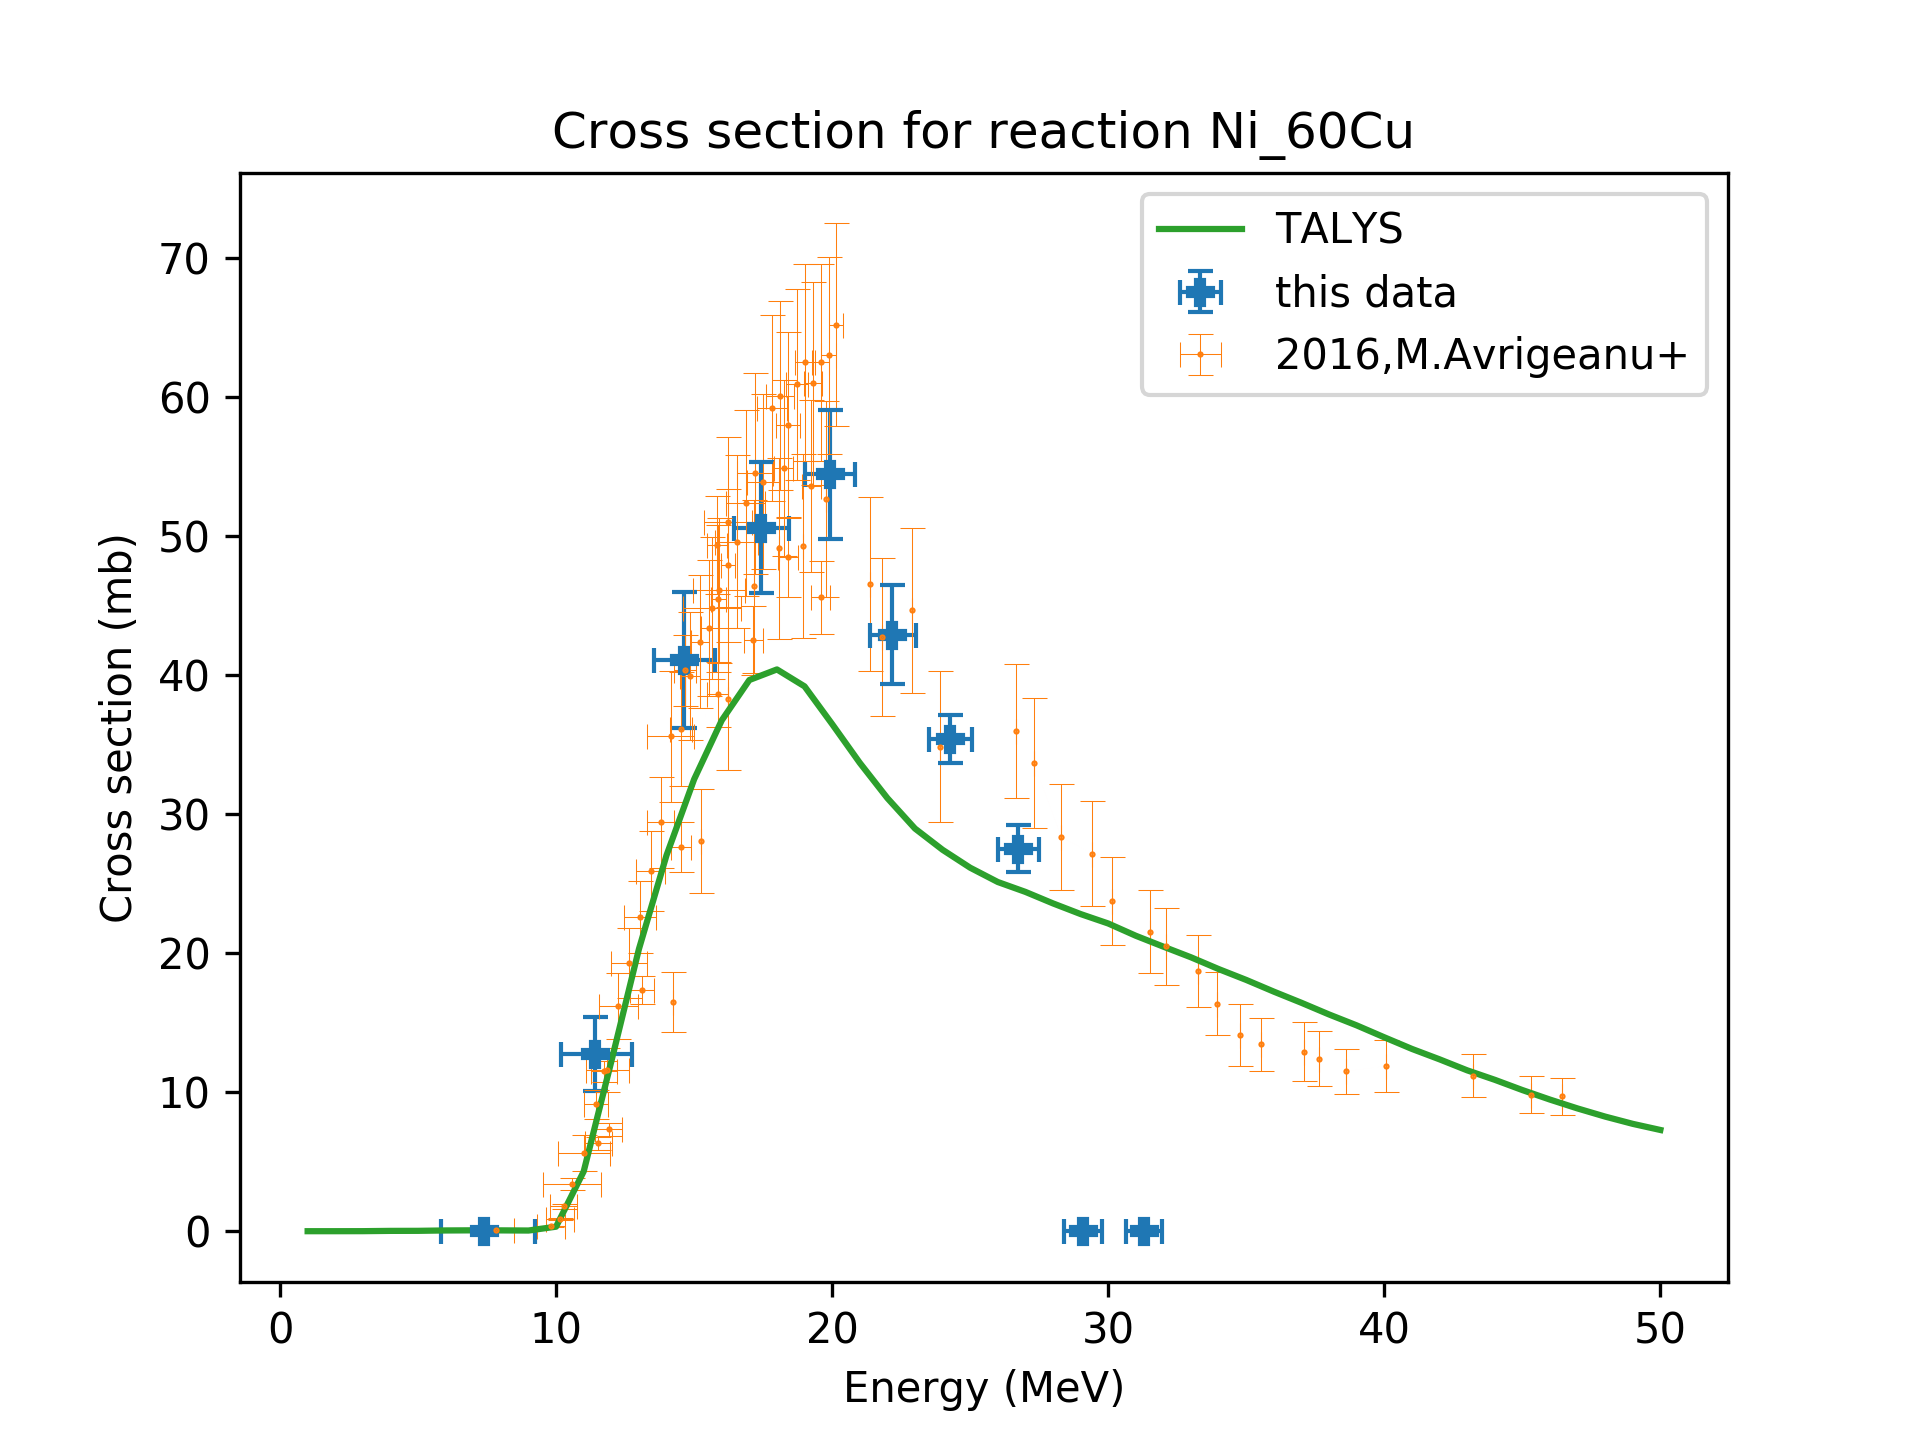
\includegraphics[width=5cm]{Results/Ni_60Cu.png} }}%
    \quad
    \subfloat[]{{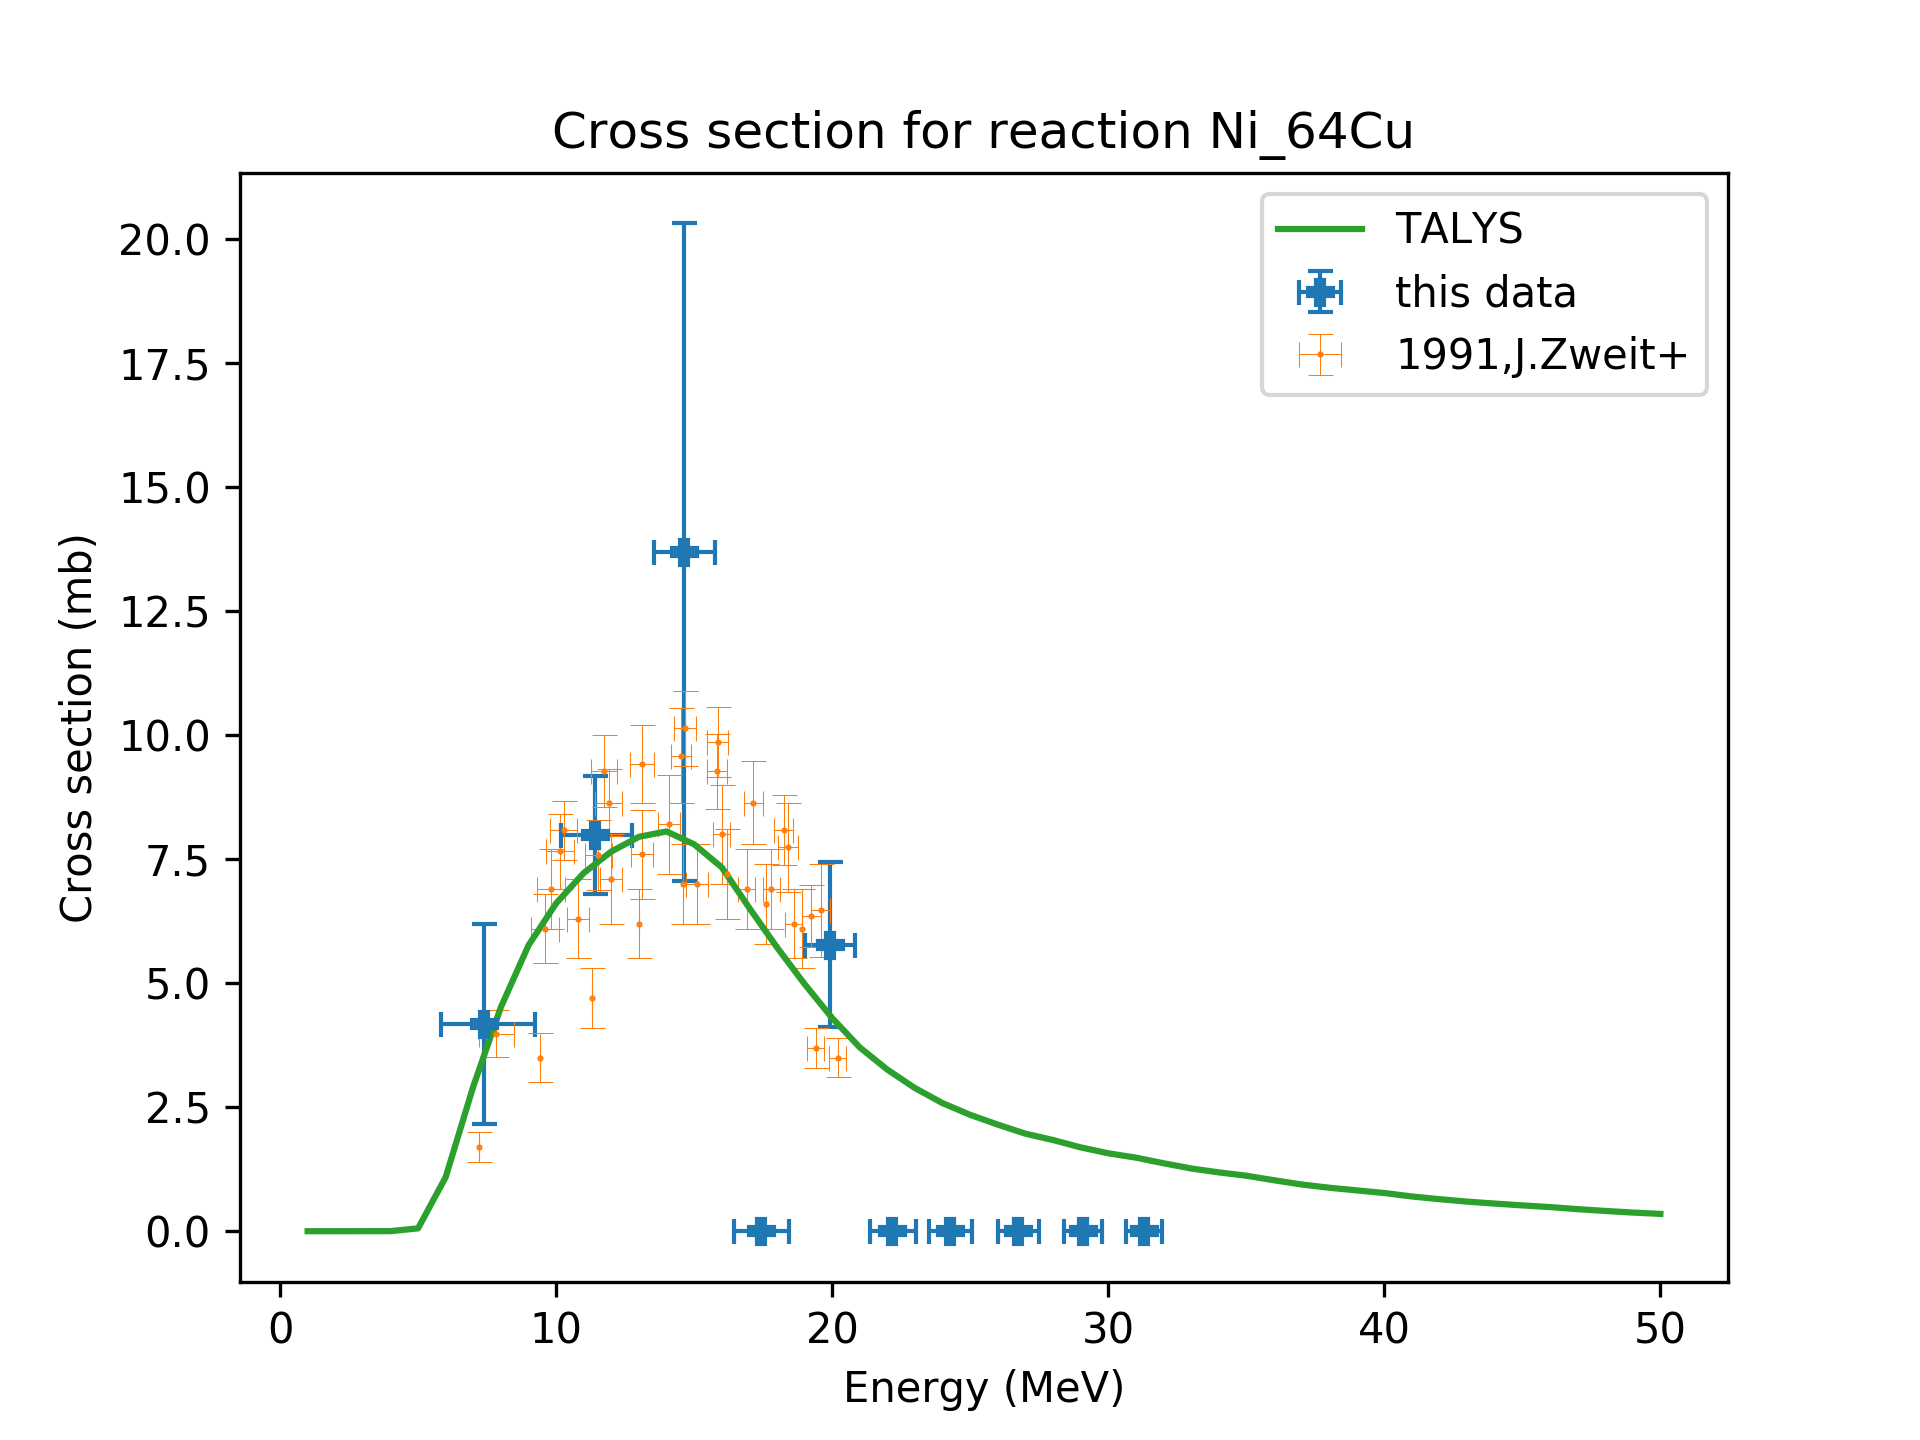
\includegraphics[width=5cm]{Results/Ni_64Cu.png} }}%
    \quad
    \subfloat[caption]{{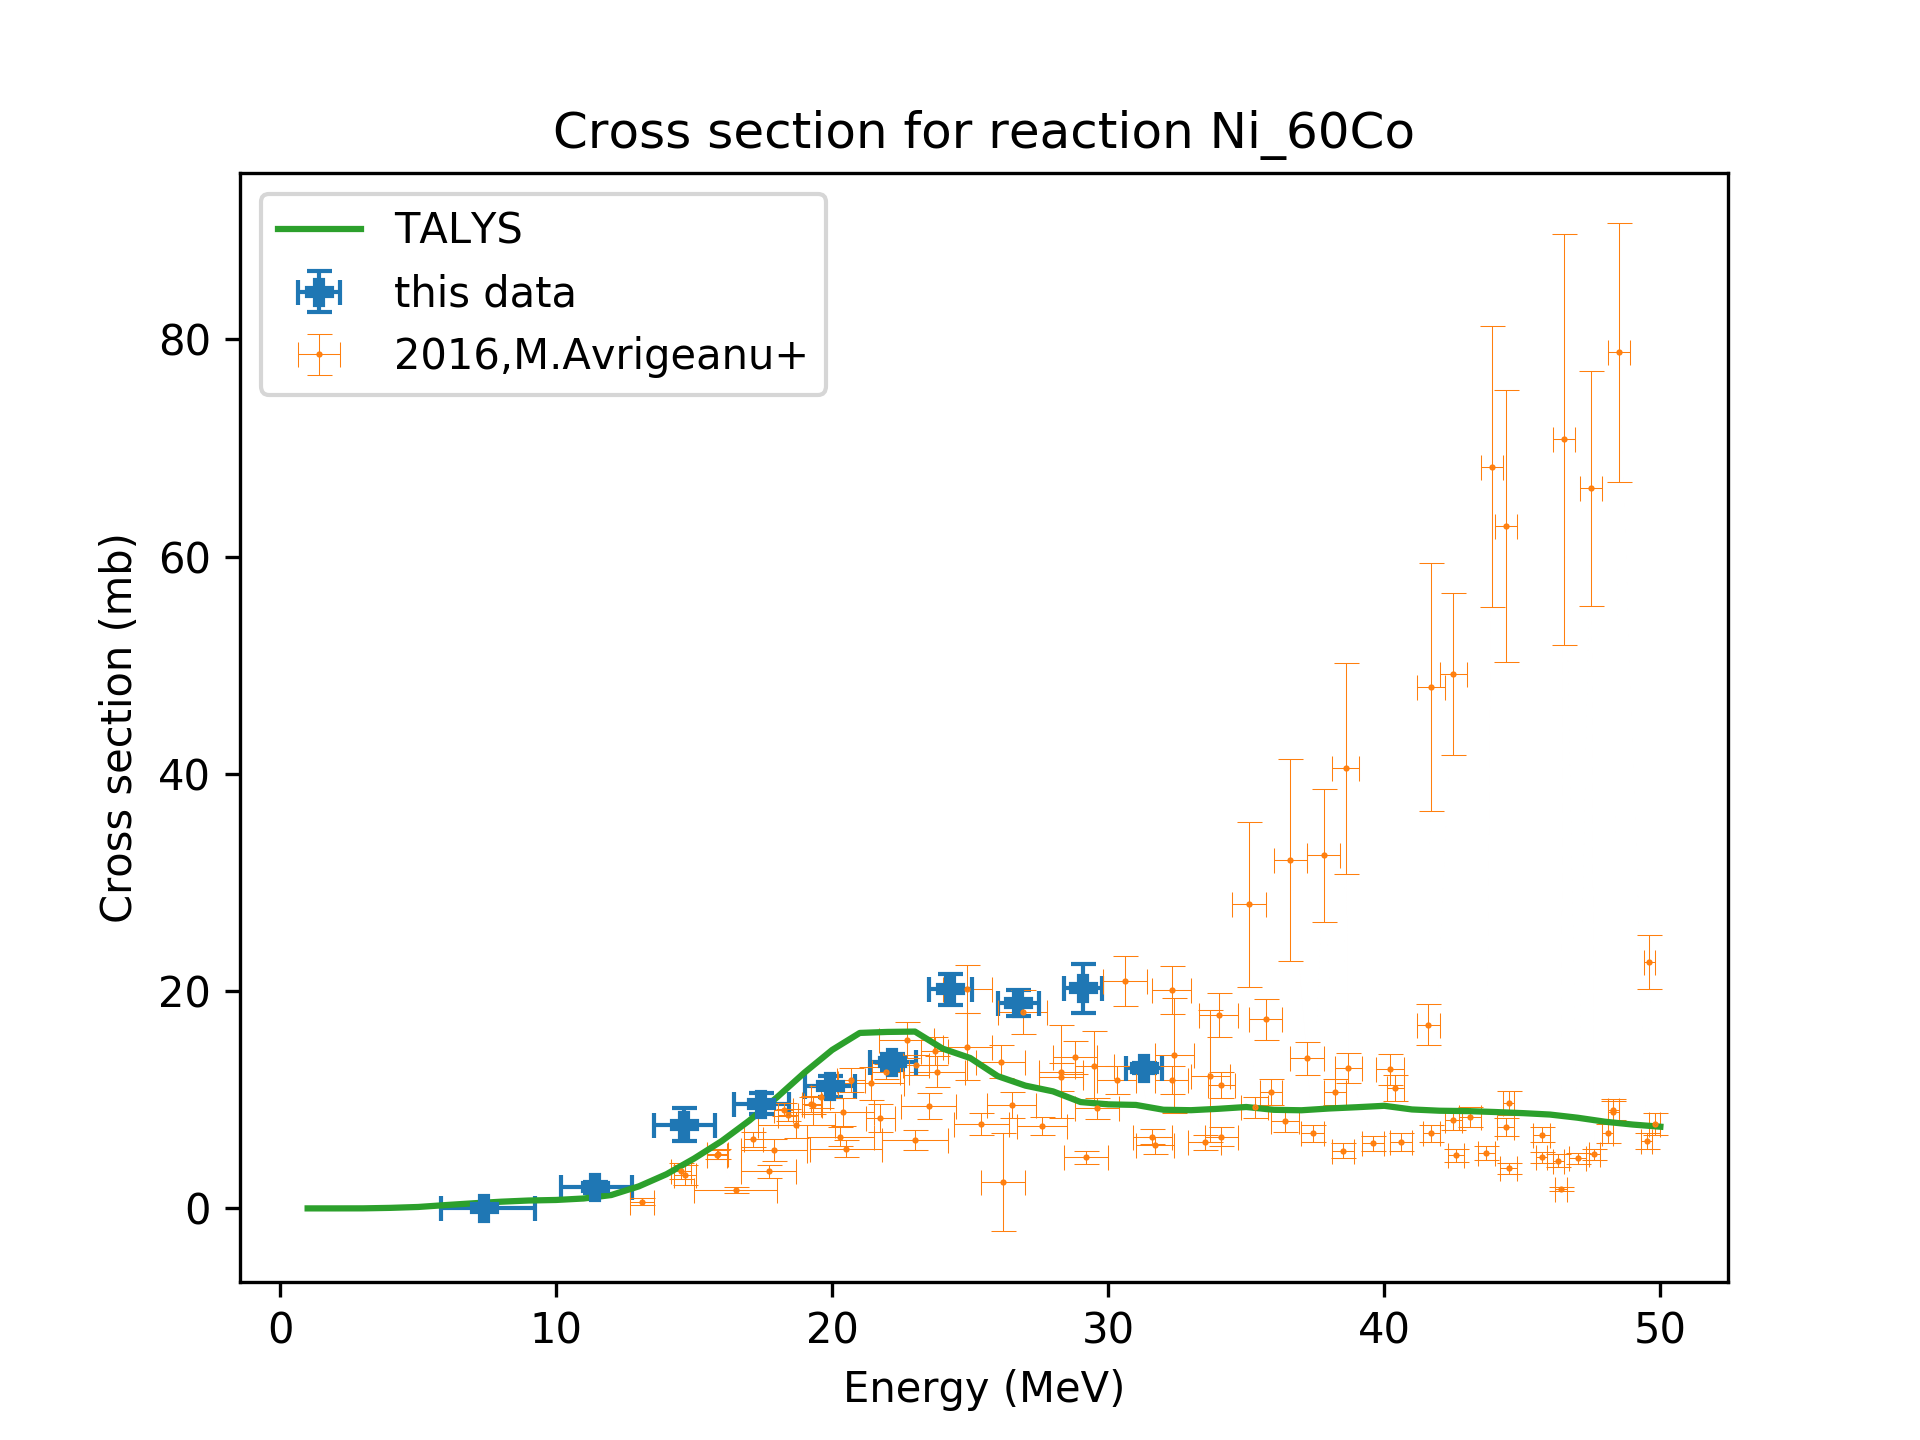
\includegraphics[width=5cm]{Results/Ni_60Co.png} }}%
    \quad
    \subfloat[]{{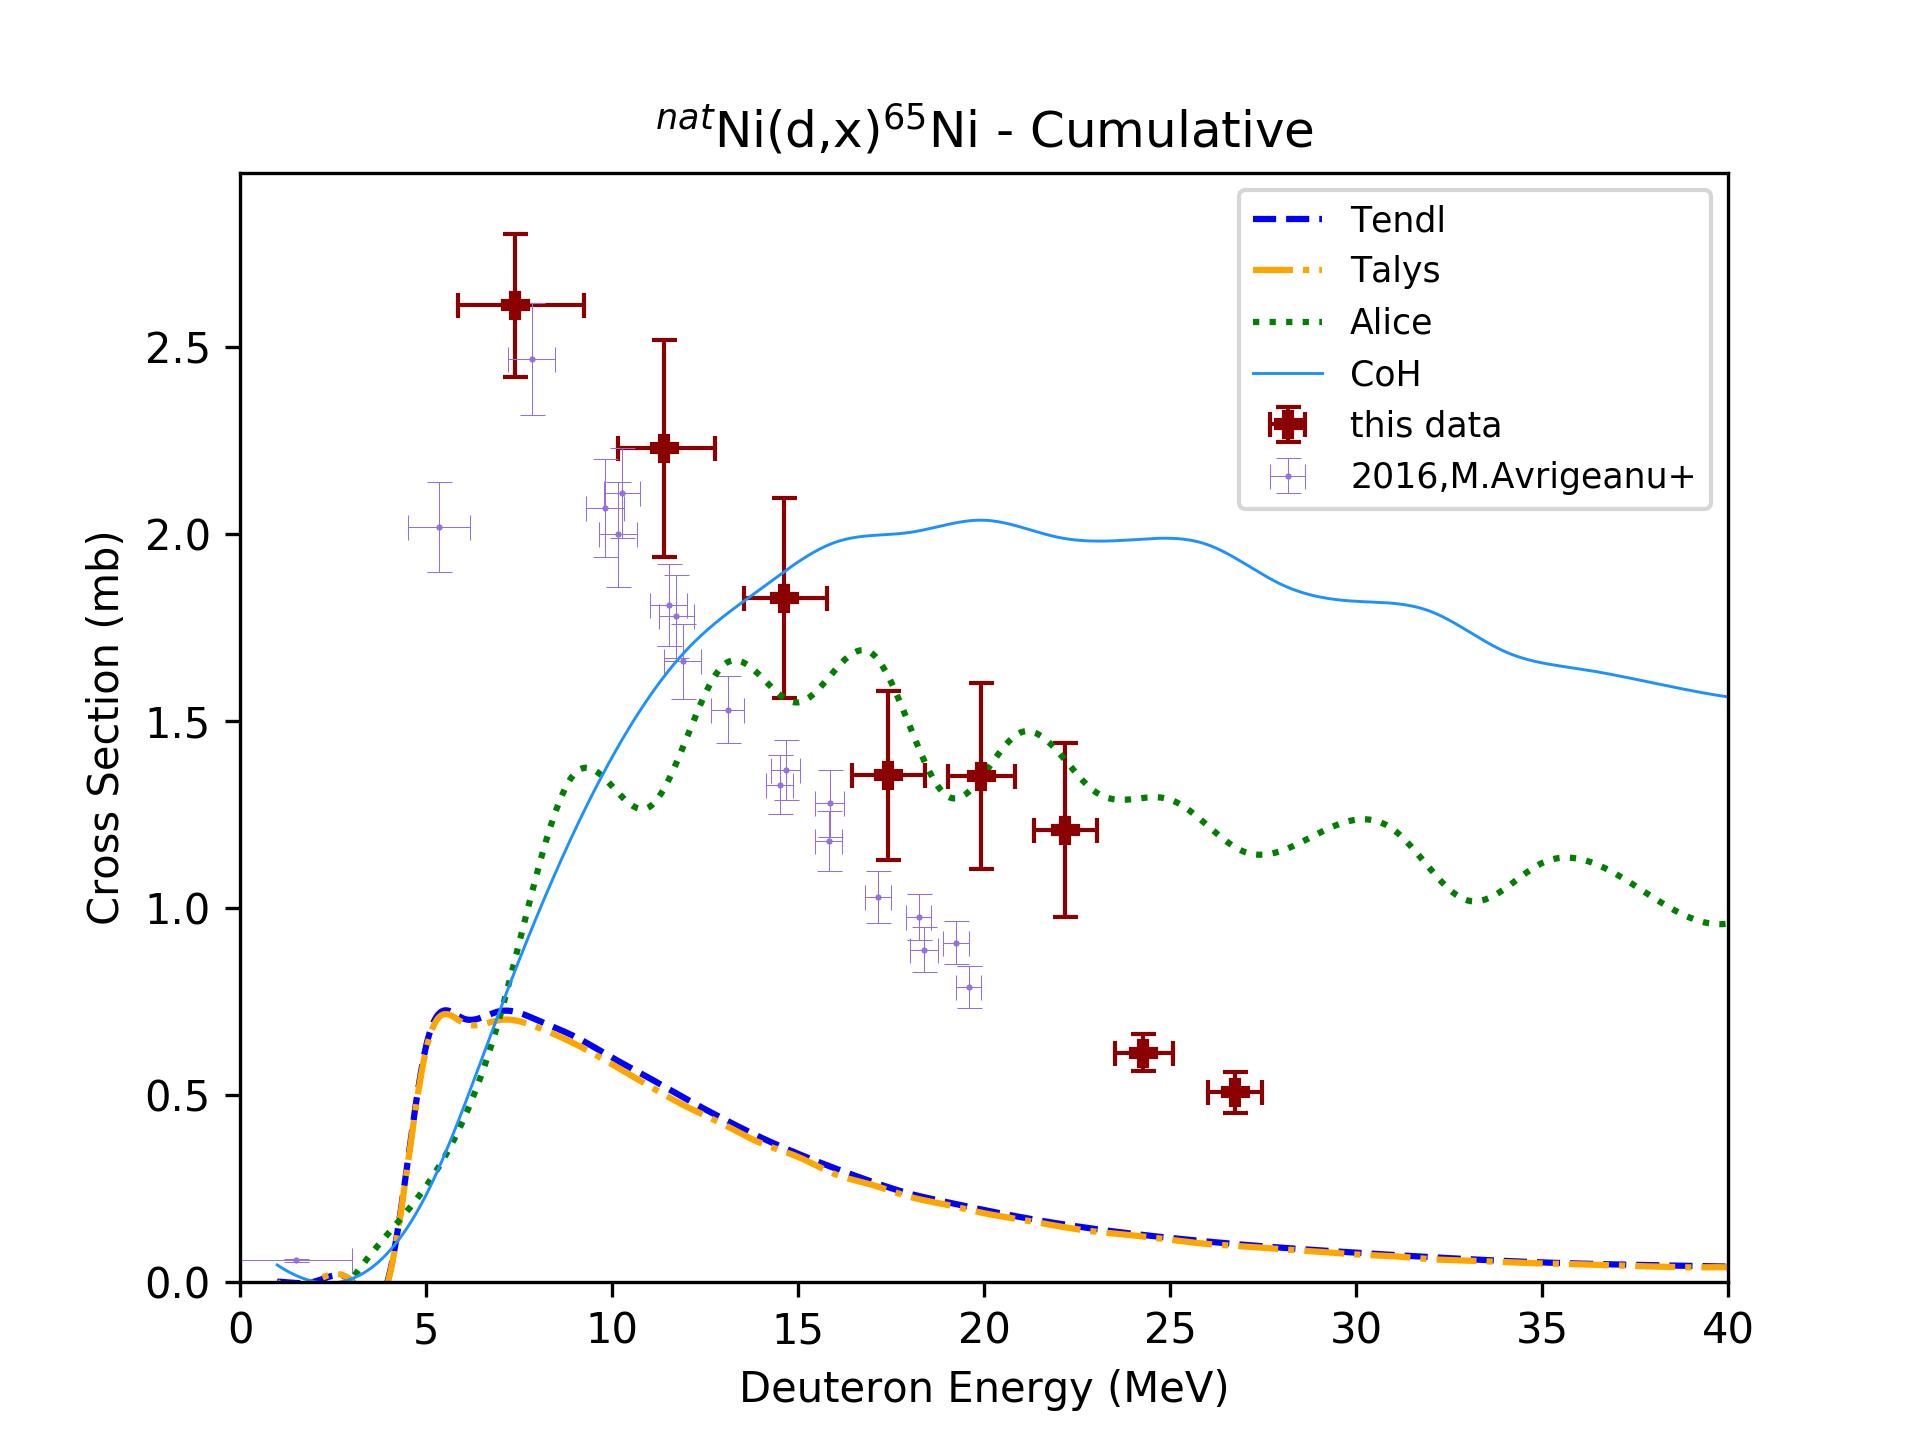
\includegraphics[width=5cm]{Results/Ni_65Ni.png} }}%
    \quad
    \subfloat[]{{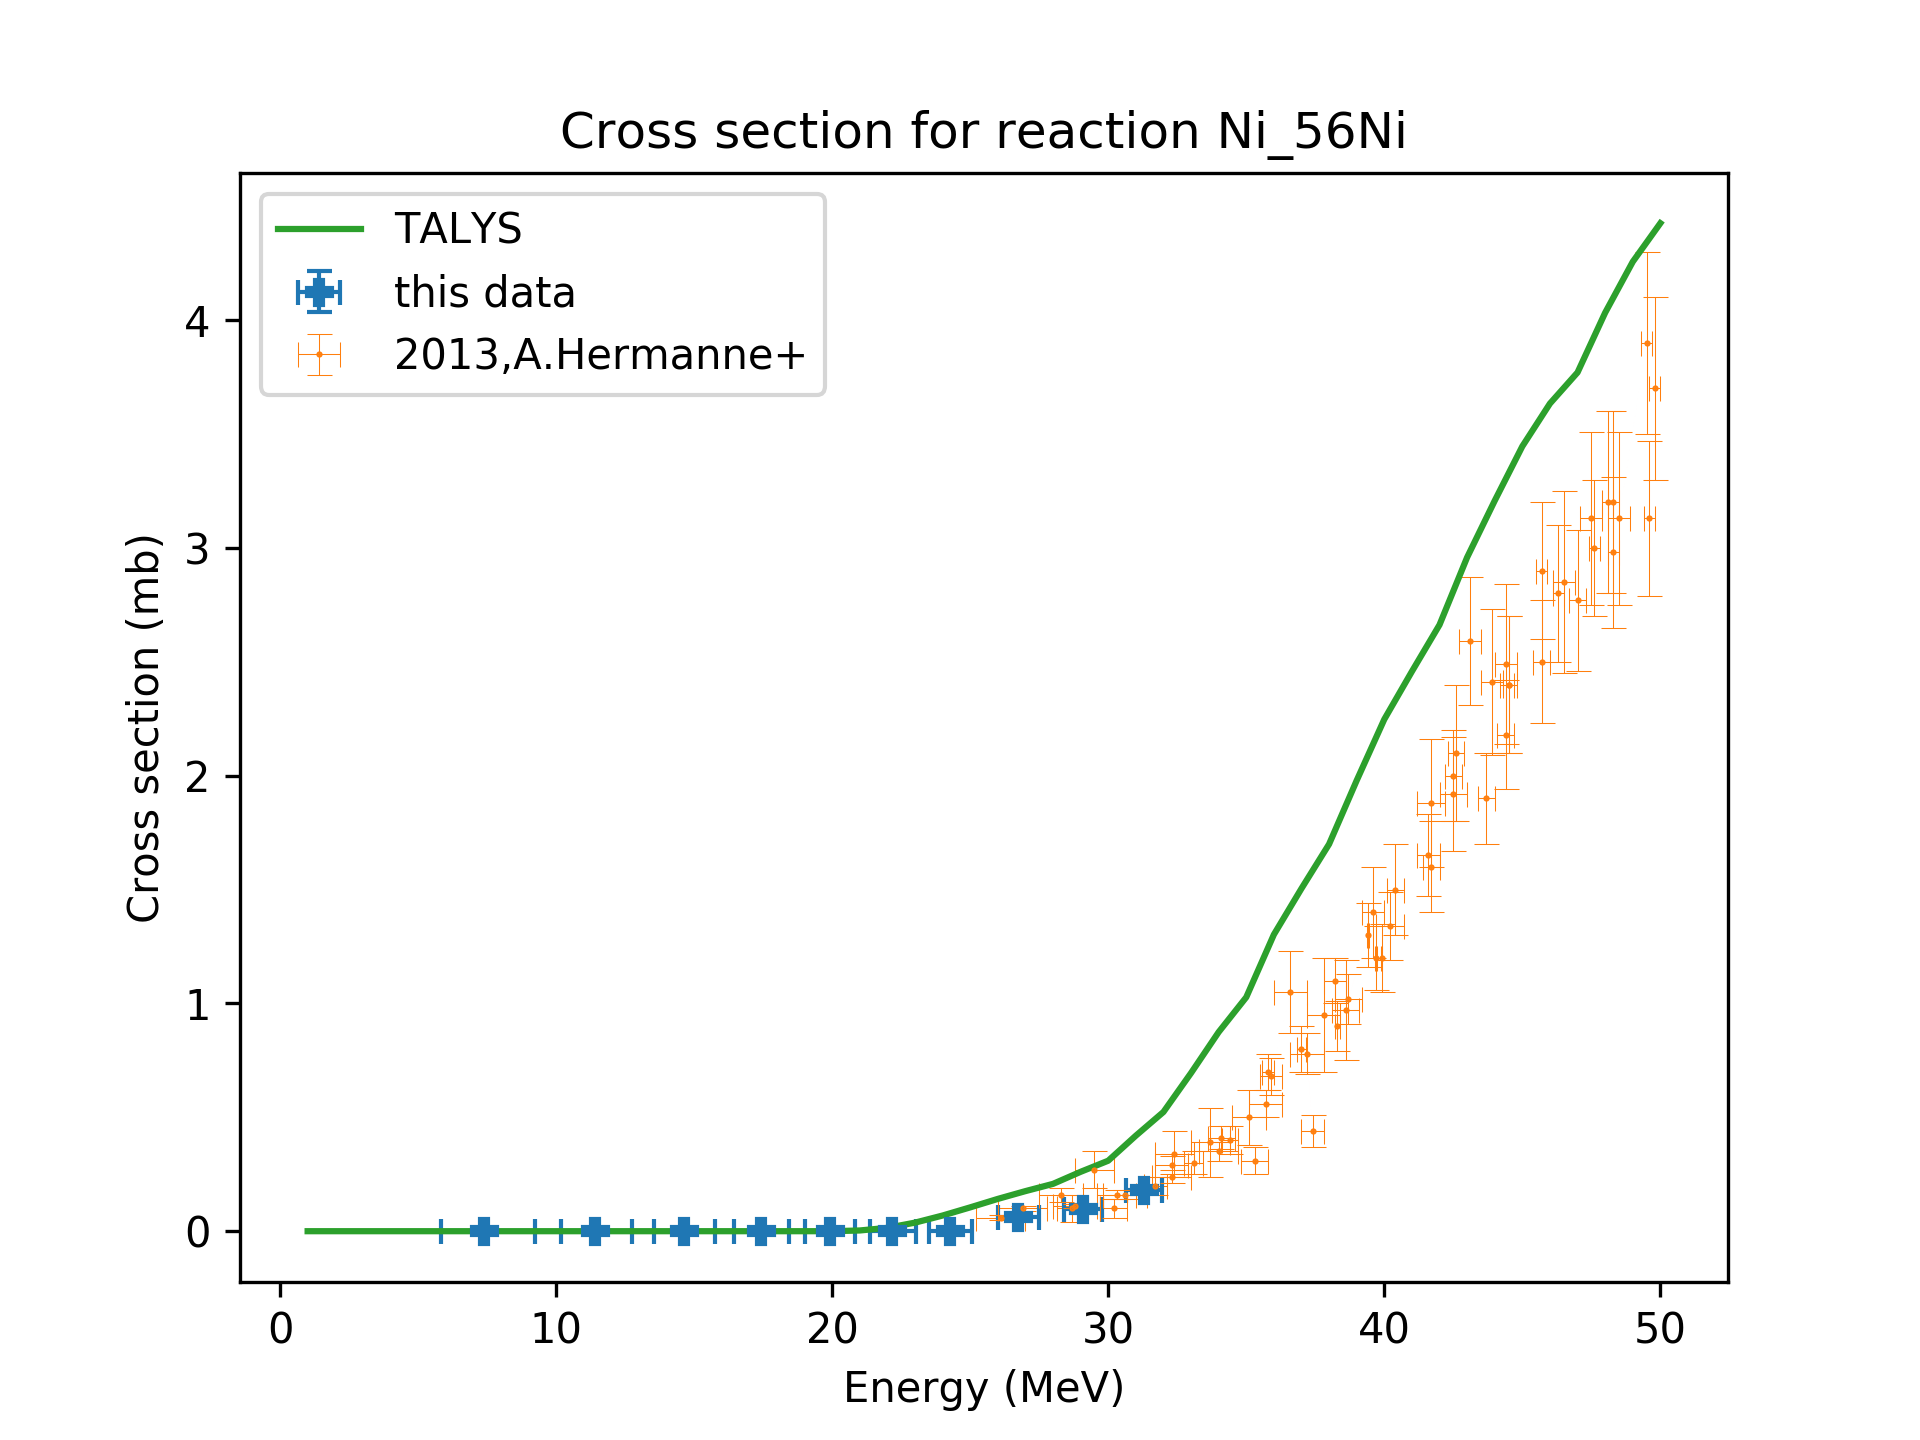
\includegraphics[width=5cm]{Results/Ni_56Ni.png} }}%
    \quad
    \subfloat[]{{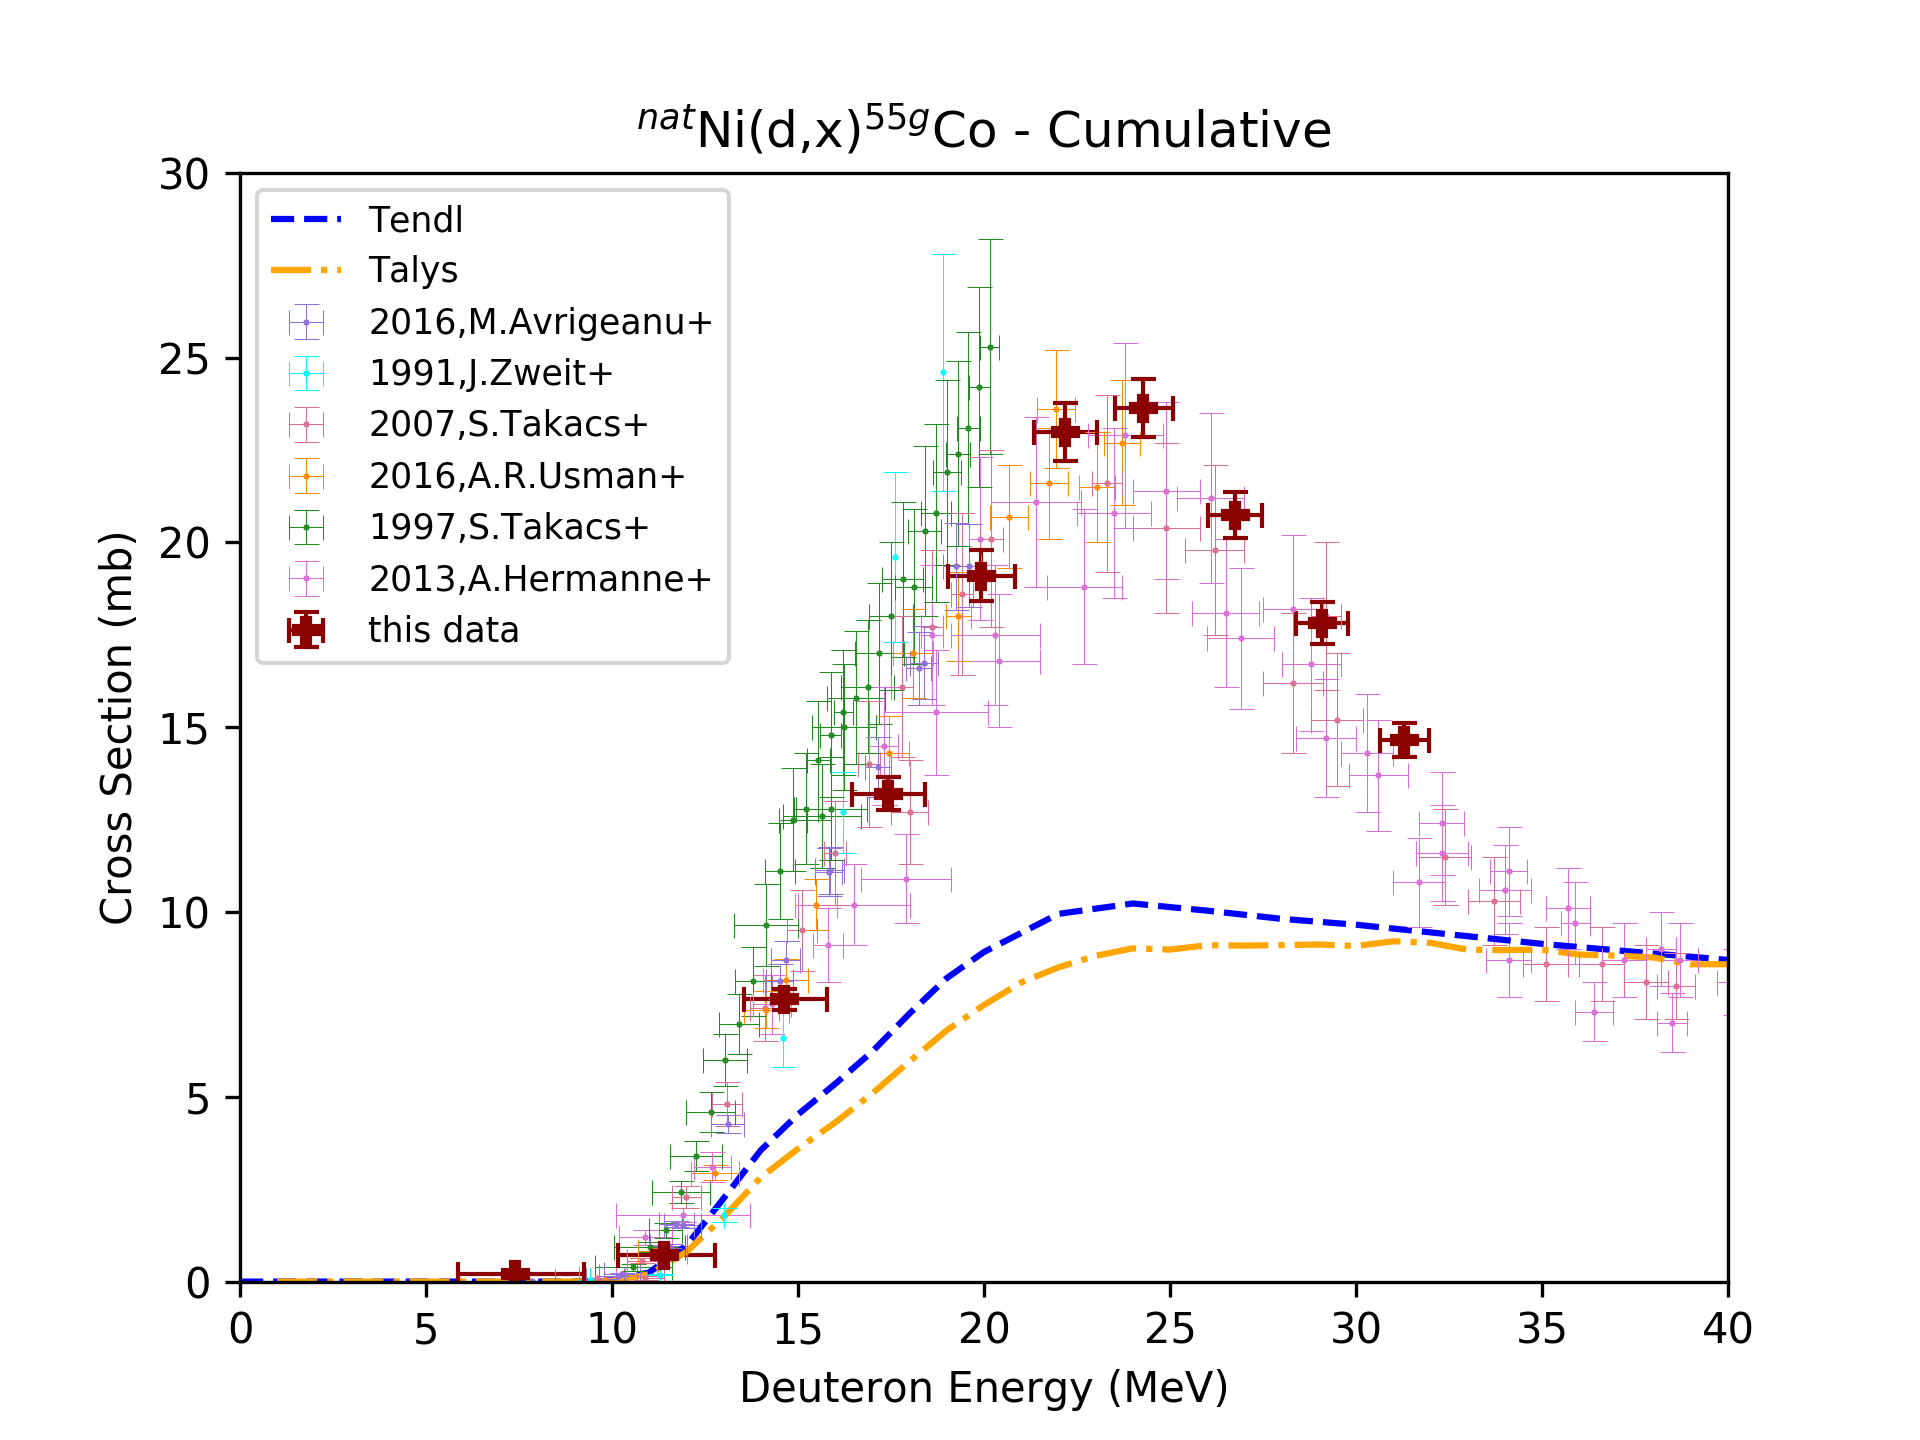
\includegraphics[width=5cm]{Results/Ni_55Co.png} }}%
    \quad
    \subfloat[]{{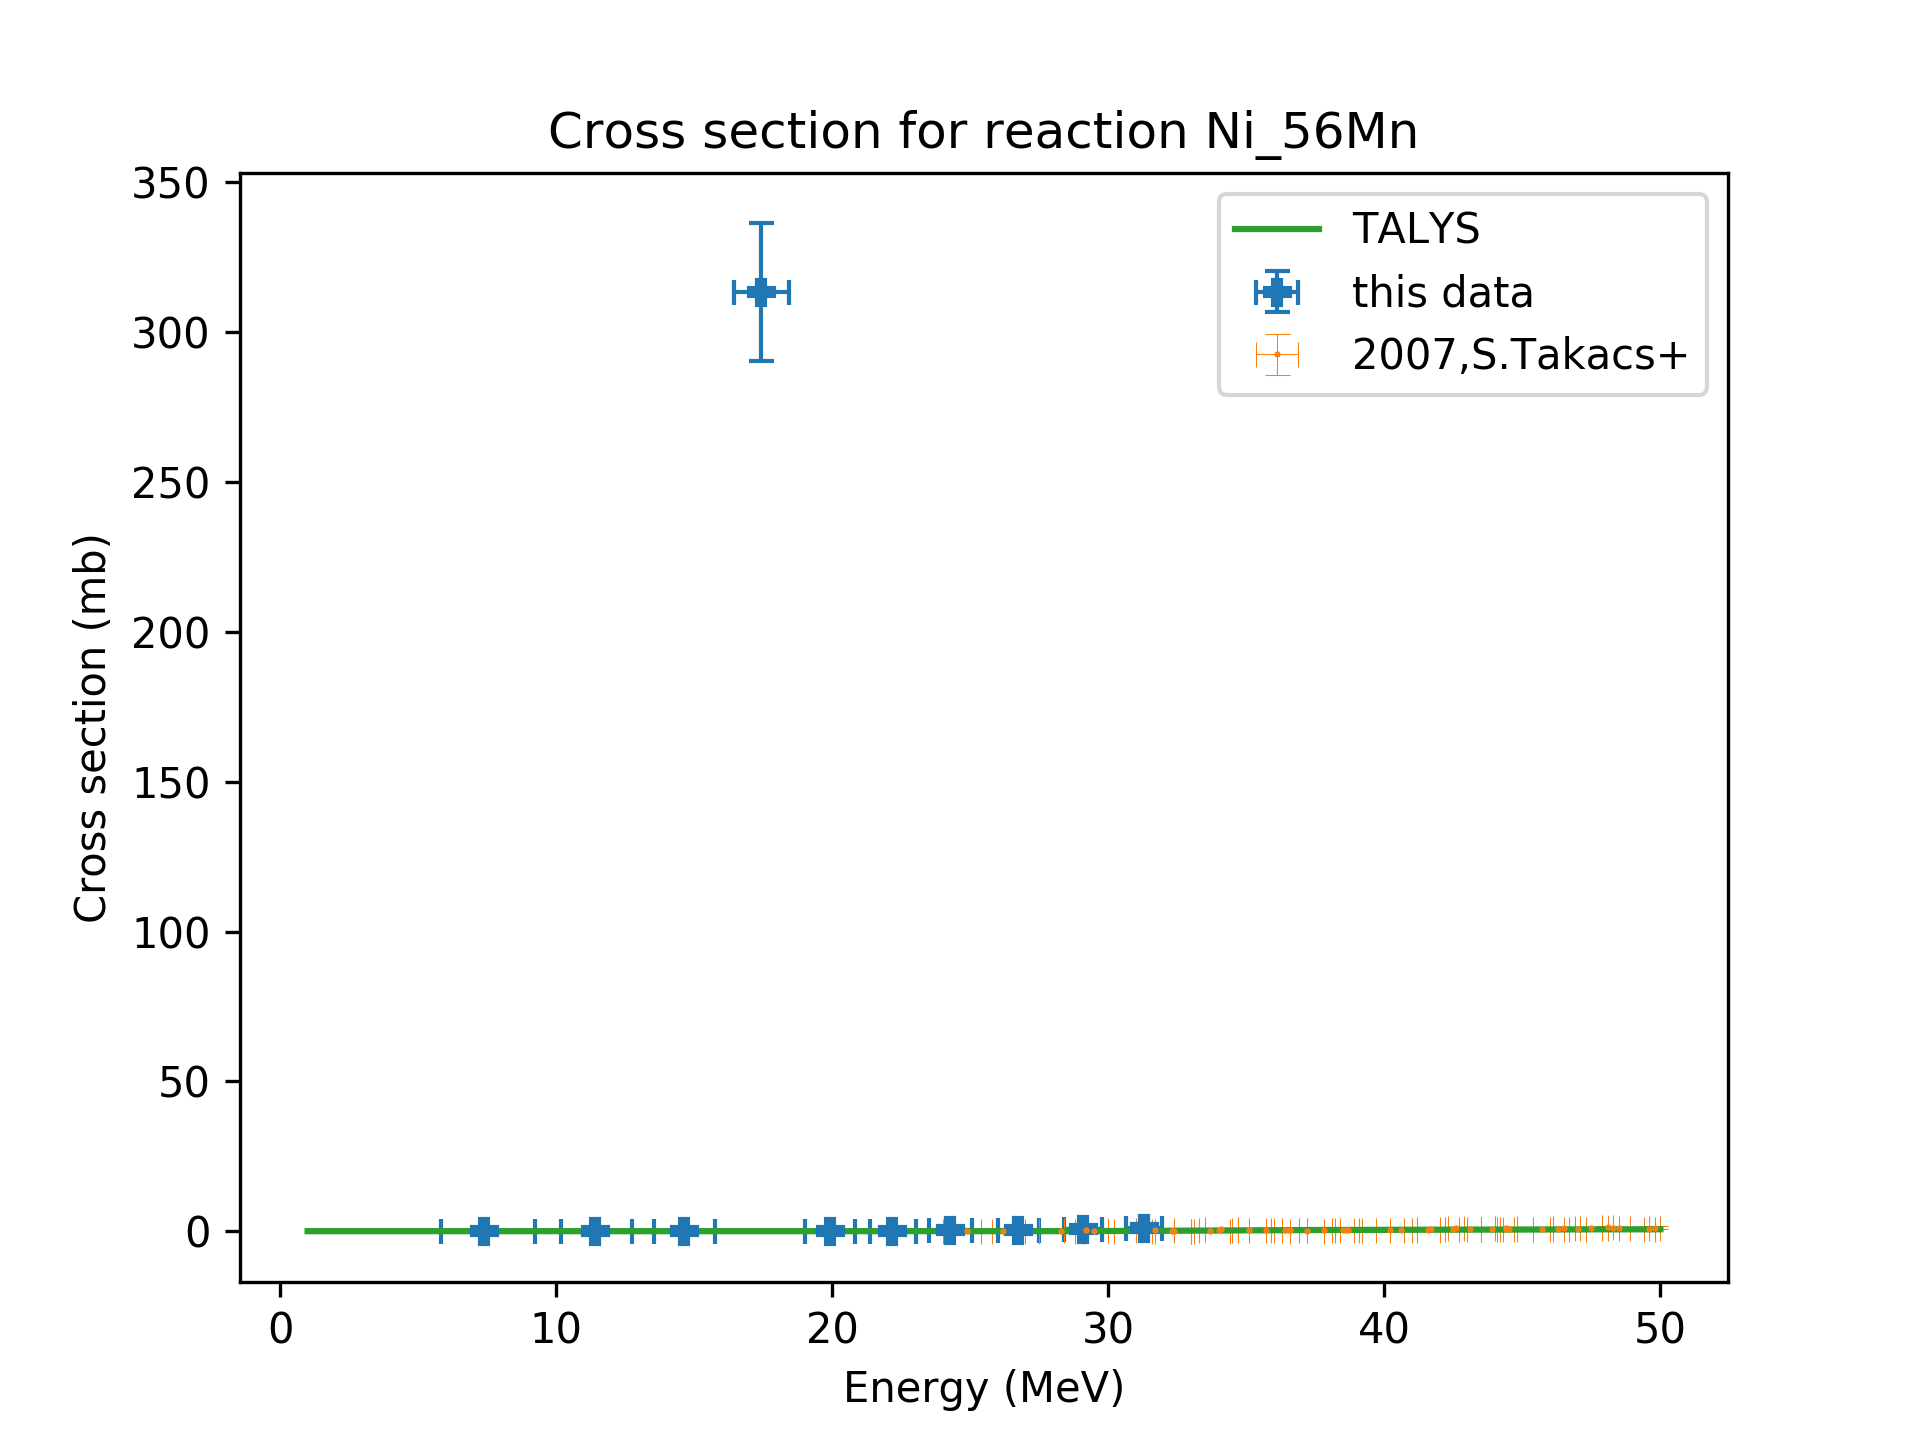
\includegraphics[width=5cm]{Results/Ni_56Mn.png} }}%
    \quad
    \subfloat[]{{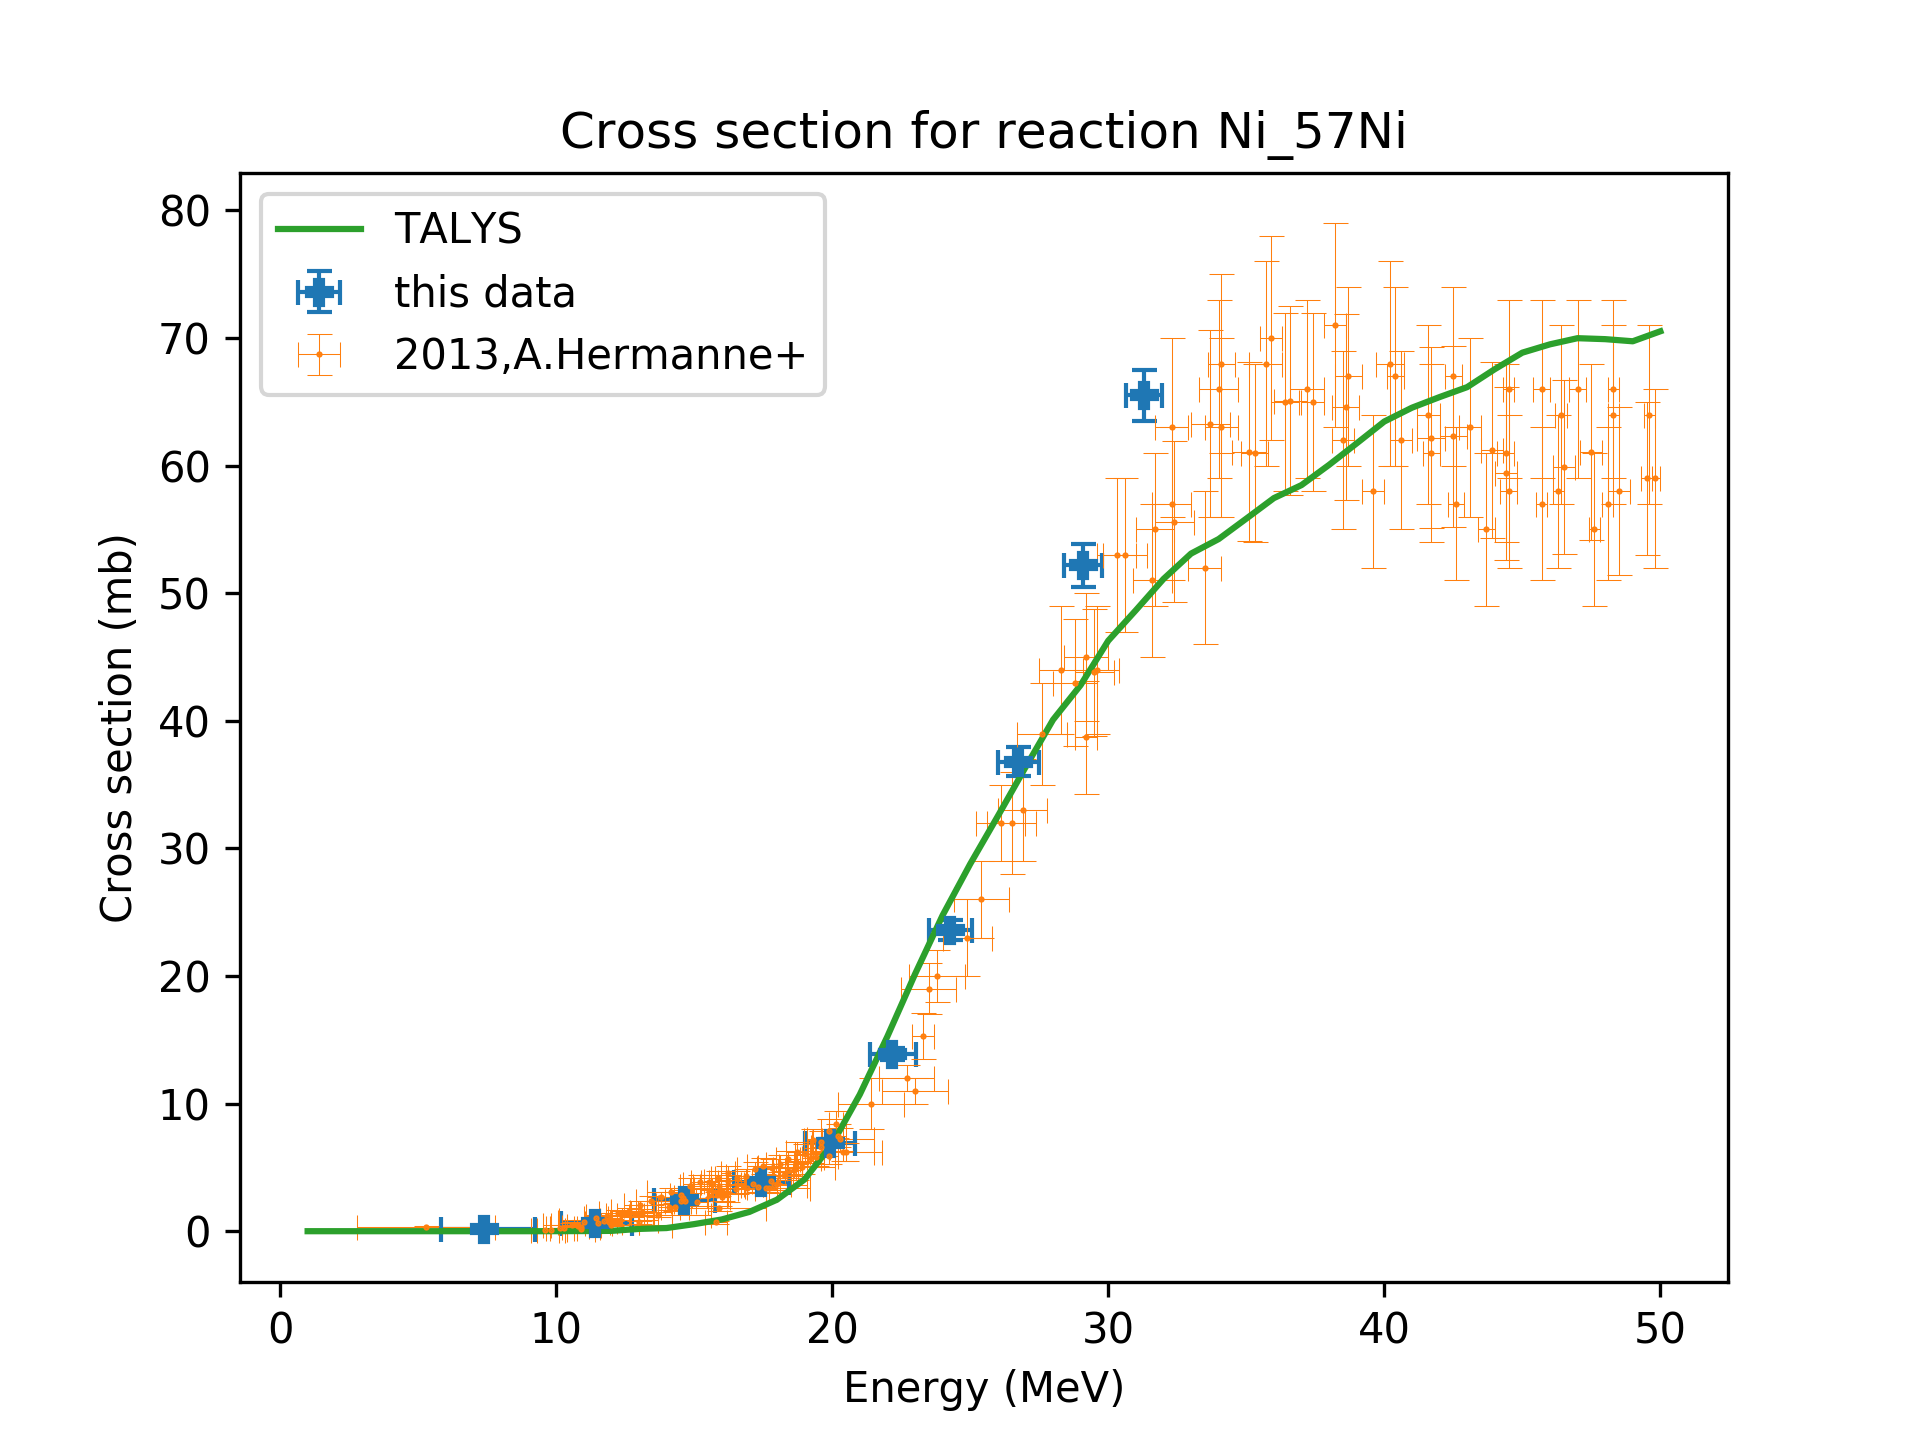
\includegraphics[width=5cm]{Results/Ni_57Ni.png} }}%
    \quad
    \caption{Nickel  }%
    \label{fig:Ni_crosssections}%
\end{figure}

\section{Cupper cross sections}

\begin{figure}%
    \centering
    \subfloat[]{{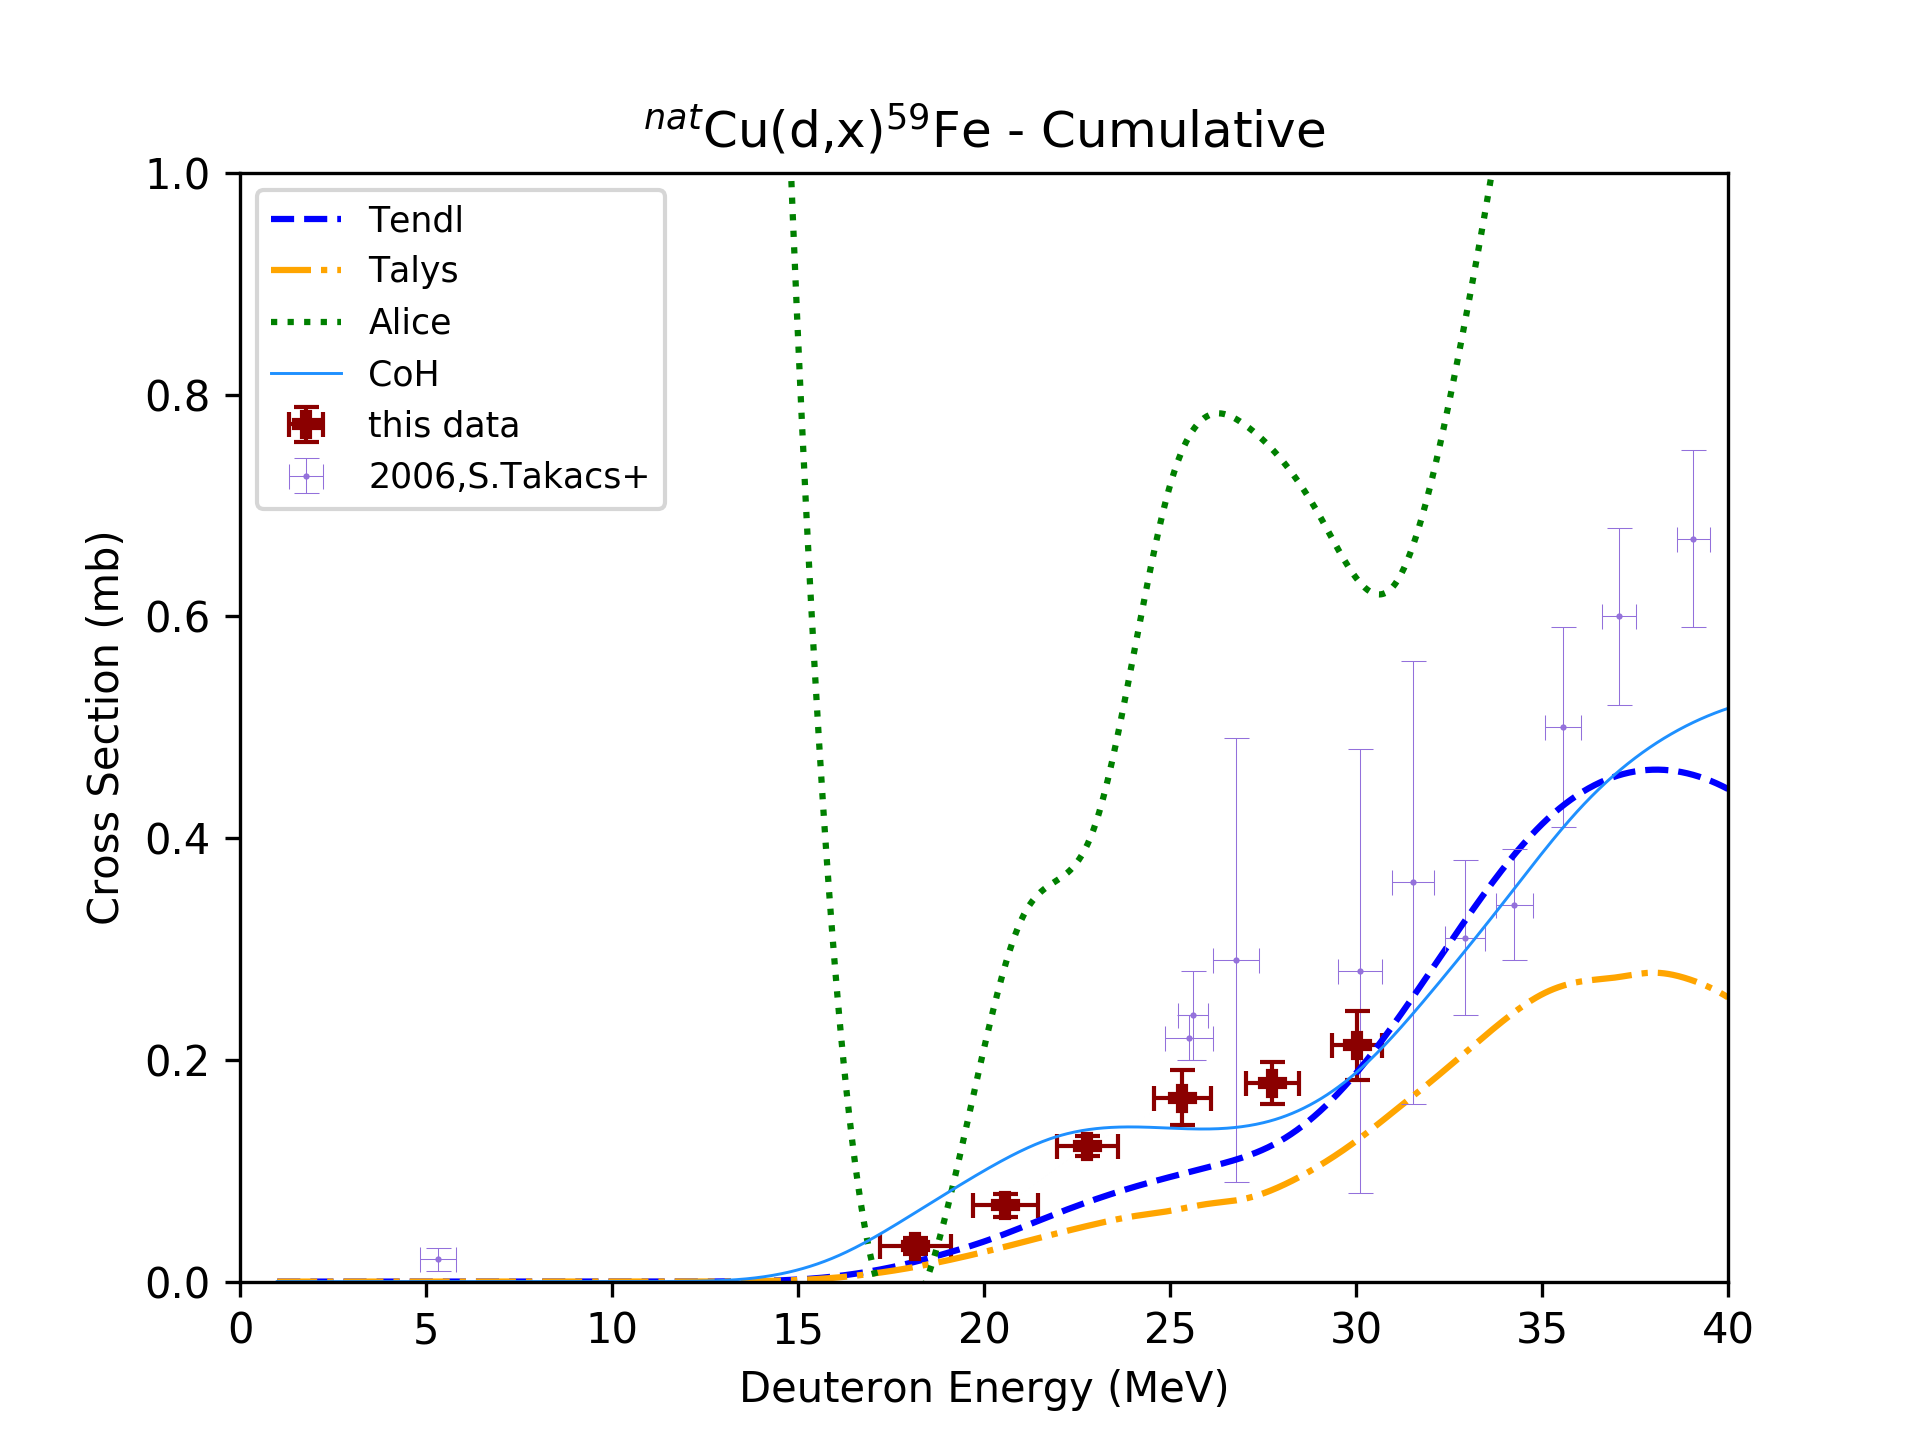
\includegraphics[width=5cm]{Results/Cu_59Fe.png}}%
    \quad
    \subfloat[]{{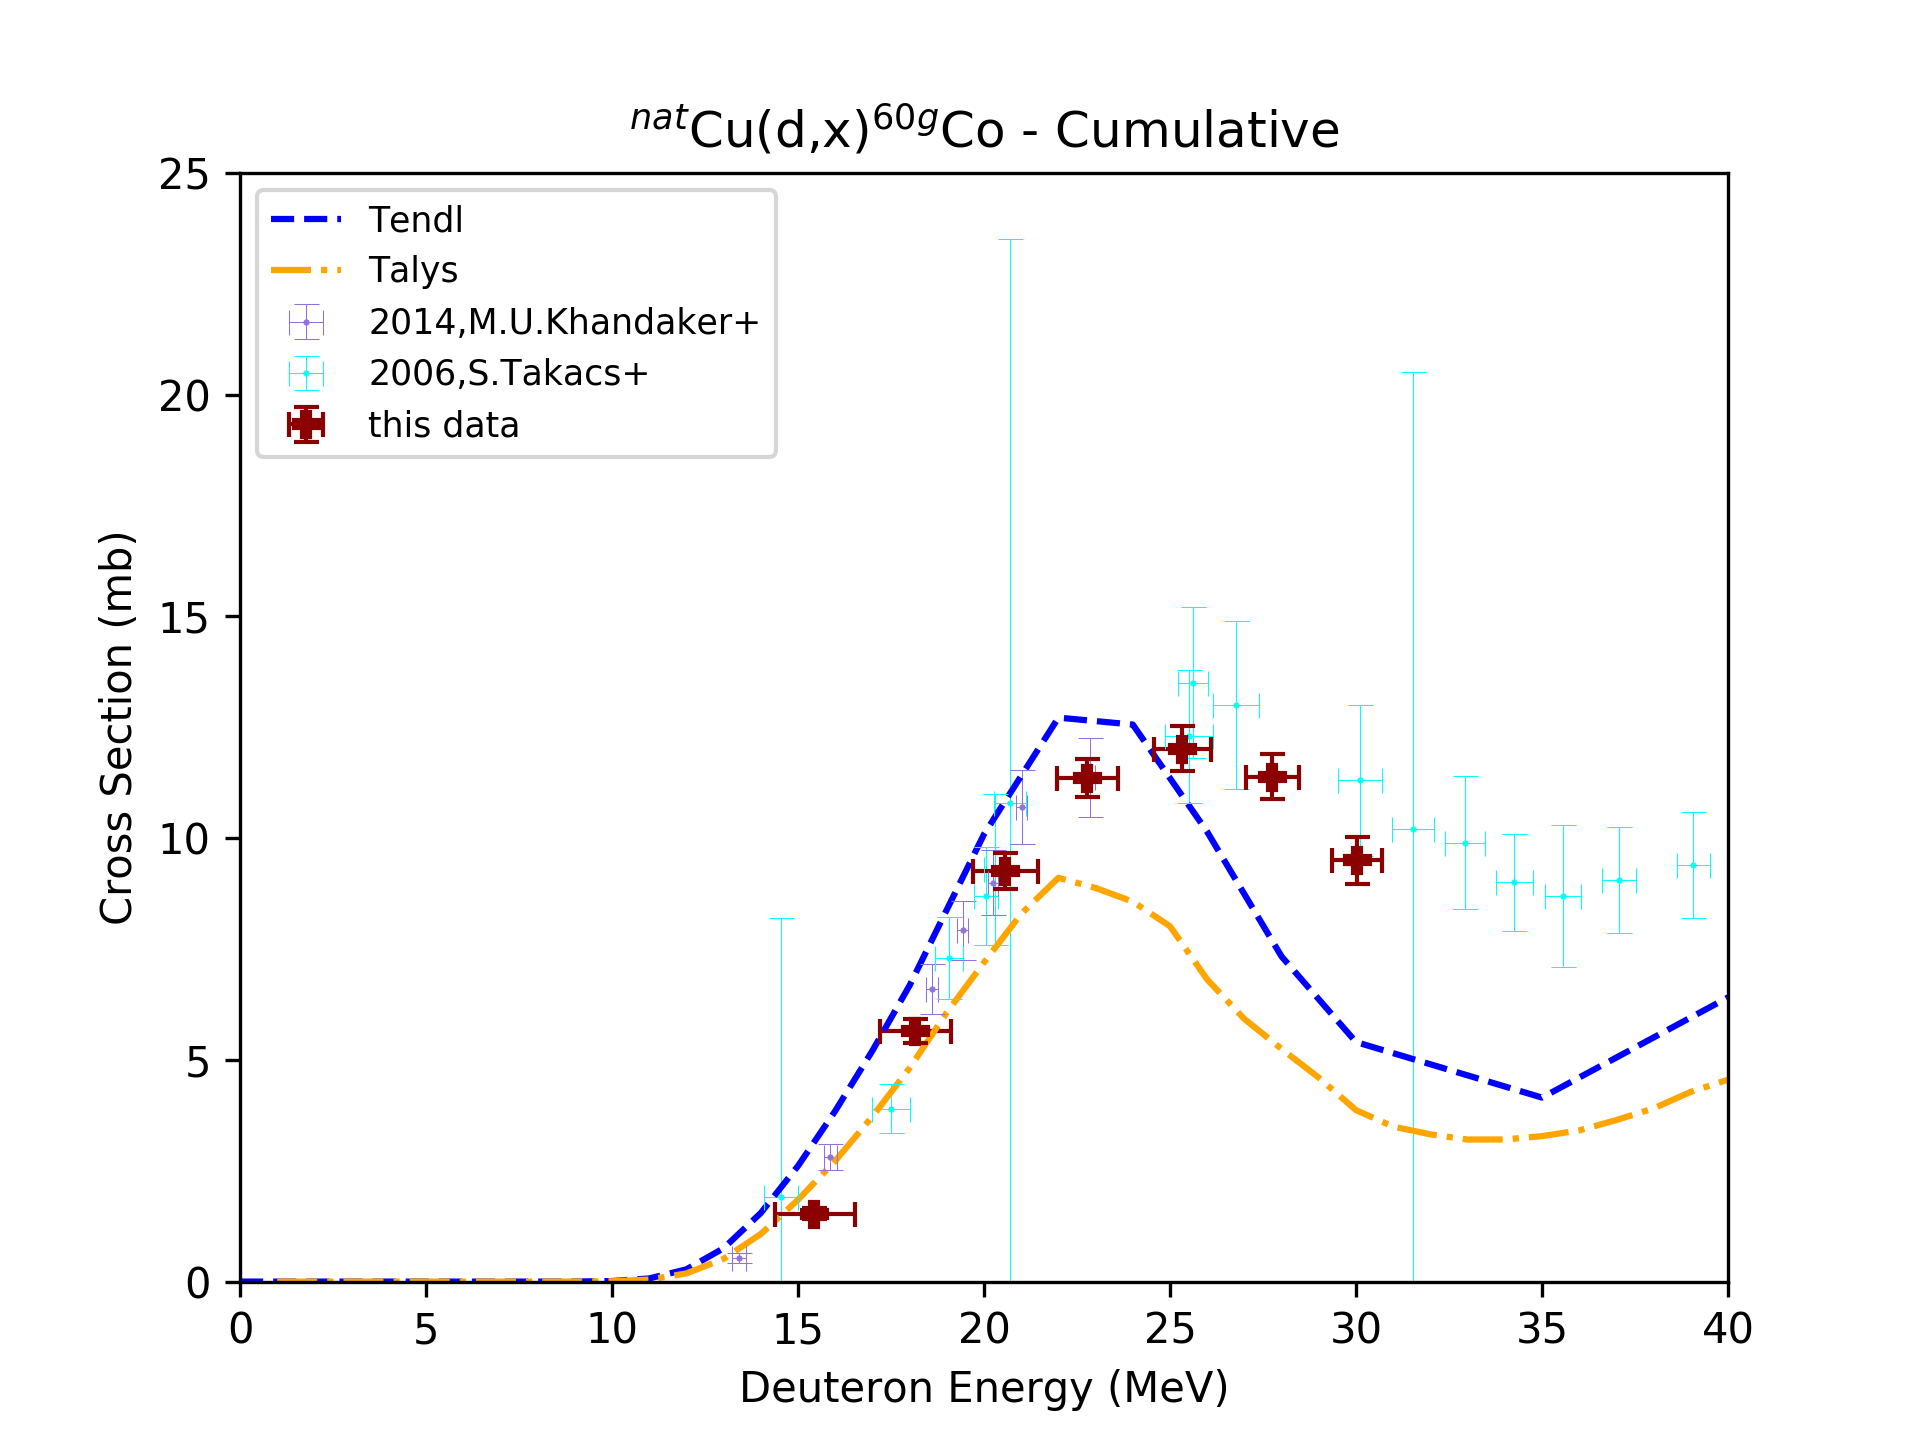
\includegraphics[width=5cm]{Results/Cu_60Co.png} }}%
    \subfloat[]{{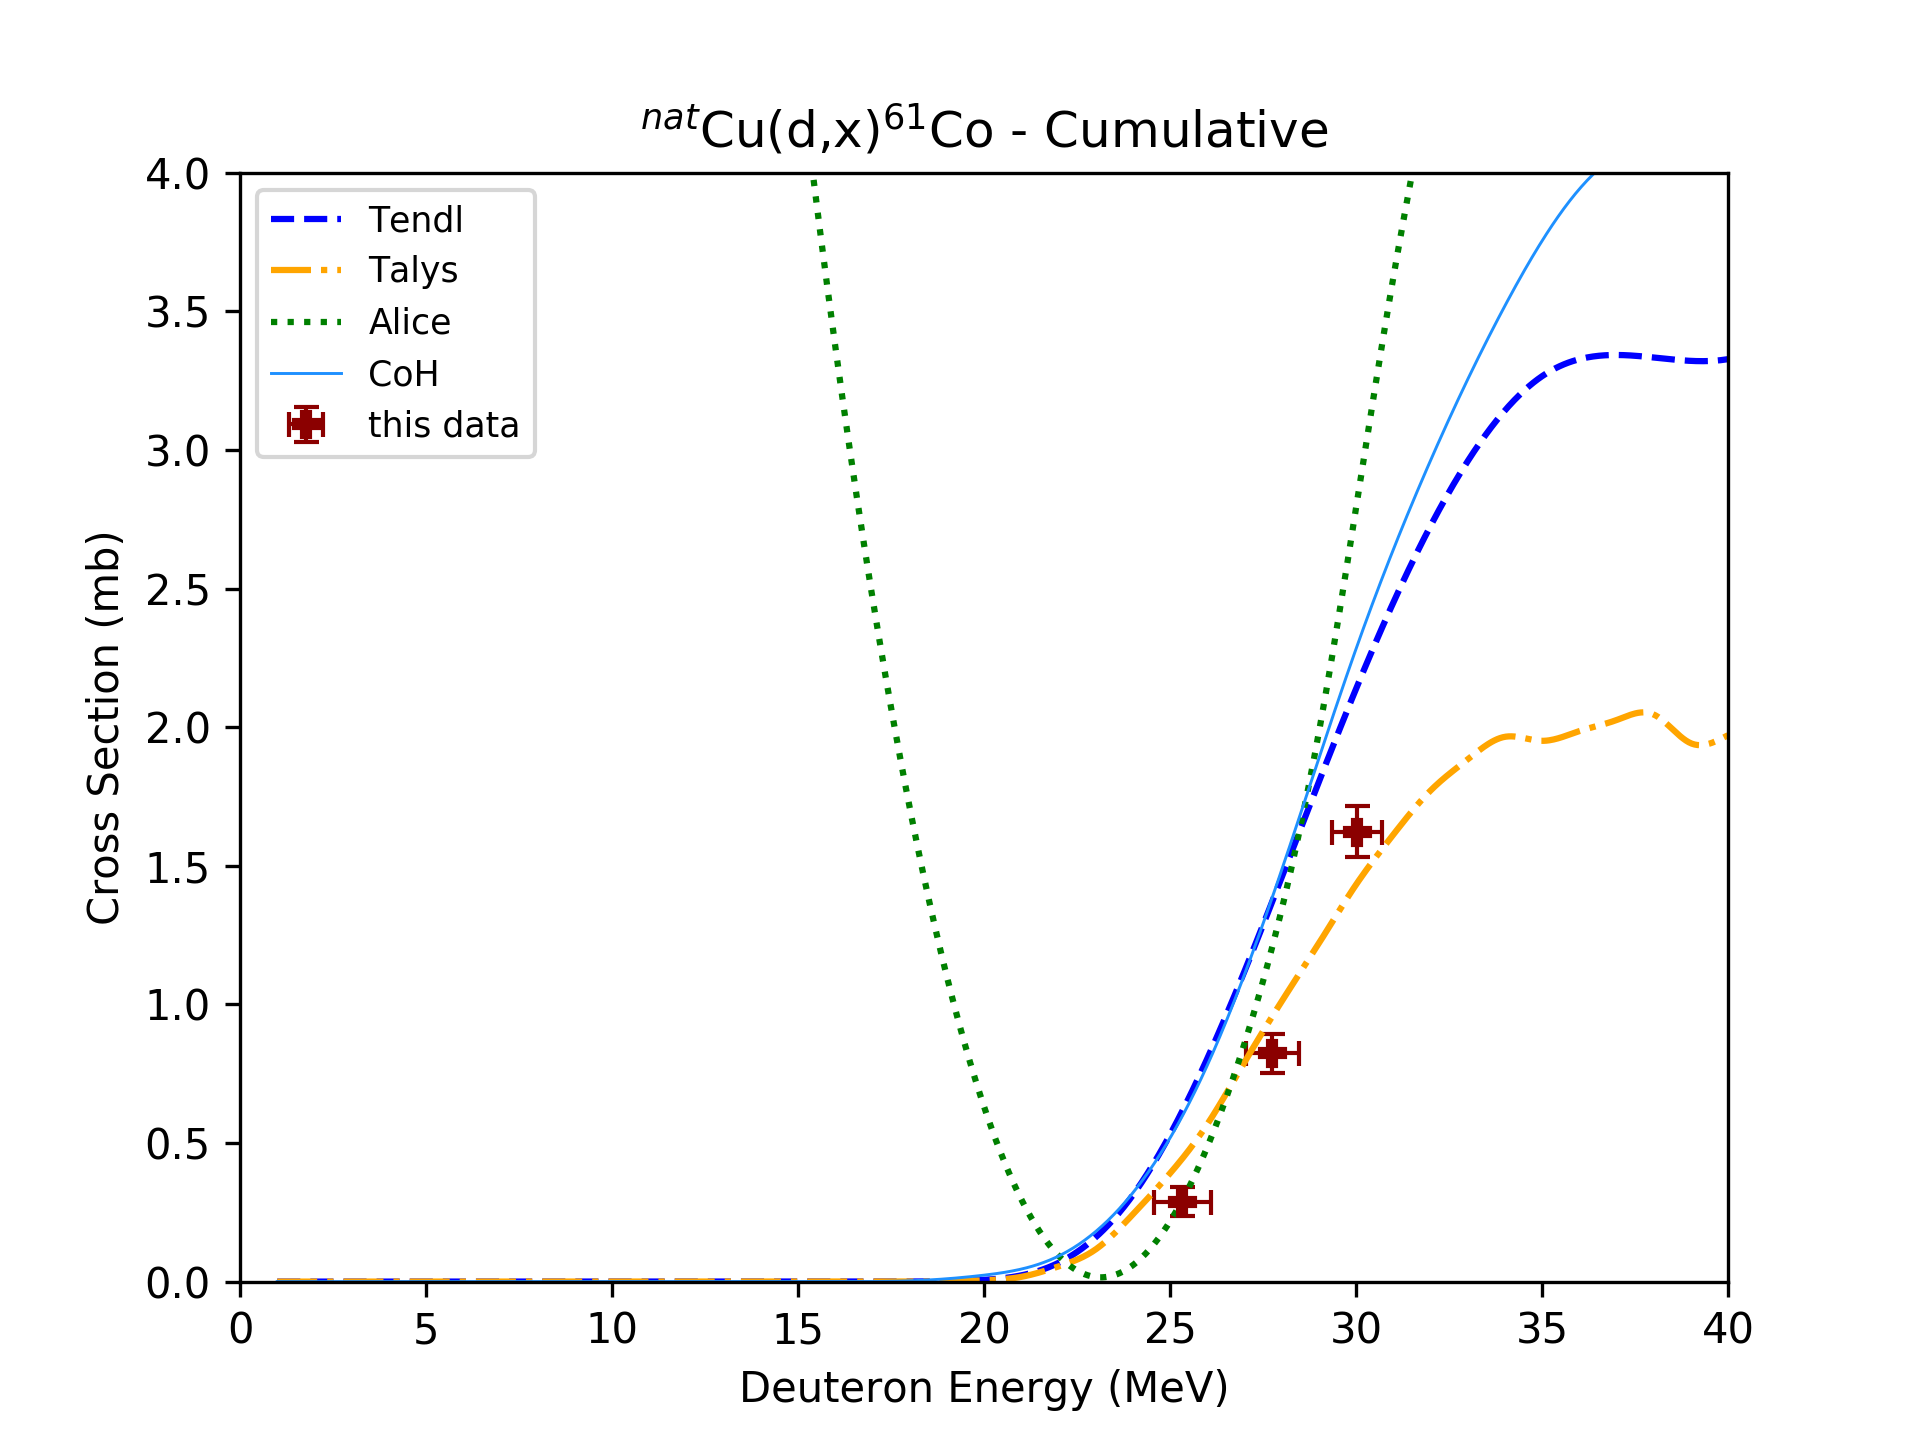
\includegraphics[width=5cm]{Results/Cu_61Co.png} }}%
    \quad
    \subfloat[]{{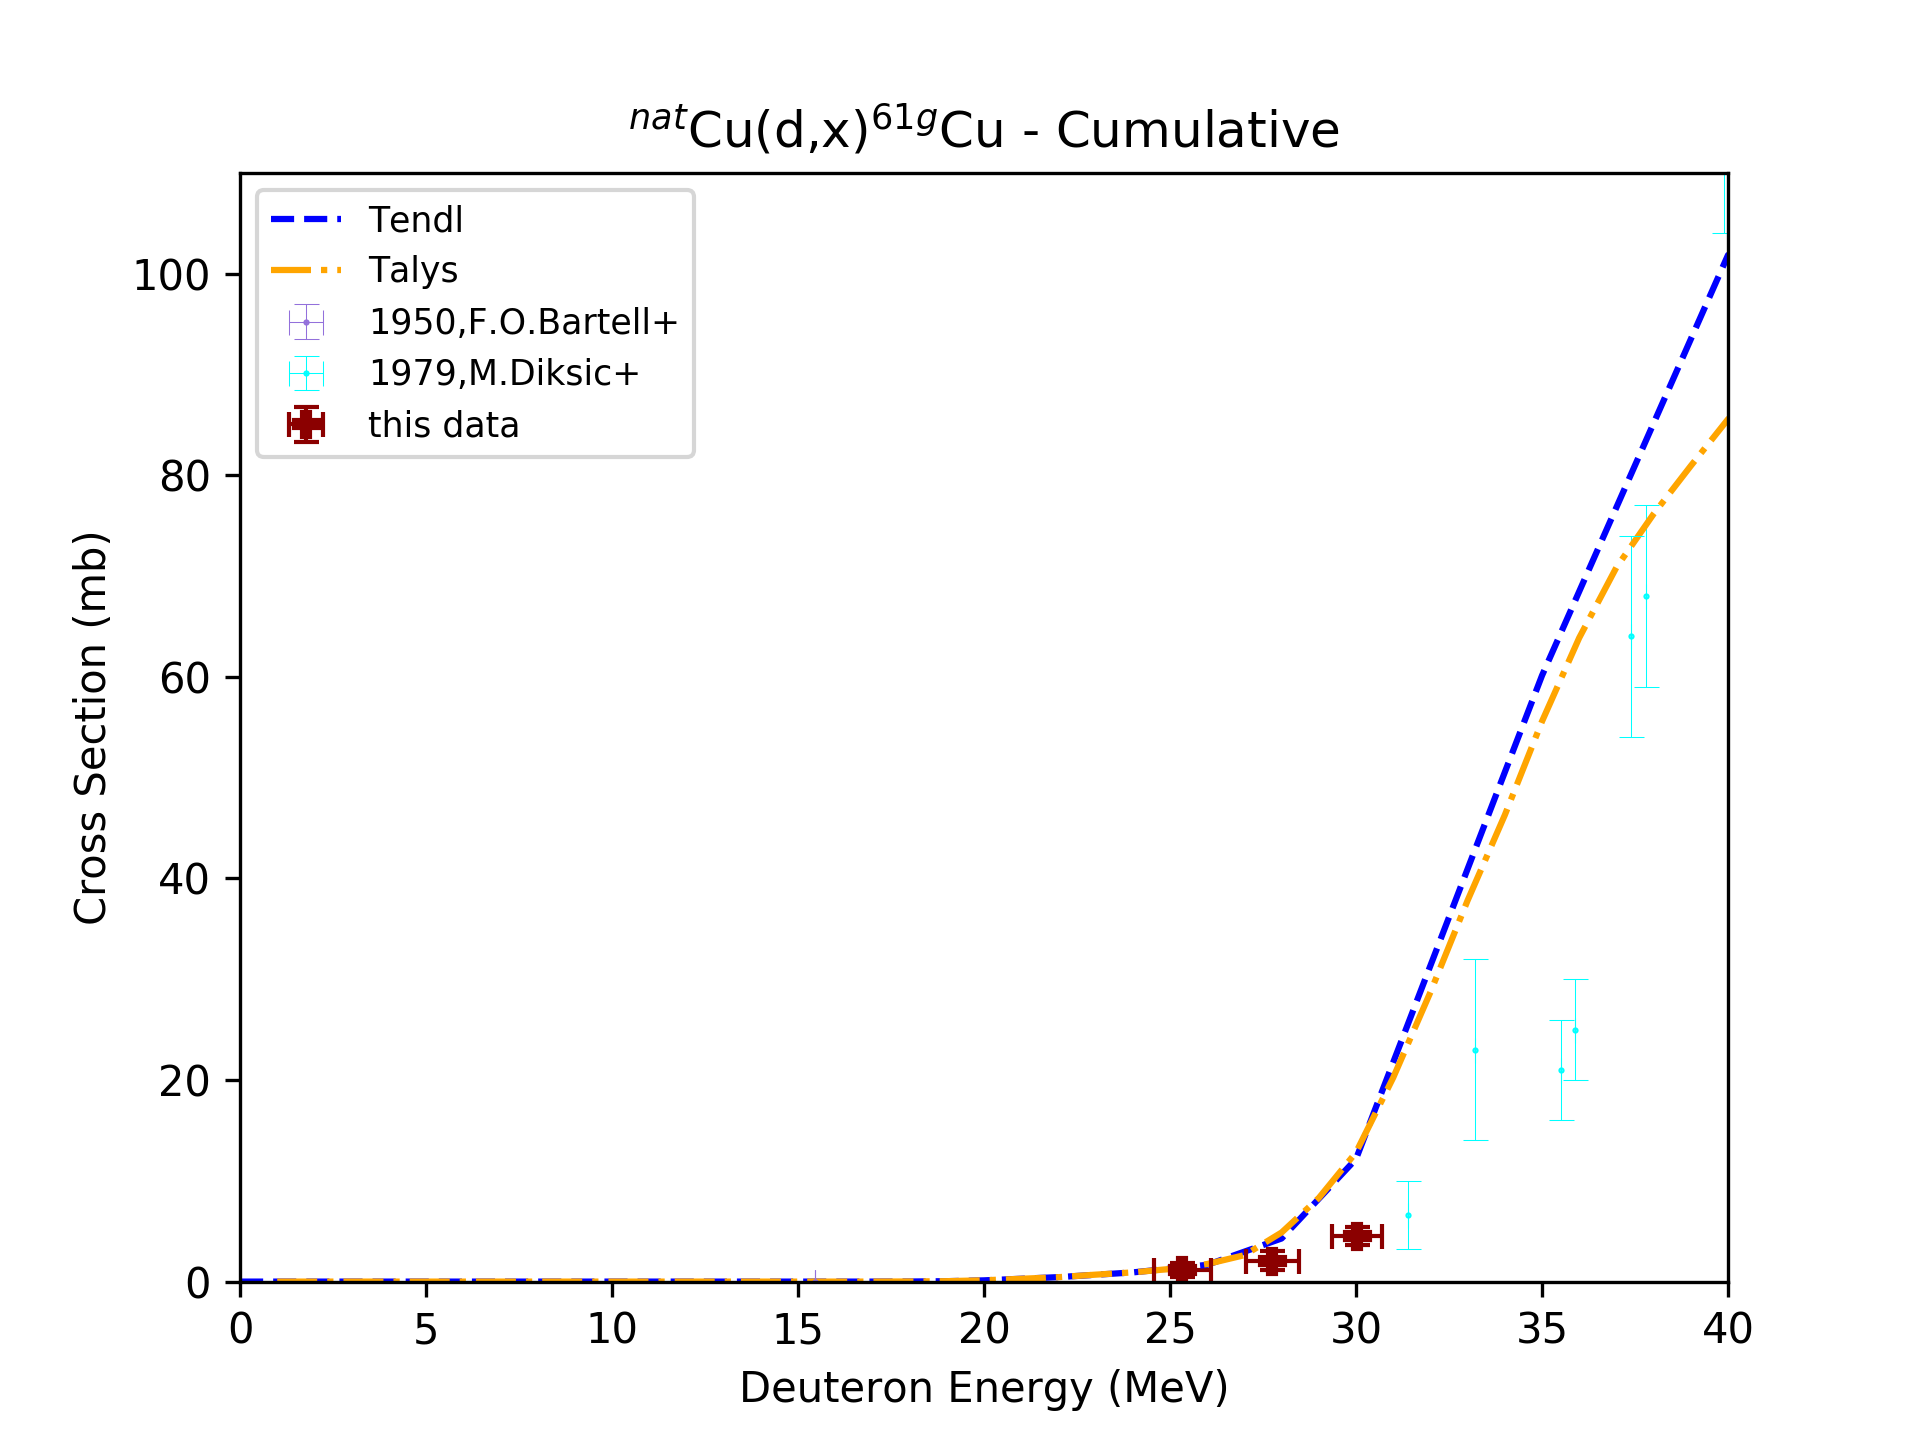
\includegraphics[width=5cm]{Results/Cu_61Cu.png} }}%
    \quad
    \subfloat[]{{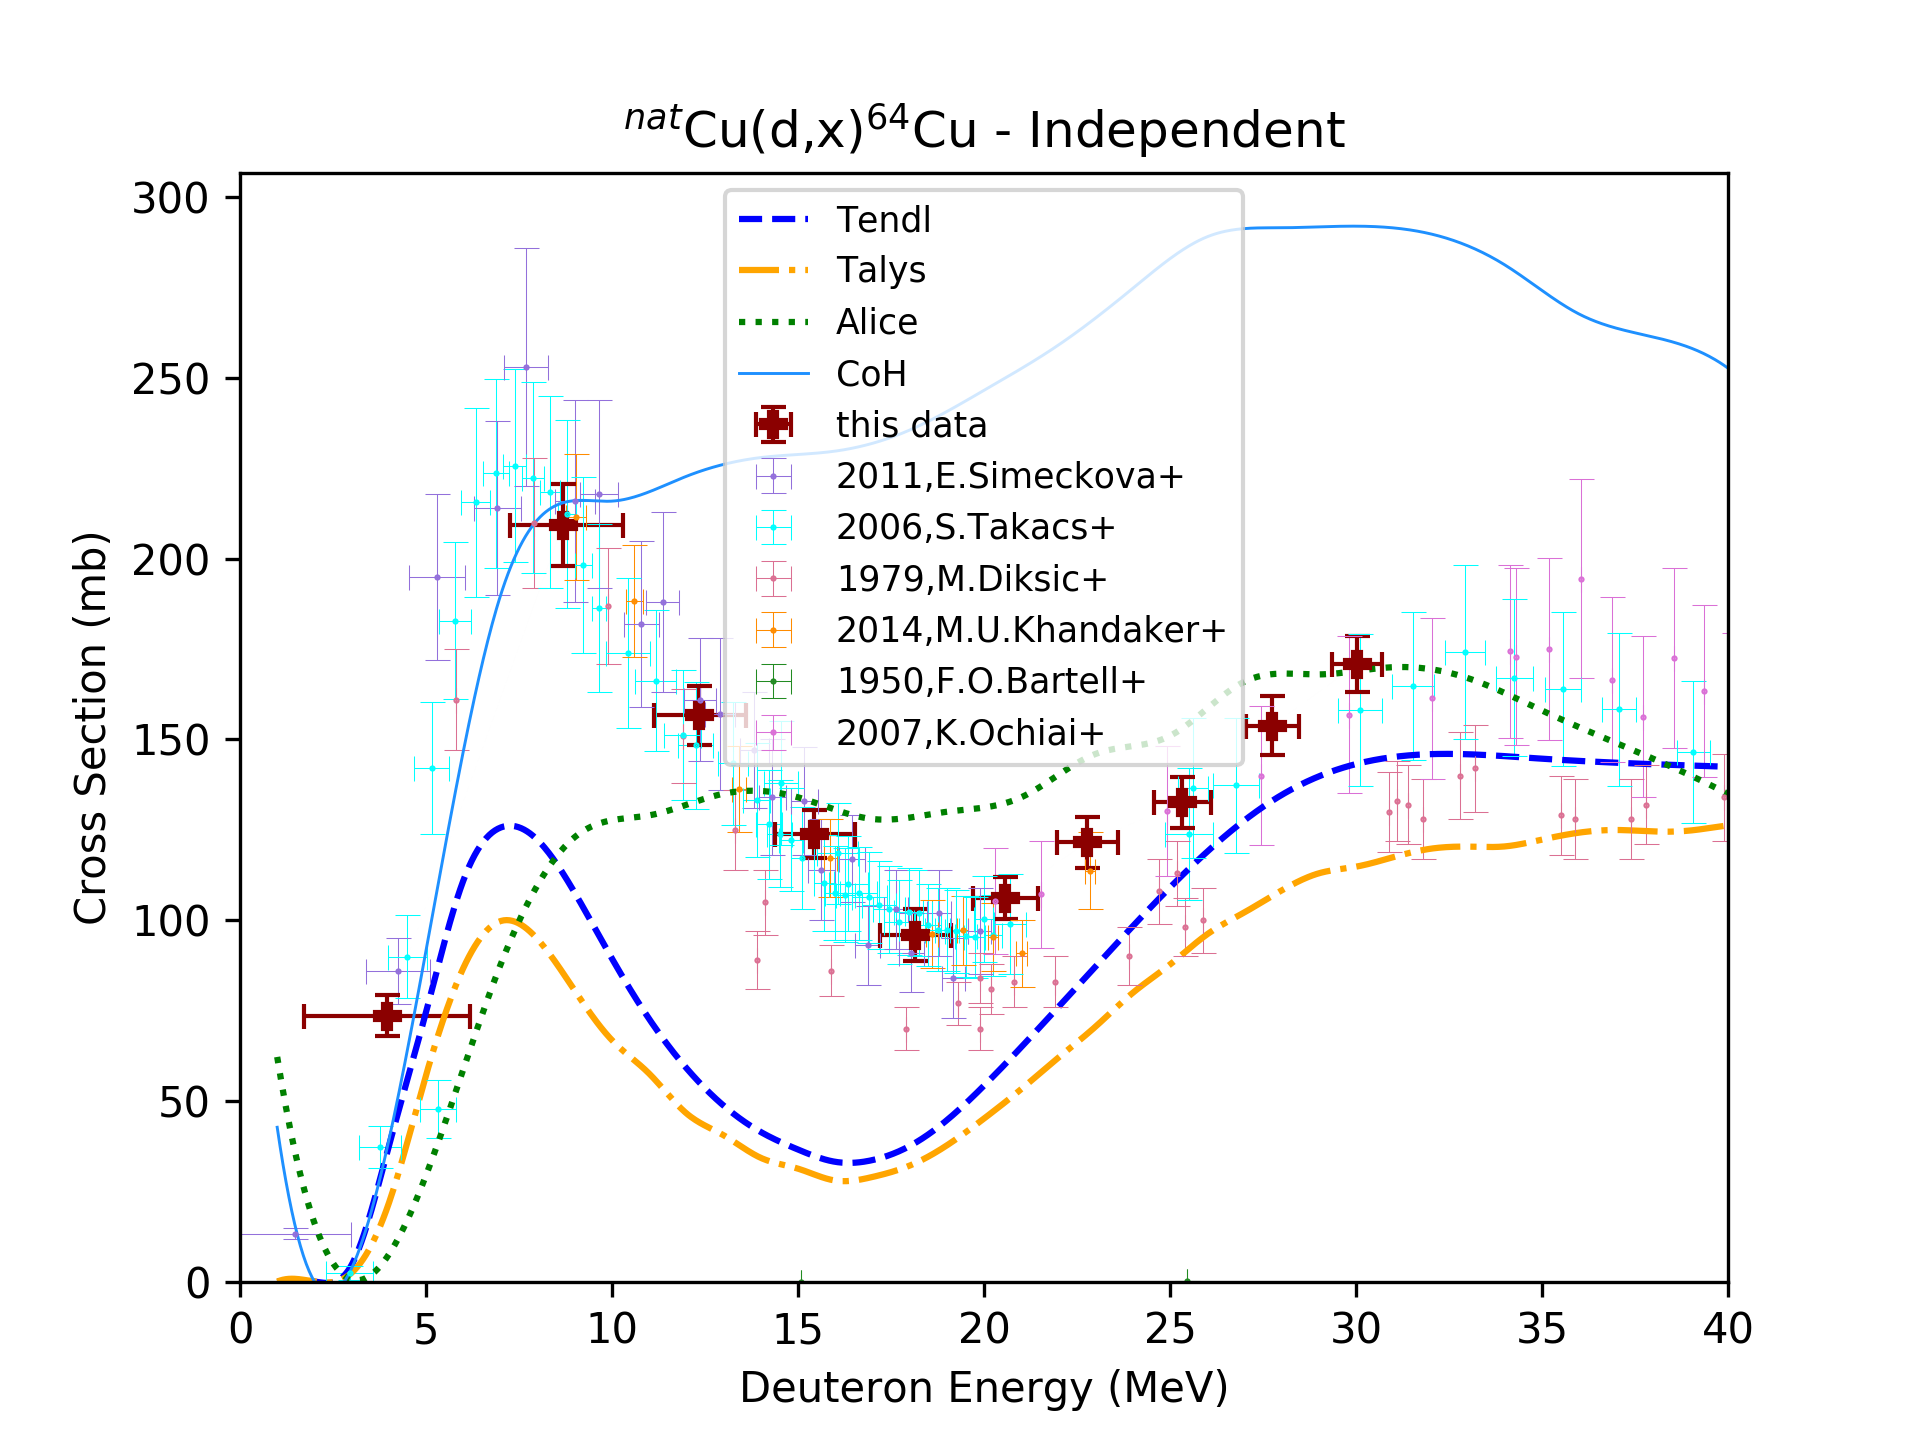
\includegraphics[width=5cm]{Results/Cu_64Cu.png} }}%
    \quad
    \subfloat[caption]{{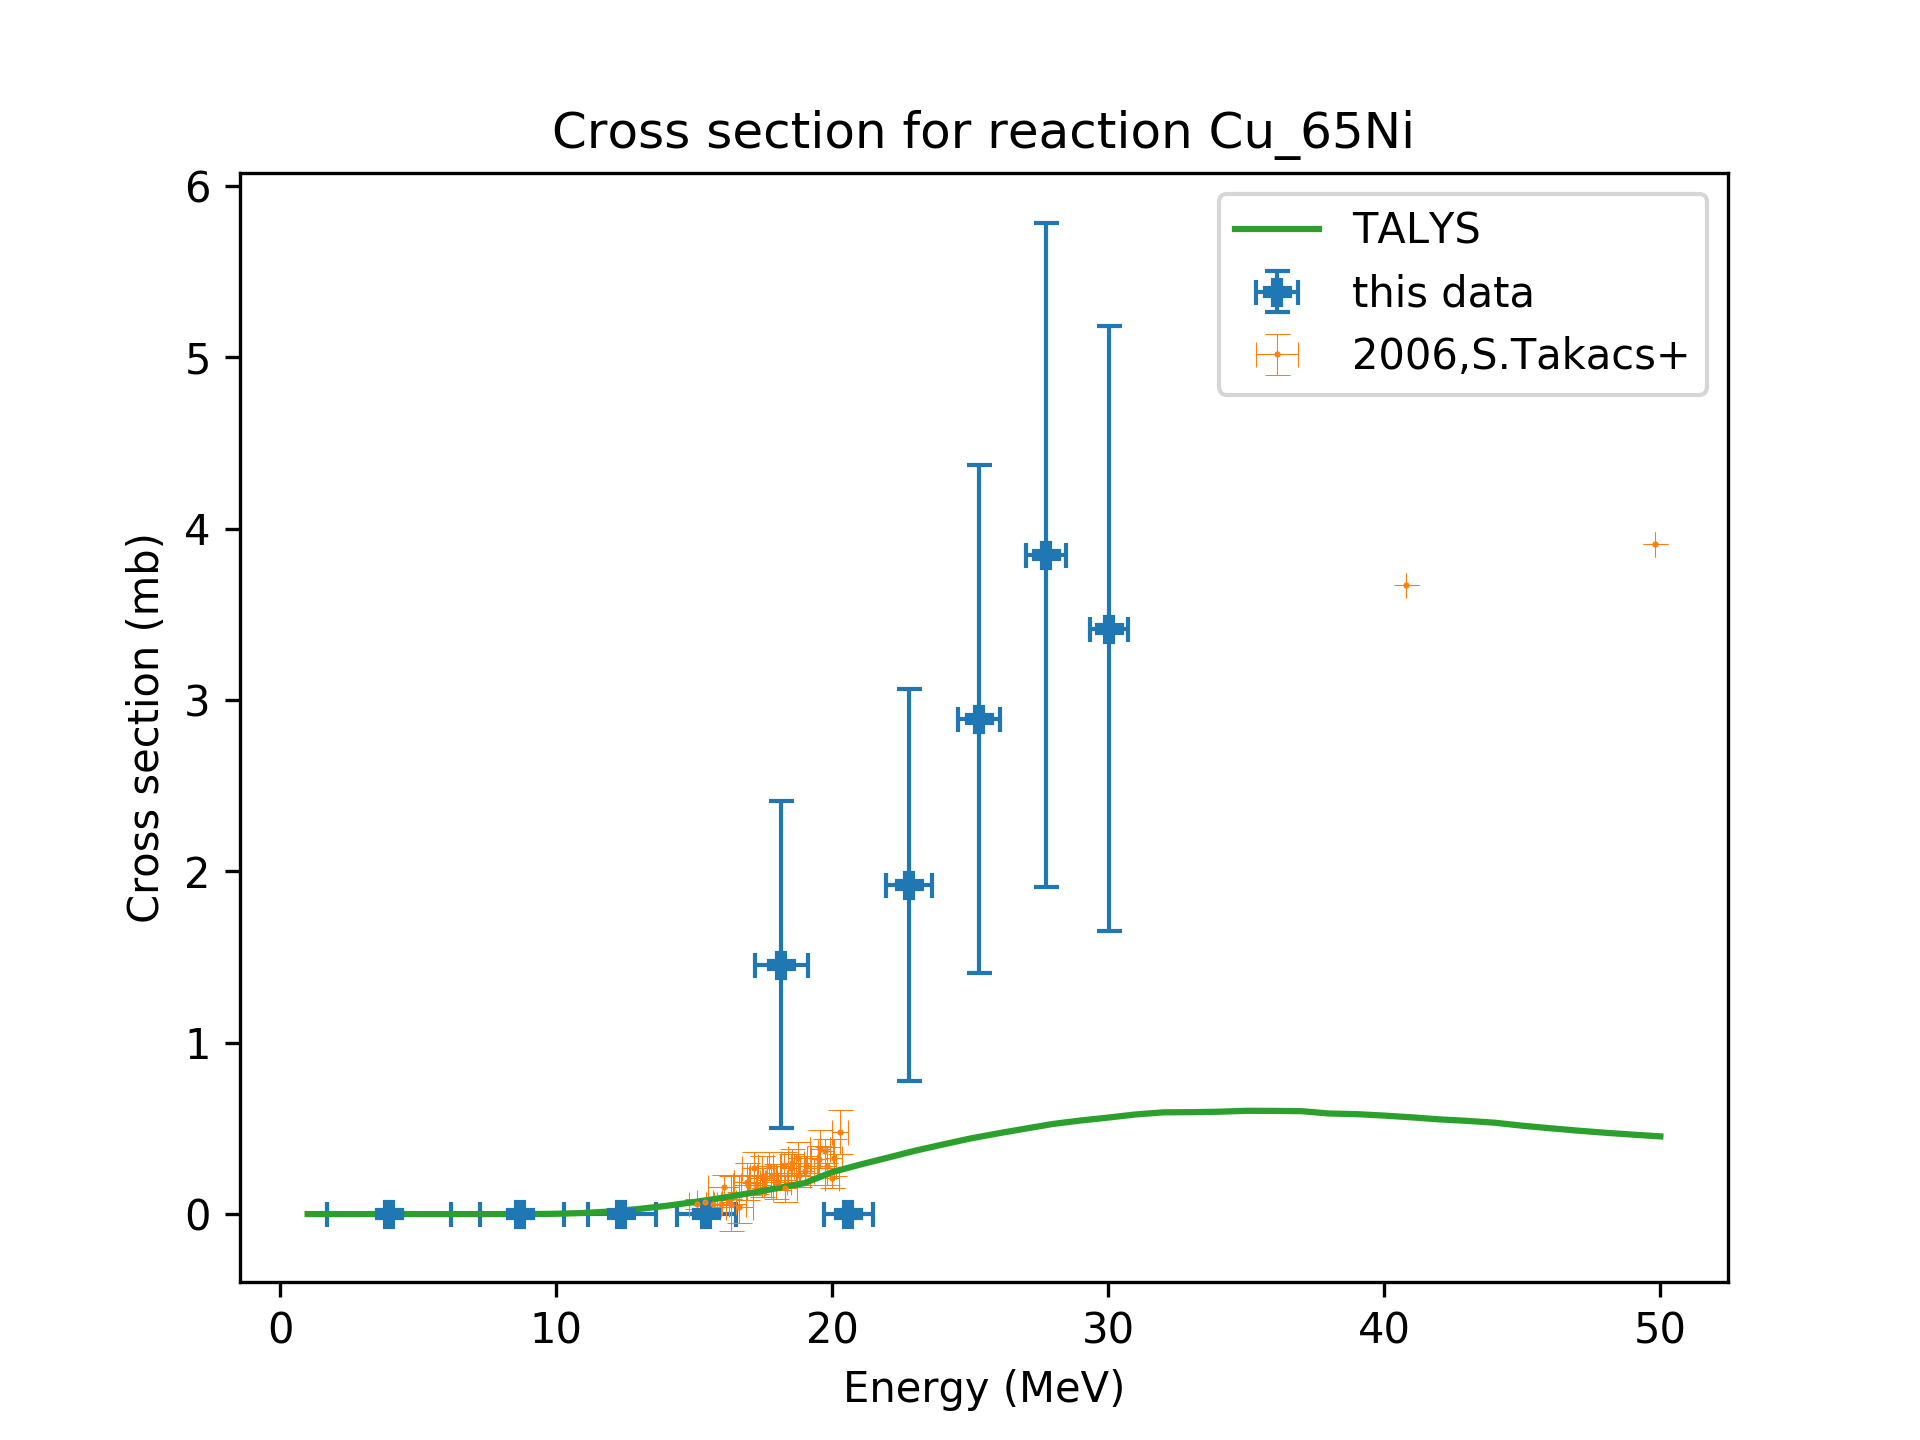
\includegraphics[width=5cm]{Results/Cu_65Ni.png} }}%
    \quad
    \caption{Cupper cross sections  }%
    \label{fig:Cu_crosssections}%
\end{figure}

\section{Iron cross sections}

\begin{figure}%
    \centering
    \subfloat[]{{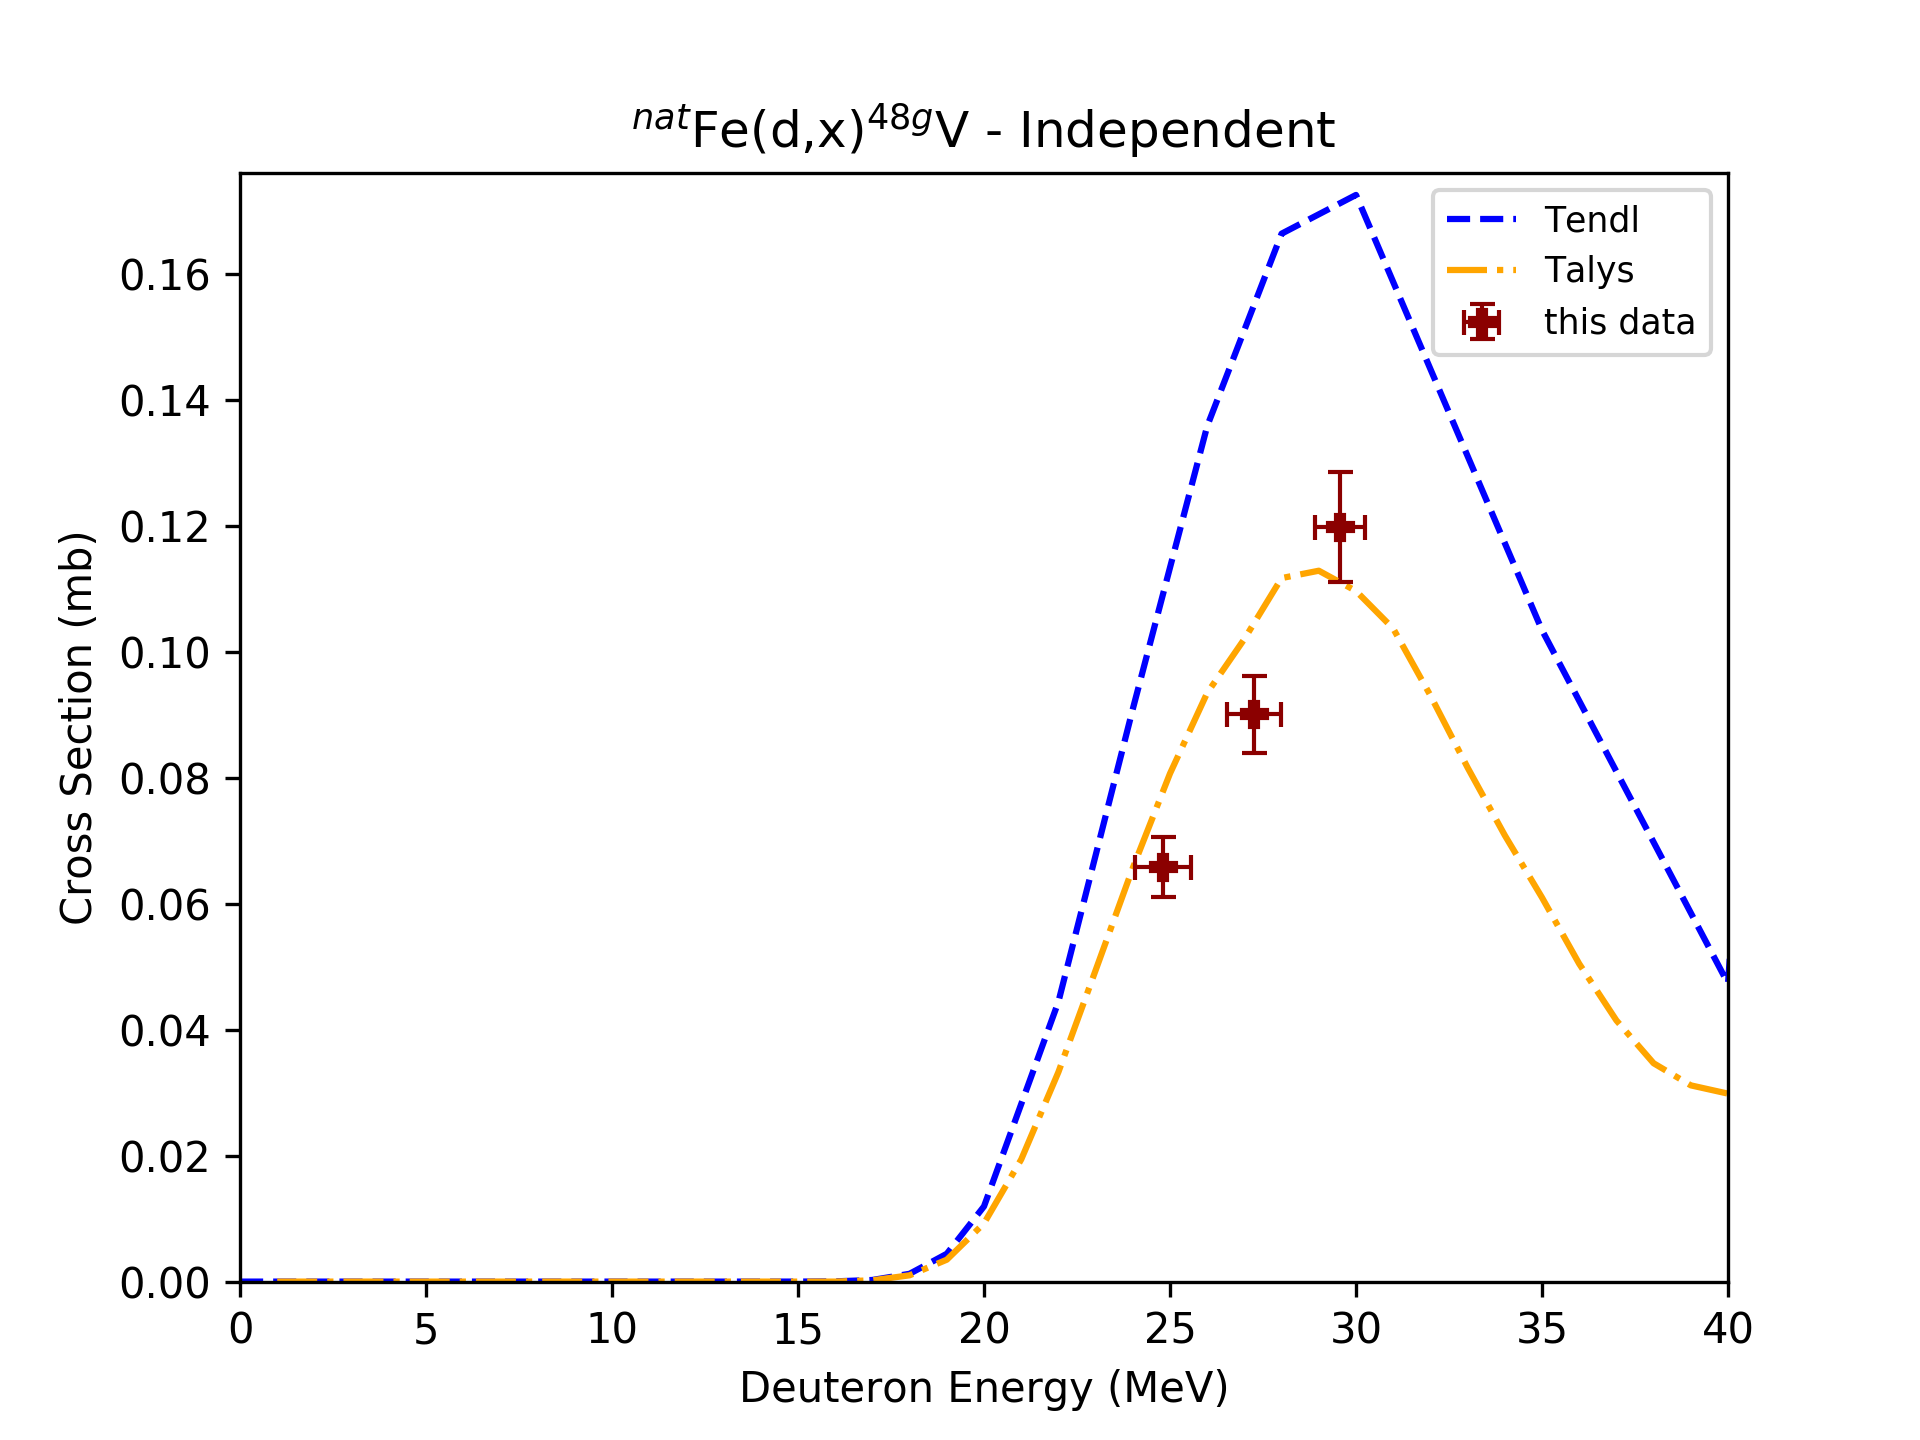
\includegraphics[width=5cm]{Results/Fe_48V.png}}%
    \quad
    \subfloat[]{{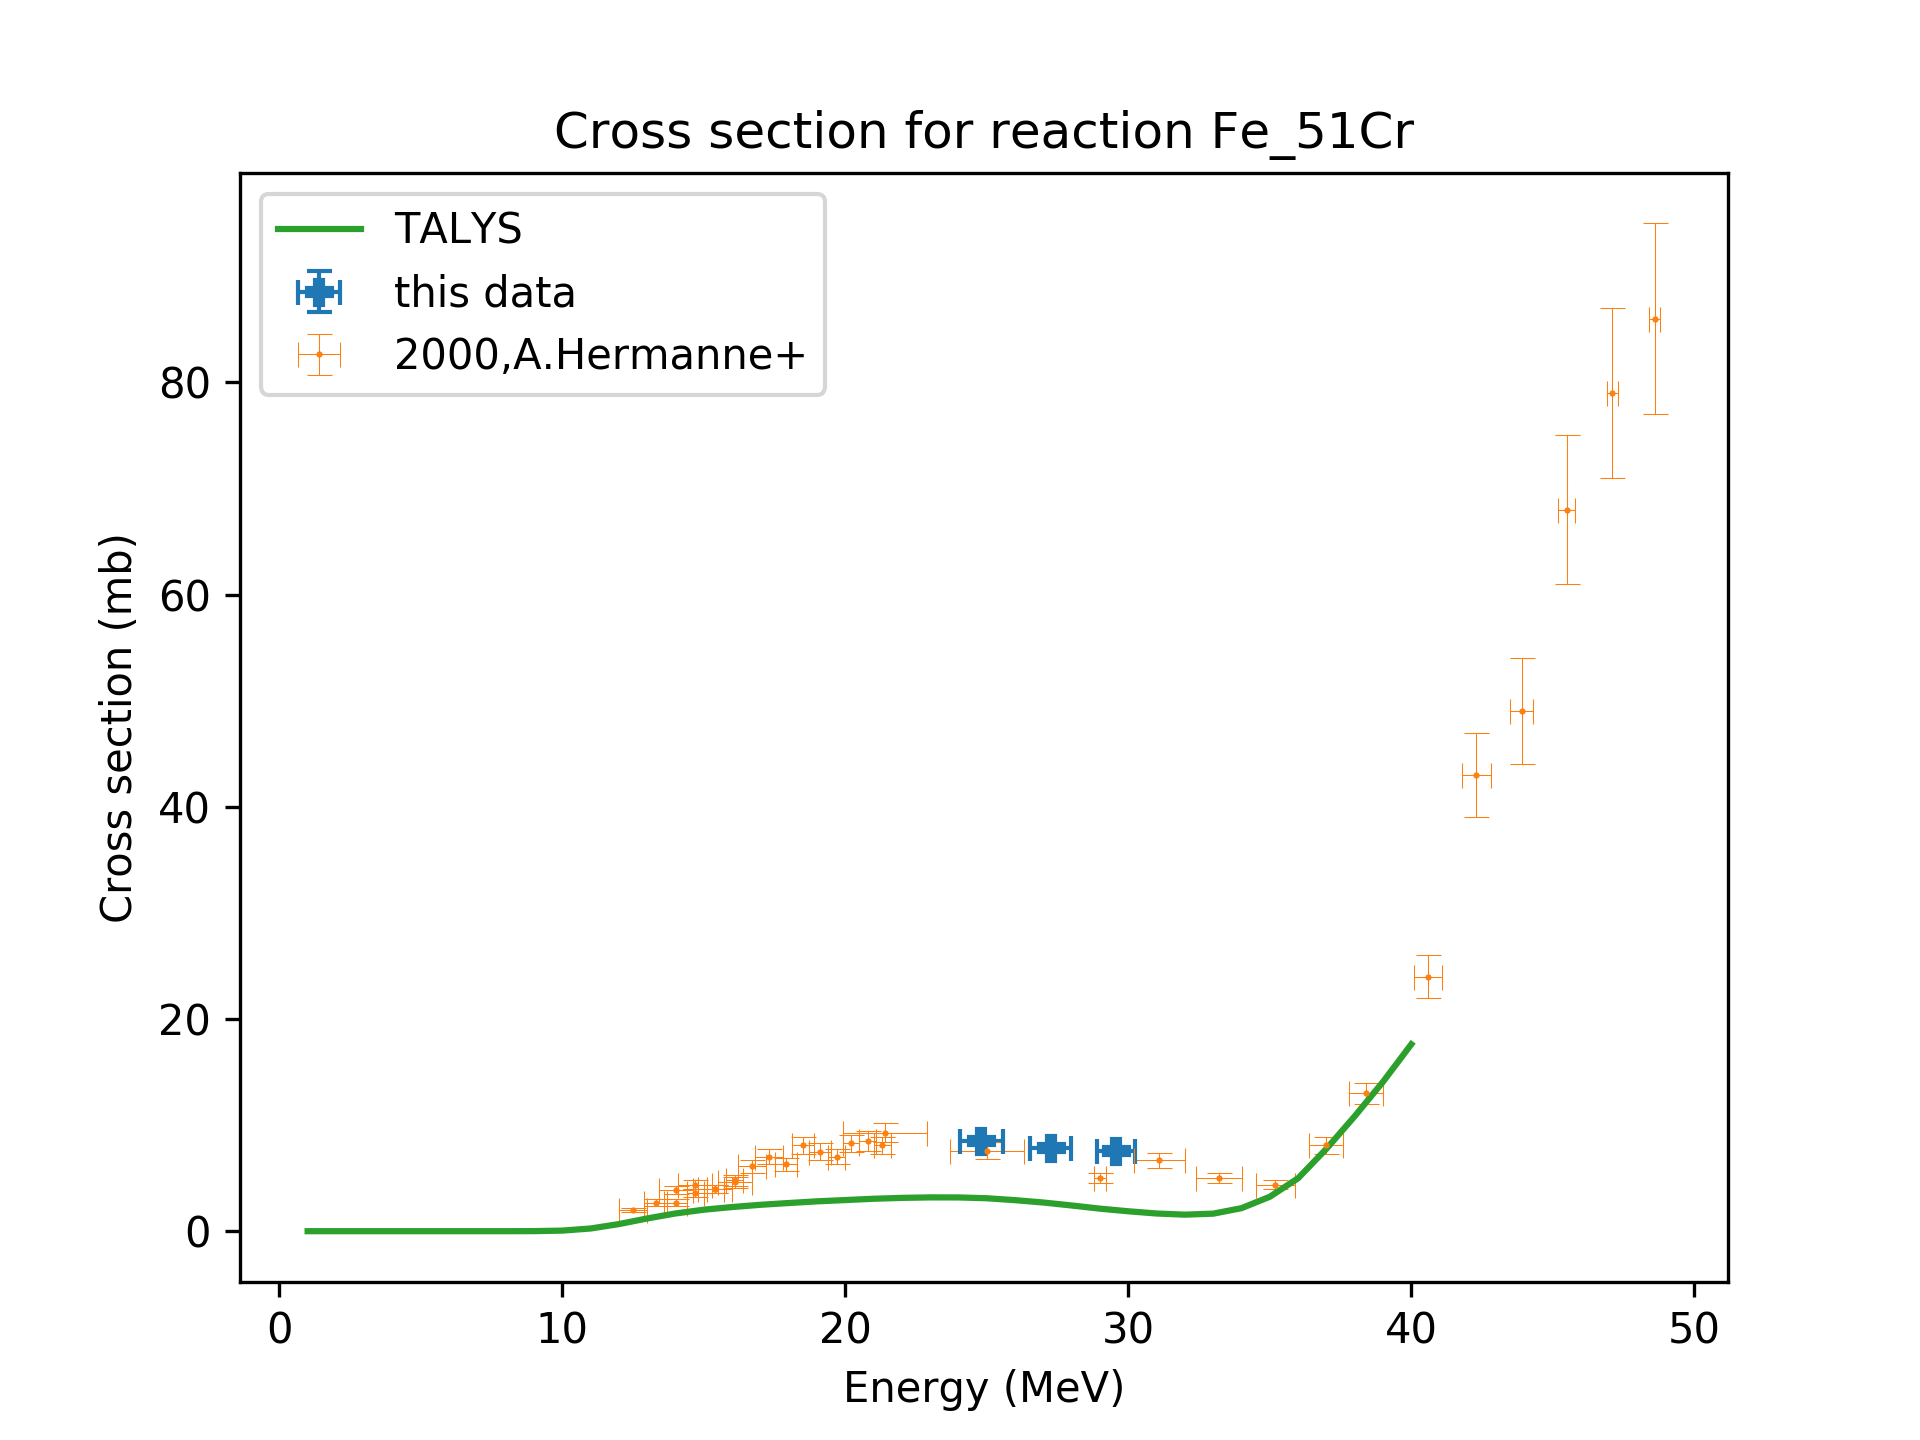
\includegraphics[width=5cm]{Results/Fe_51Cr.png} }}%
    \subfloat[]{{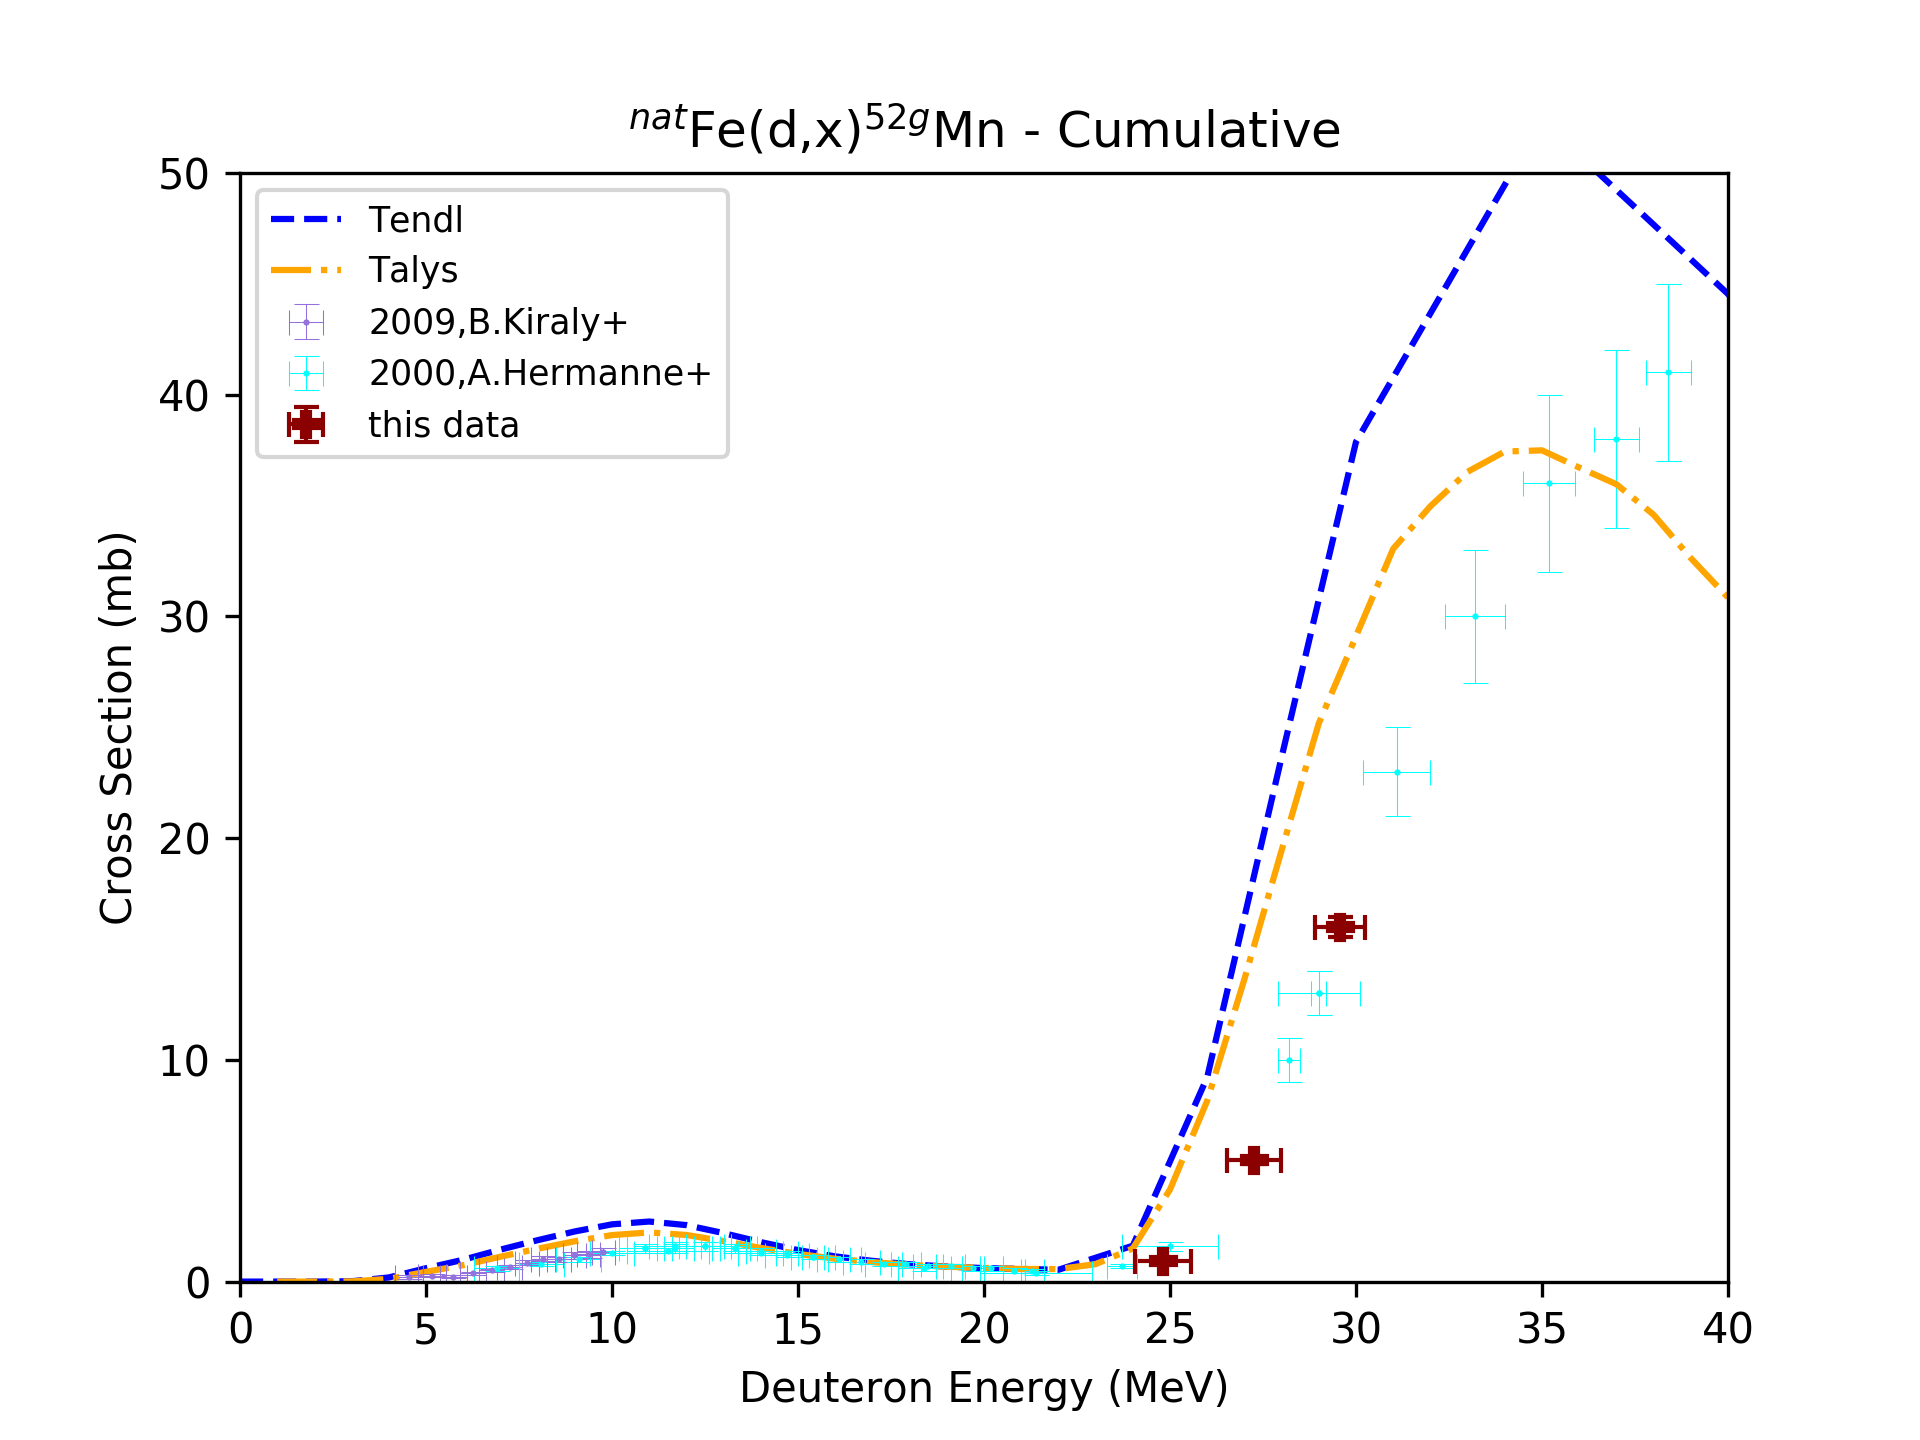
\includegraphics[width=5cm]{Results/Fe_52Mn.png} }}%
    \quad
    \subfloat[]{{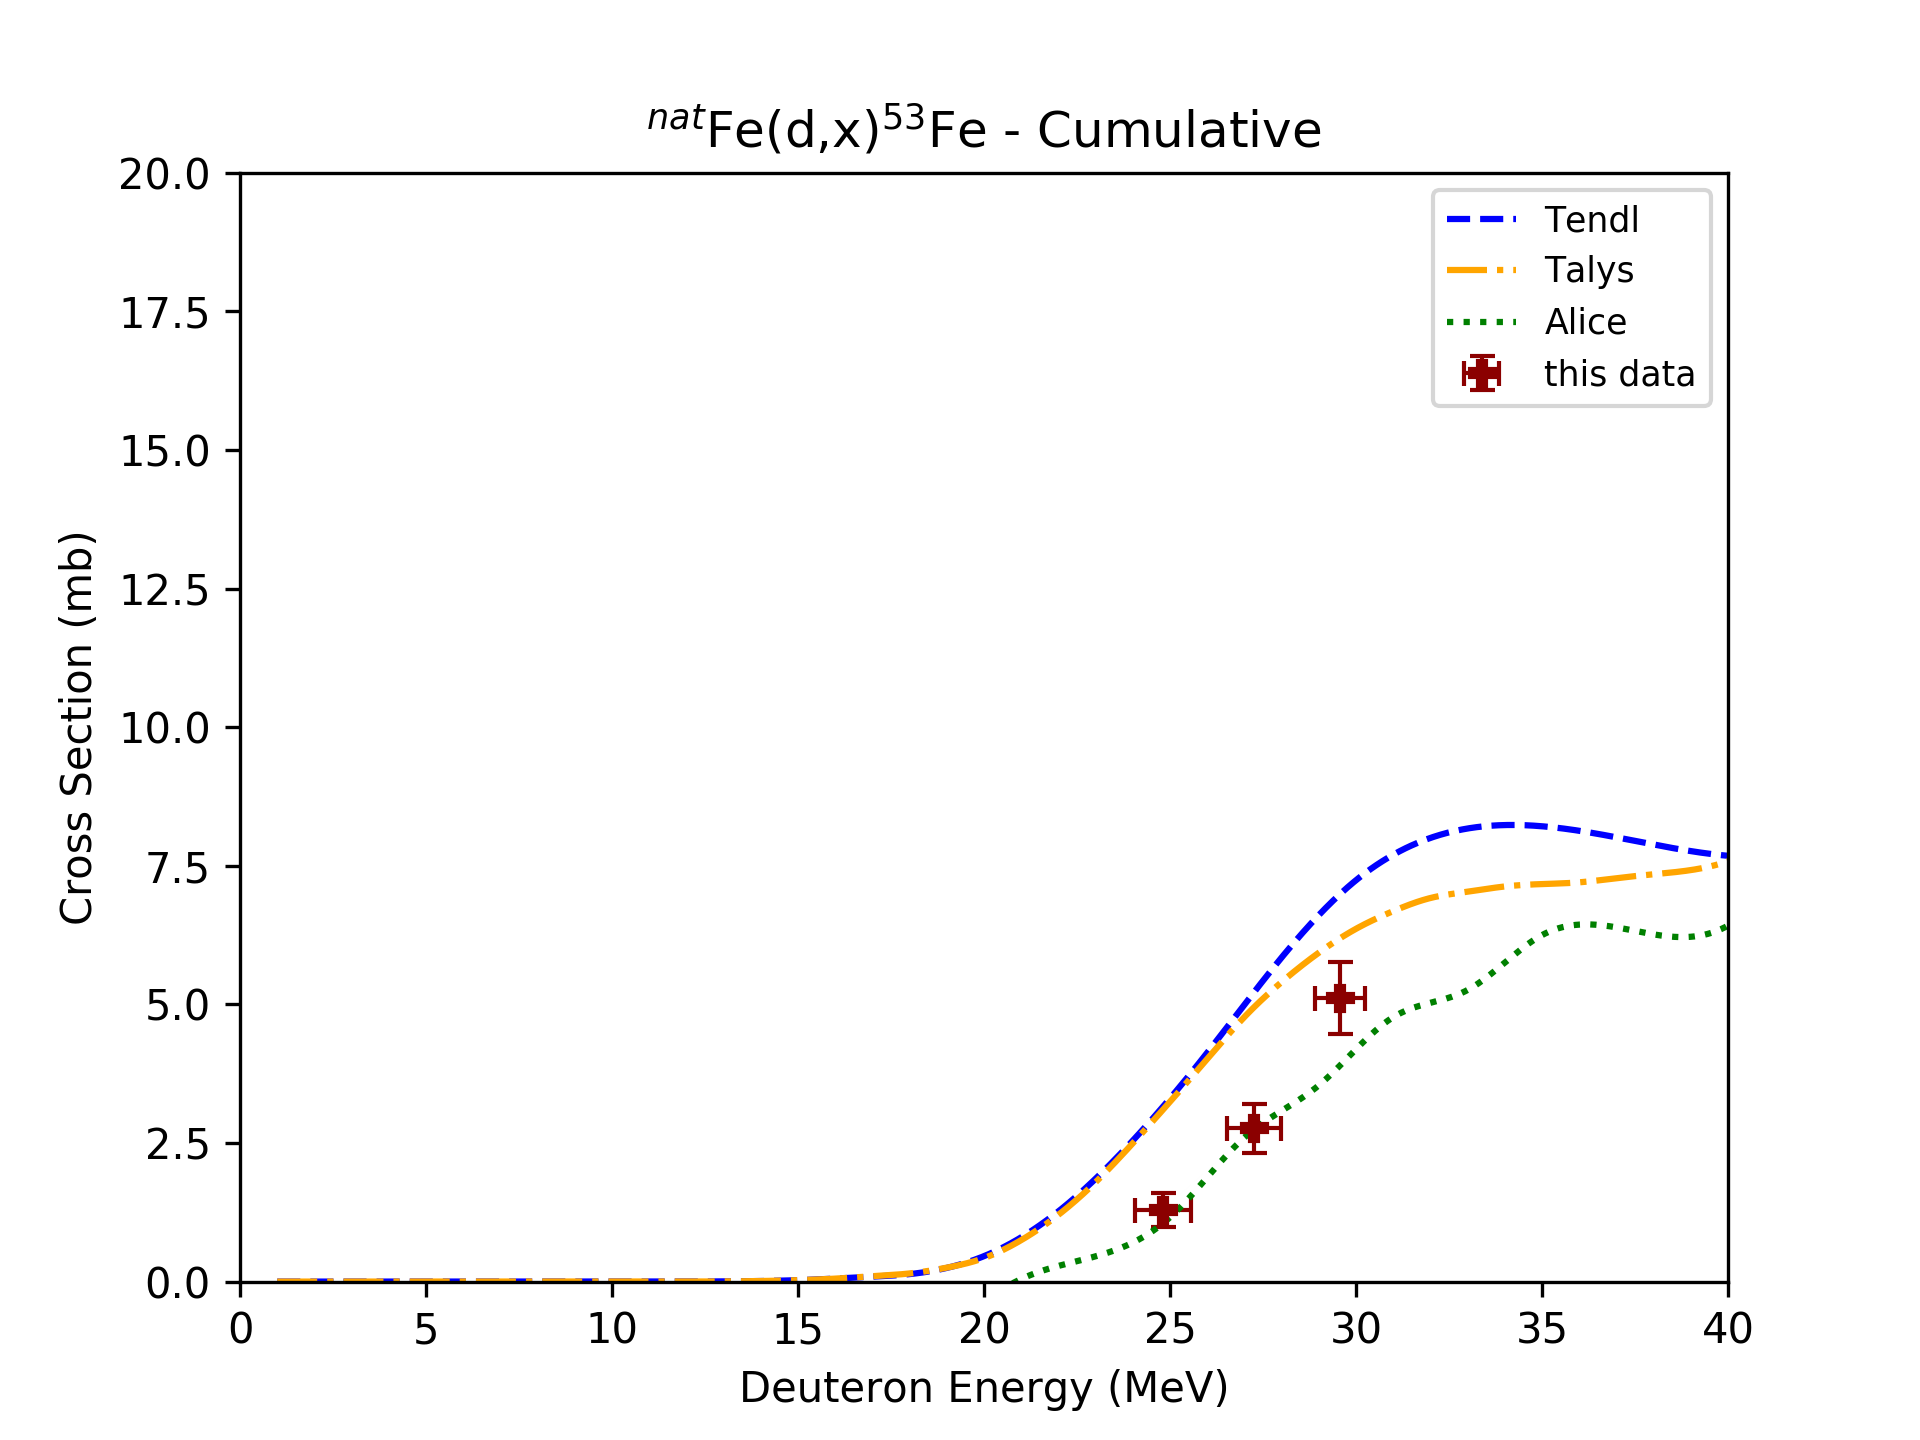
\includegraphics[width=5cm]{Results/Fe_53Fe.png} }}%
    \quad
    \subfloat[]{{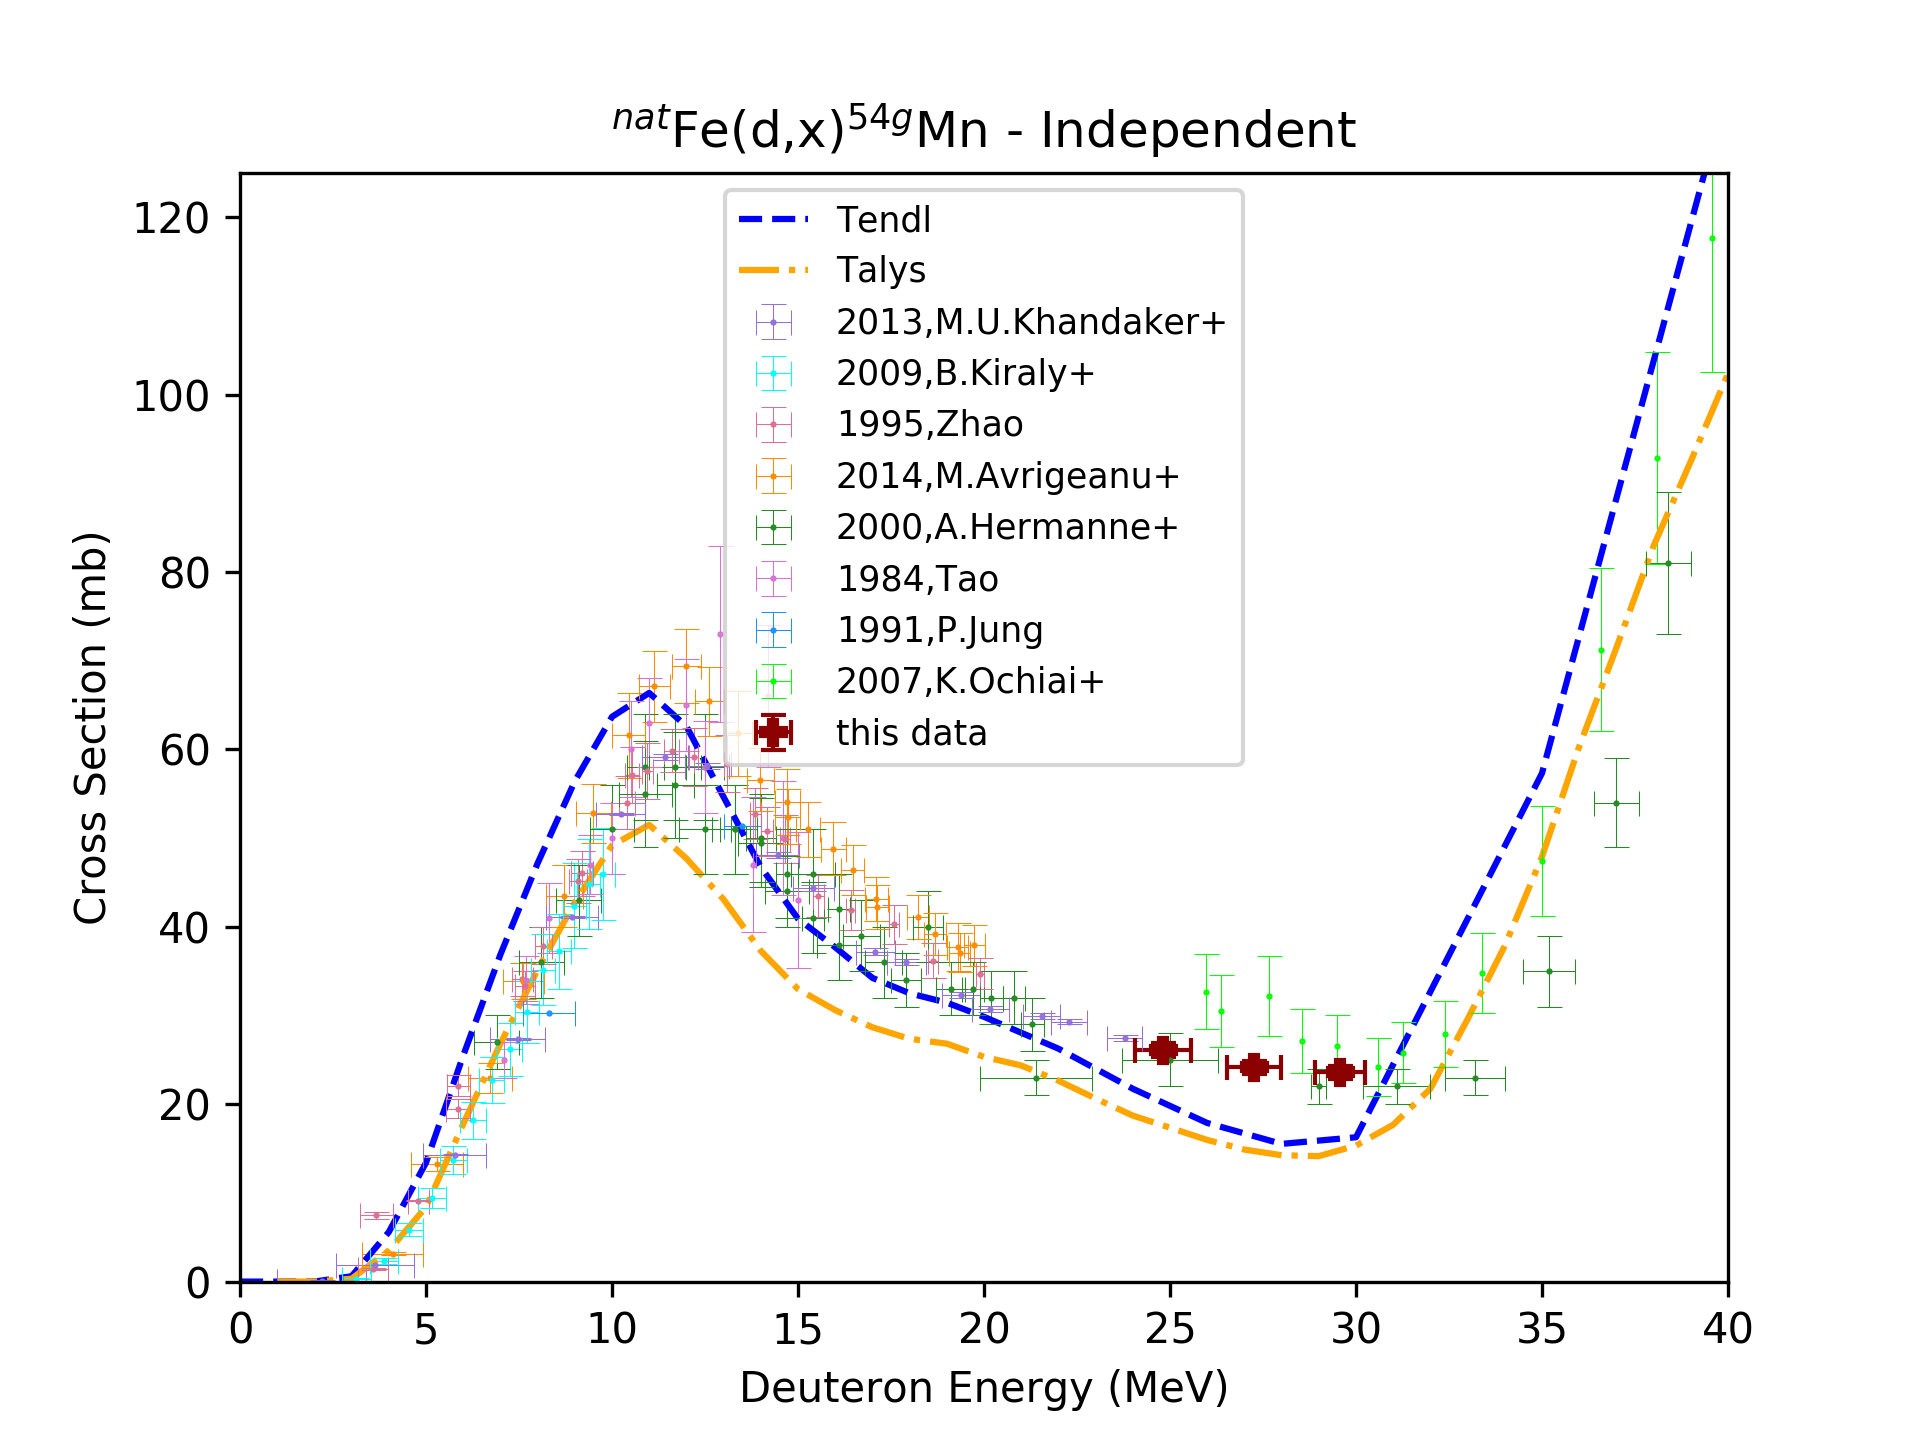
\includegraphics[width=5cm]{Results/Fe_54Mn.png} }}%
    \quad
    \subfloat[caption]{{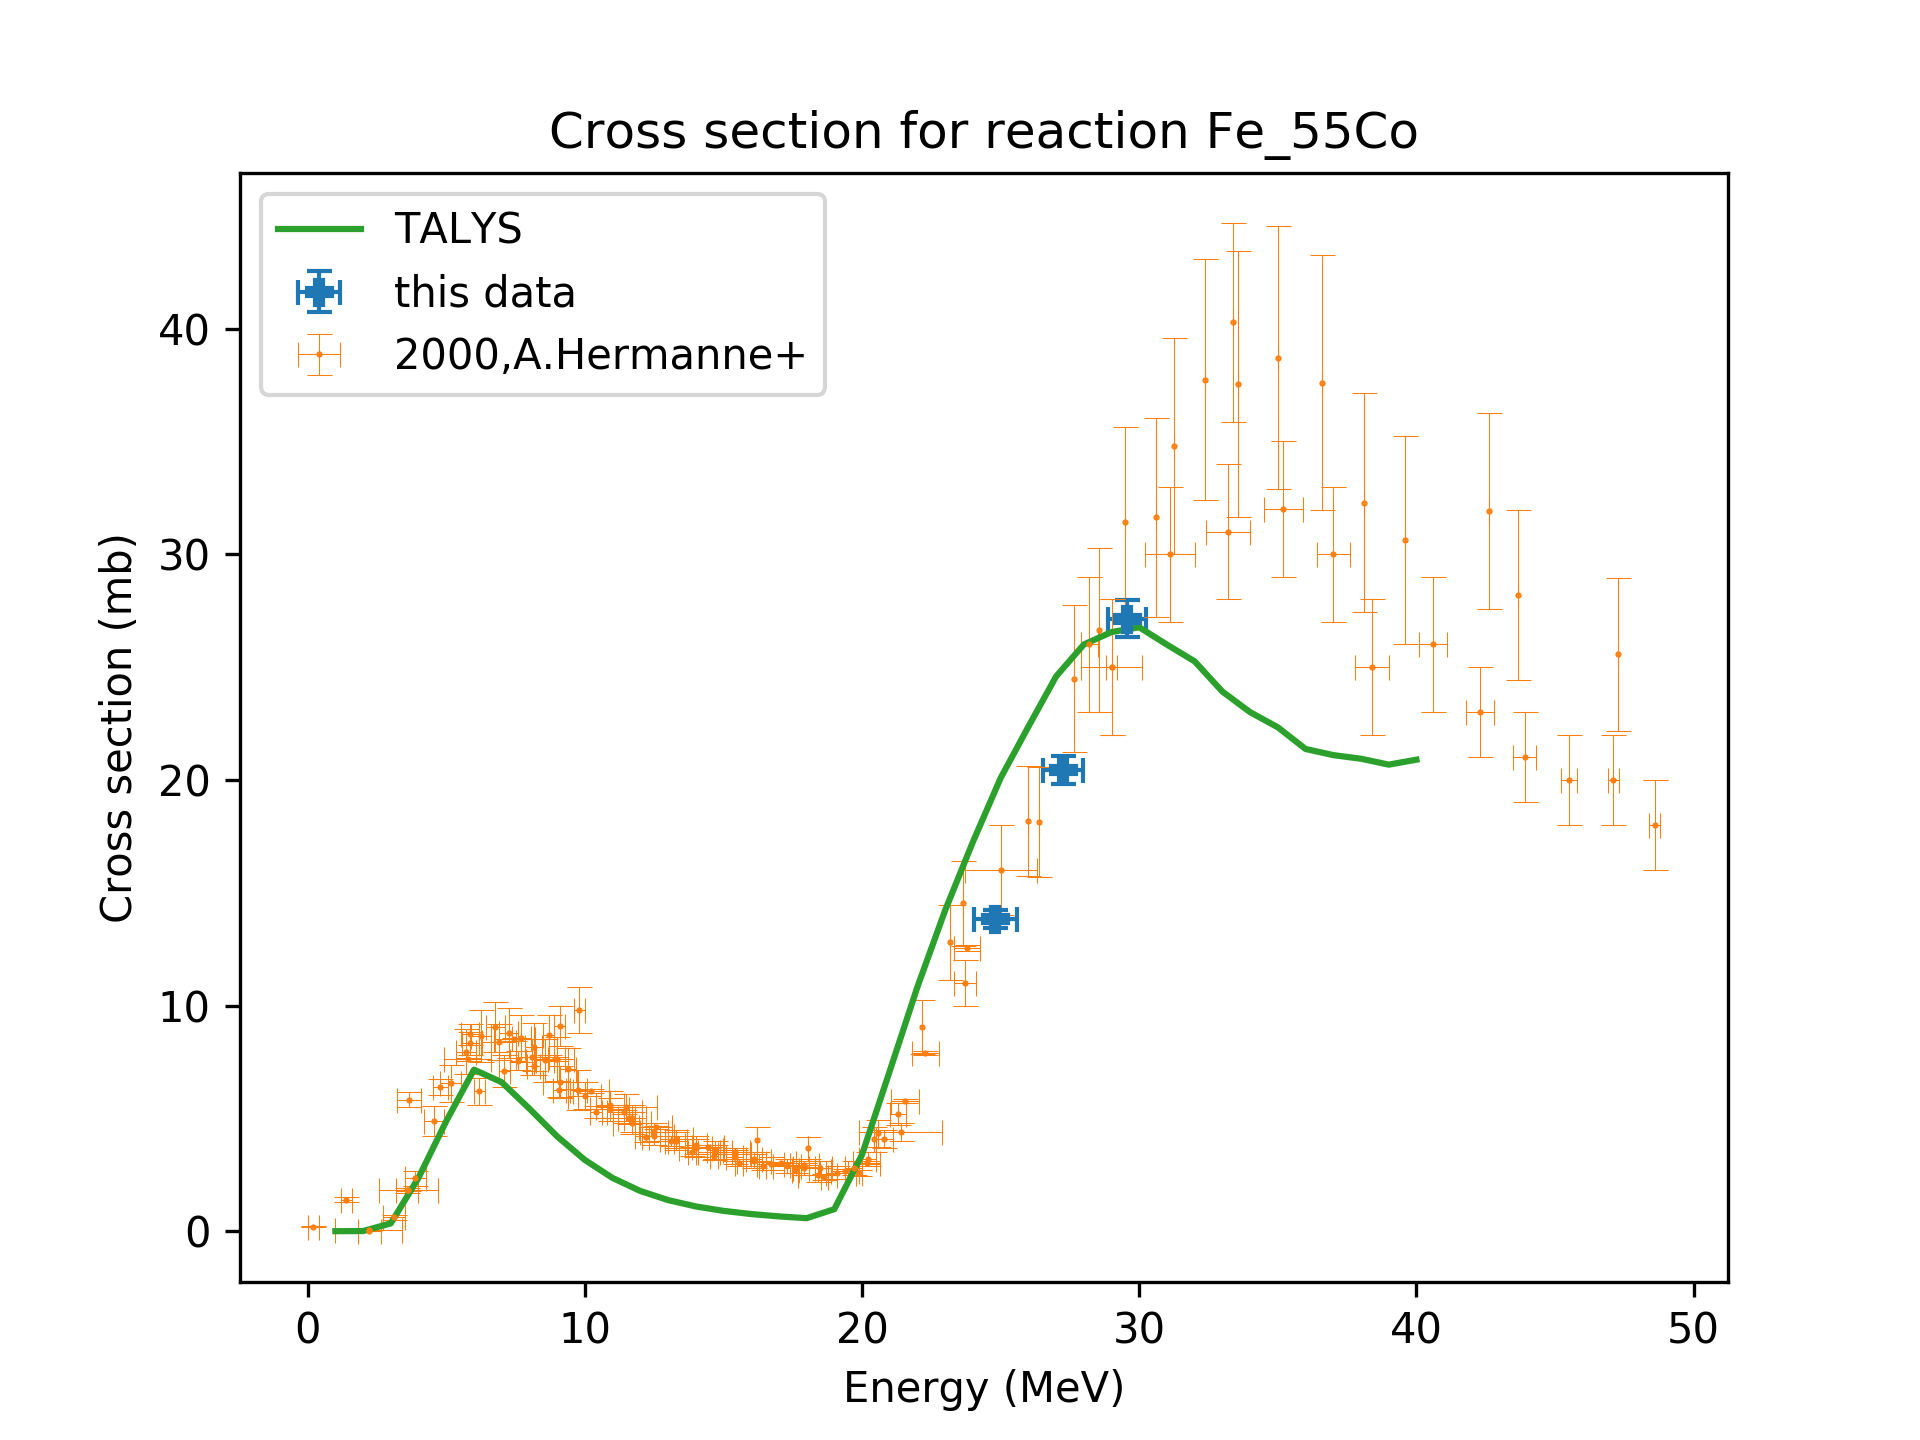
\includegraphics[width=5cm]{Results/Fe_55Co.png} }}%
    \quad
    \subfloat[caption]{{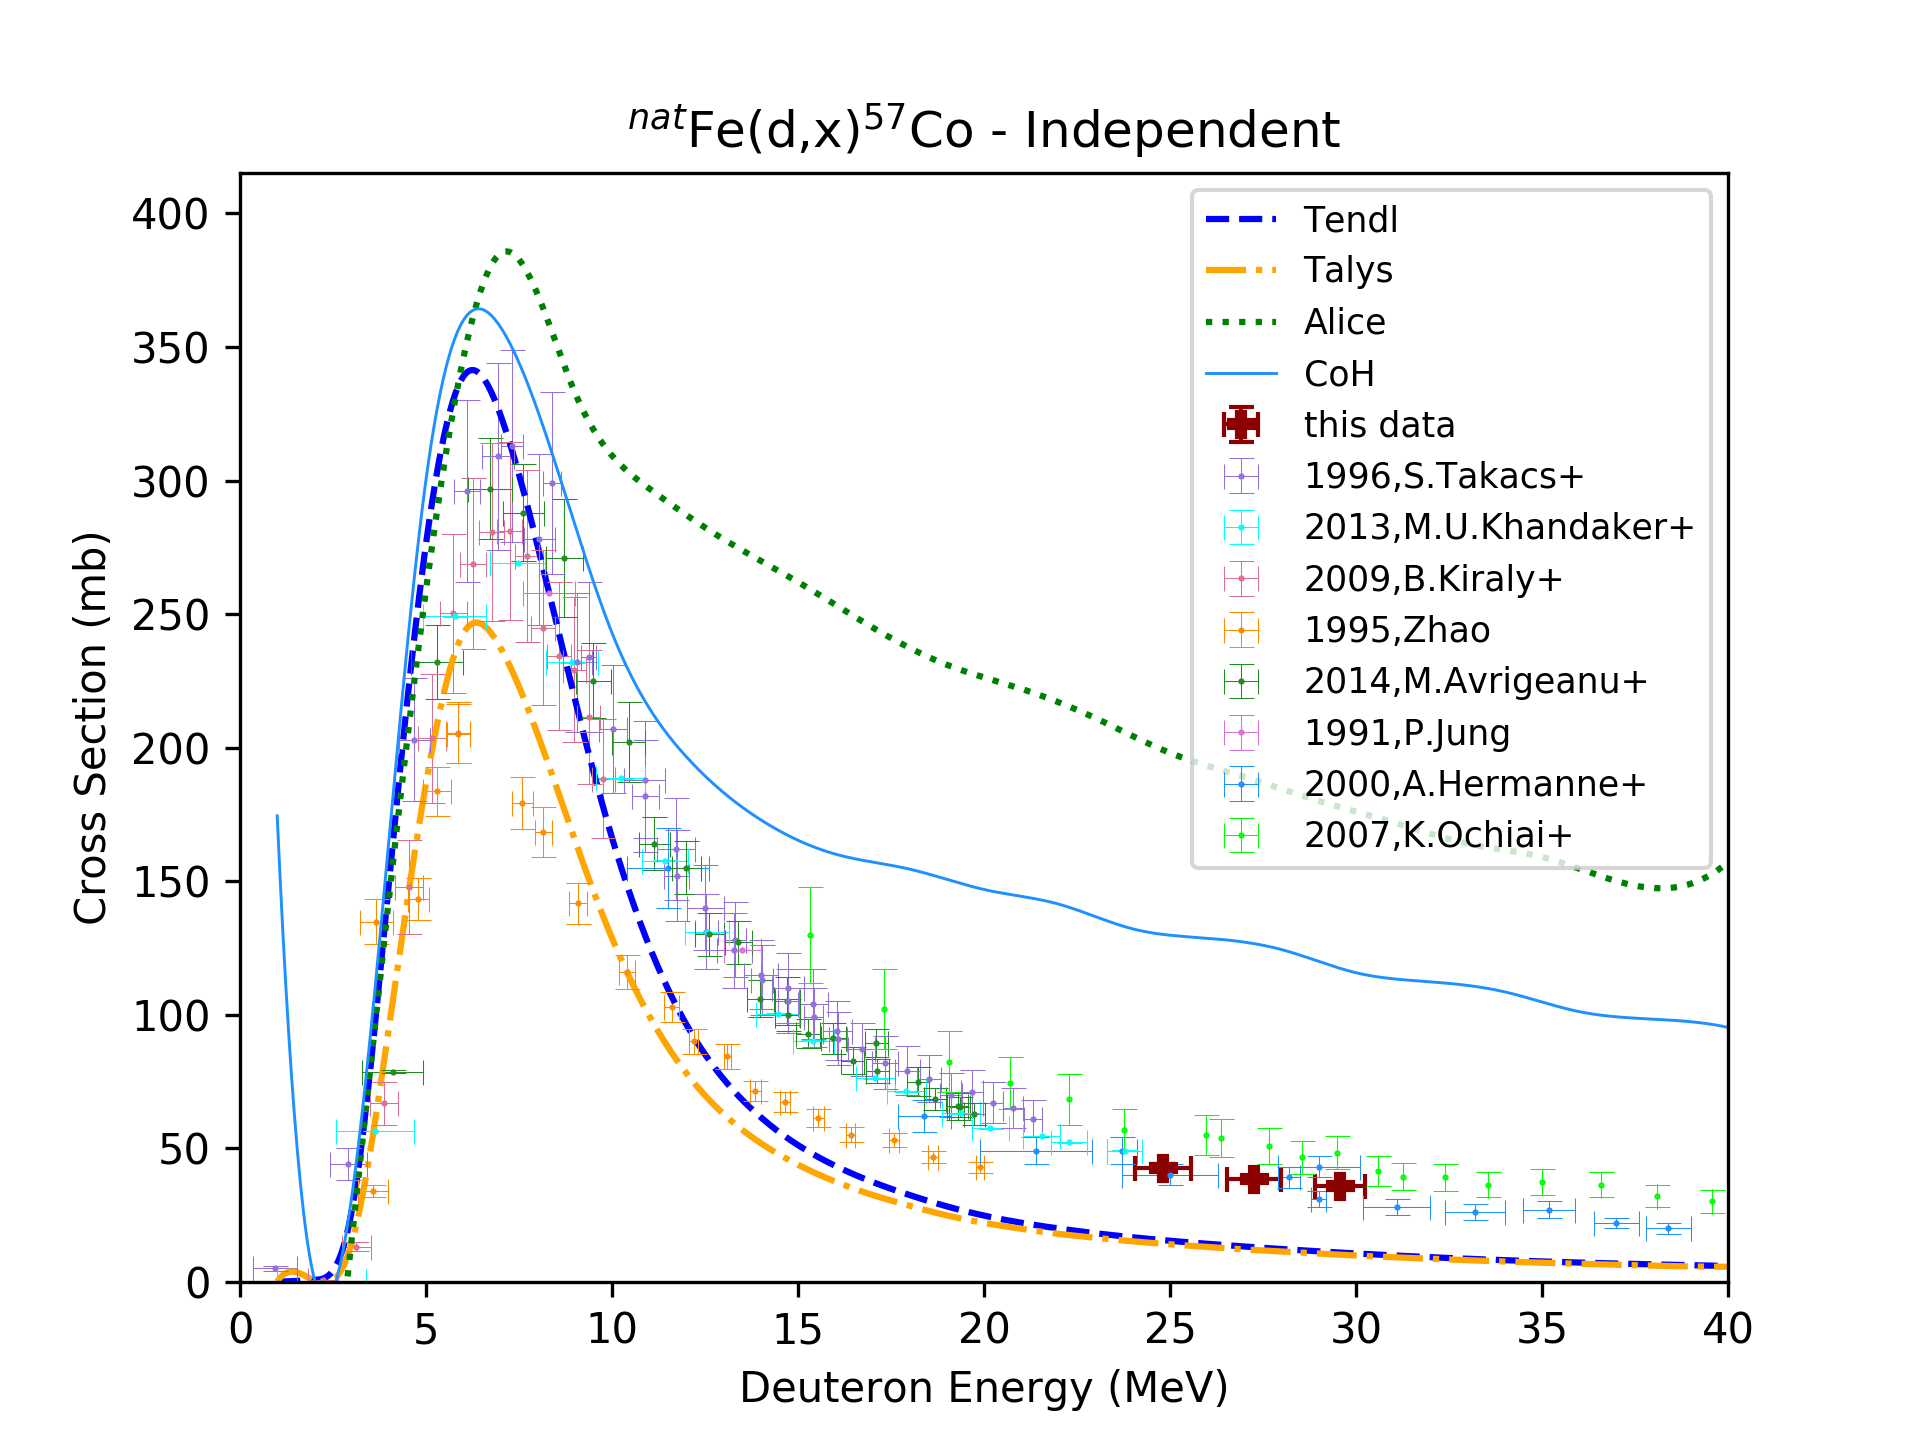
\includegraphics[width=5cm]{Results/Fe_57Co.png} }}%
    \quad
    \subfloat[caption]{{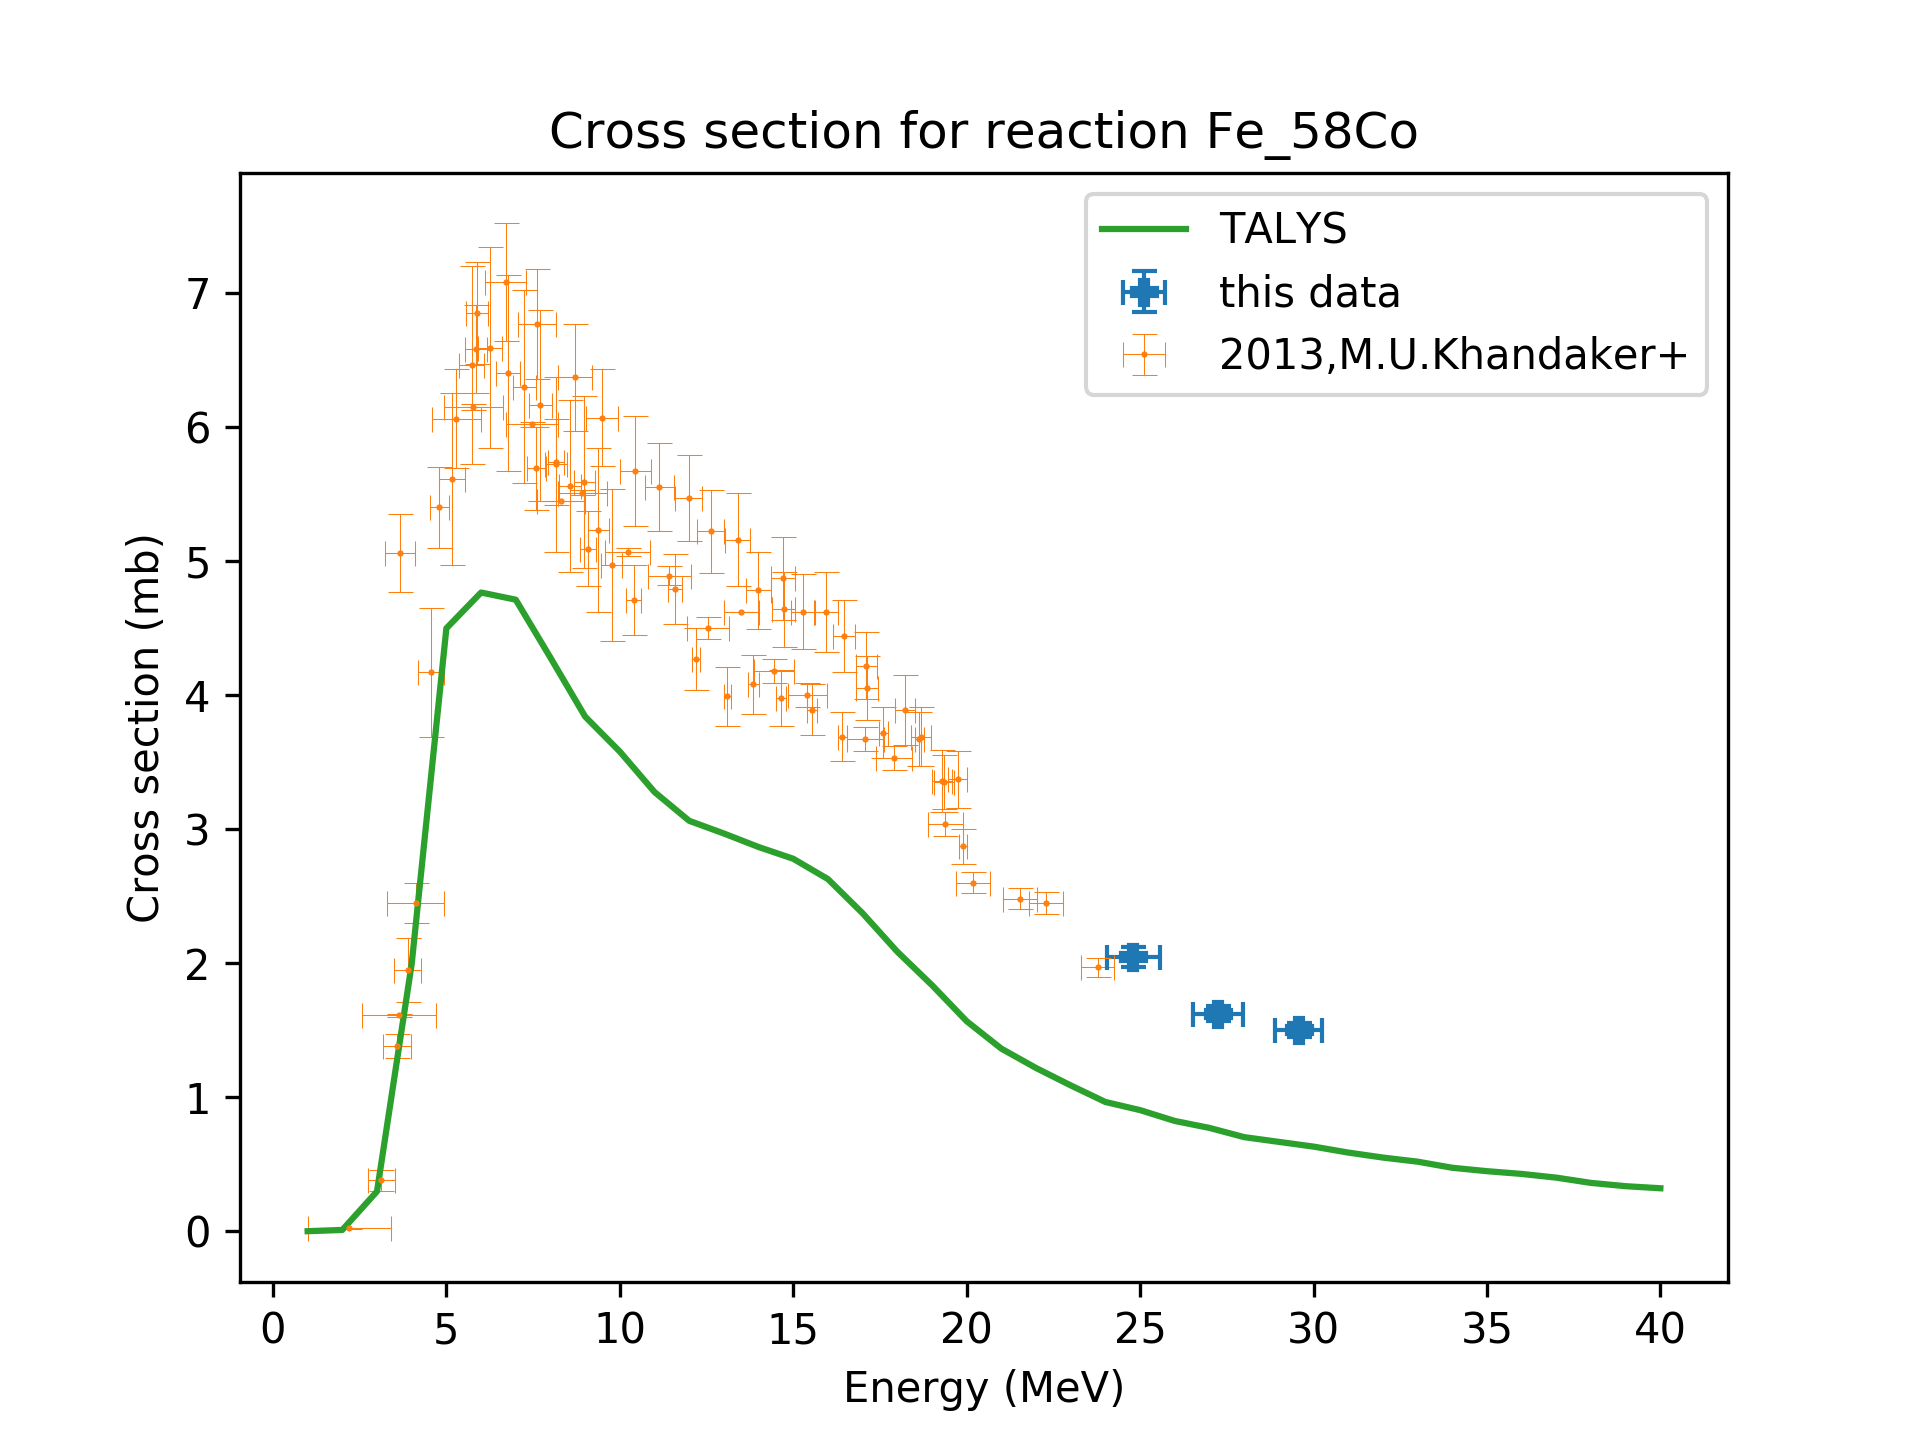
\includegraphics[width=5cm]{Results/Fe_58Co.png} }}%
    \quad
    \subfloat[caption]{{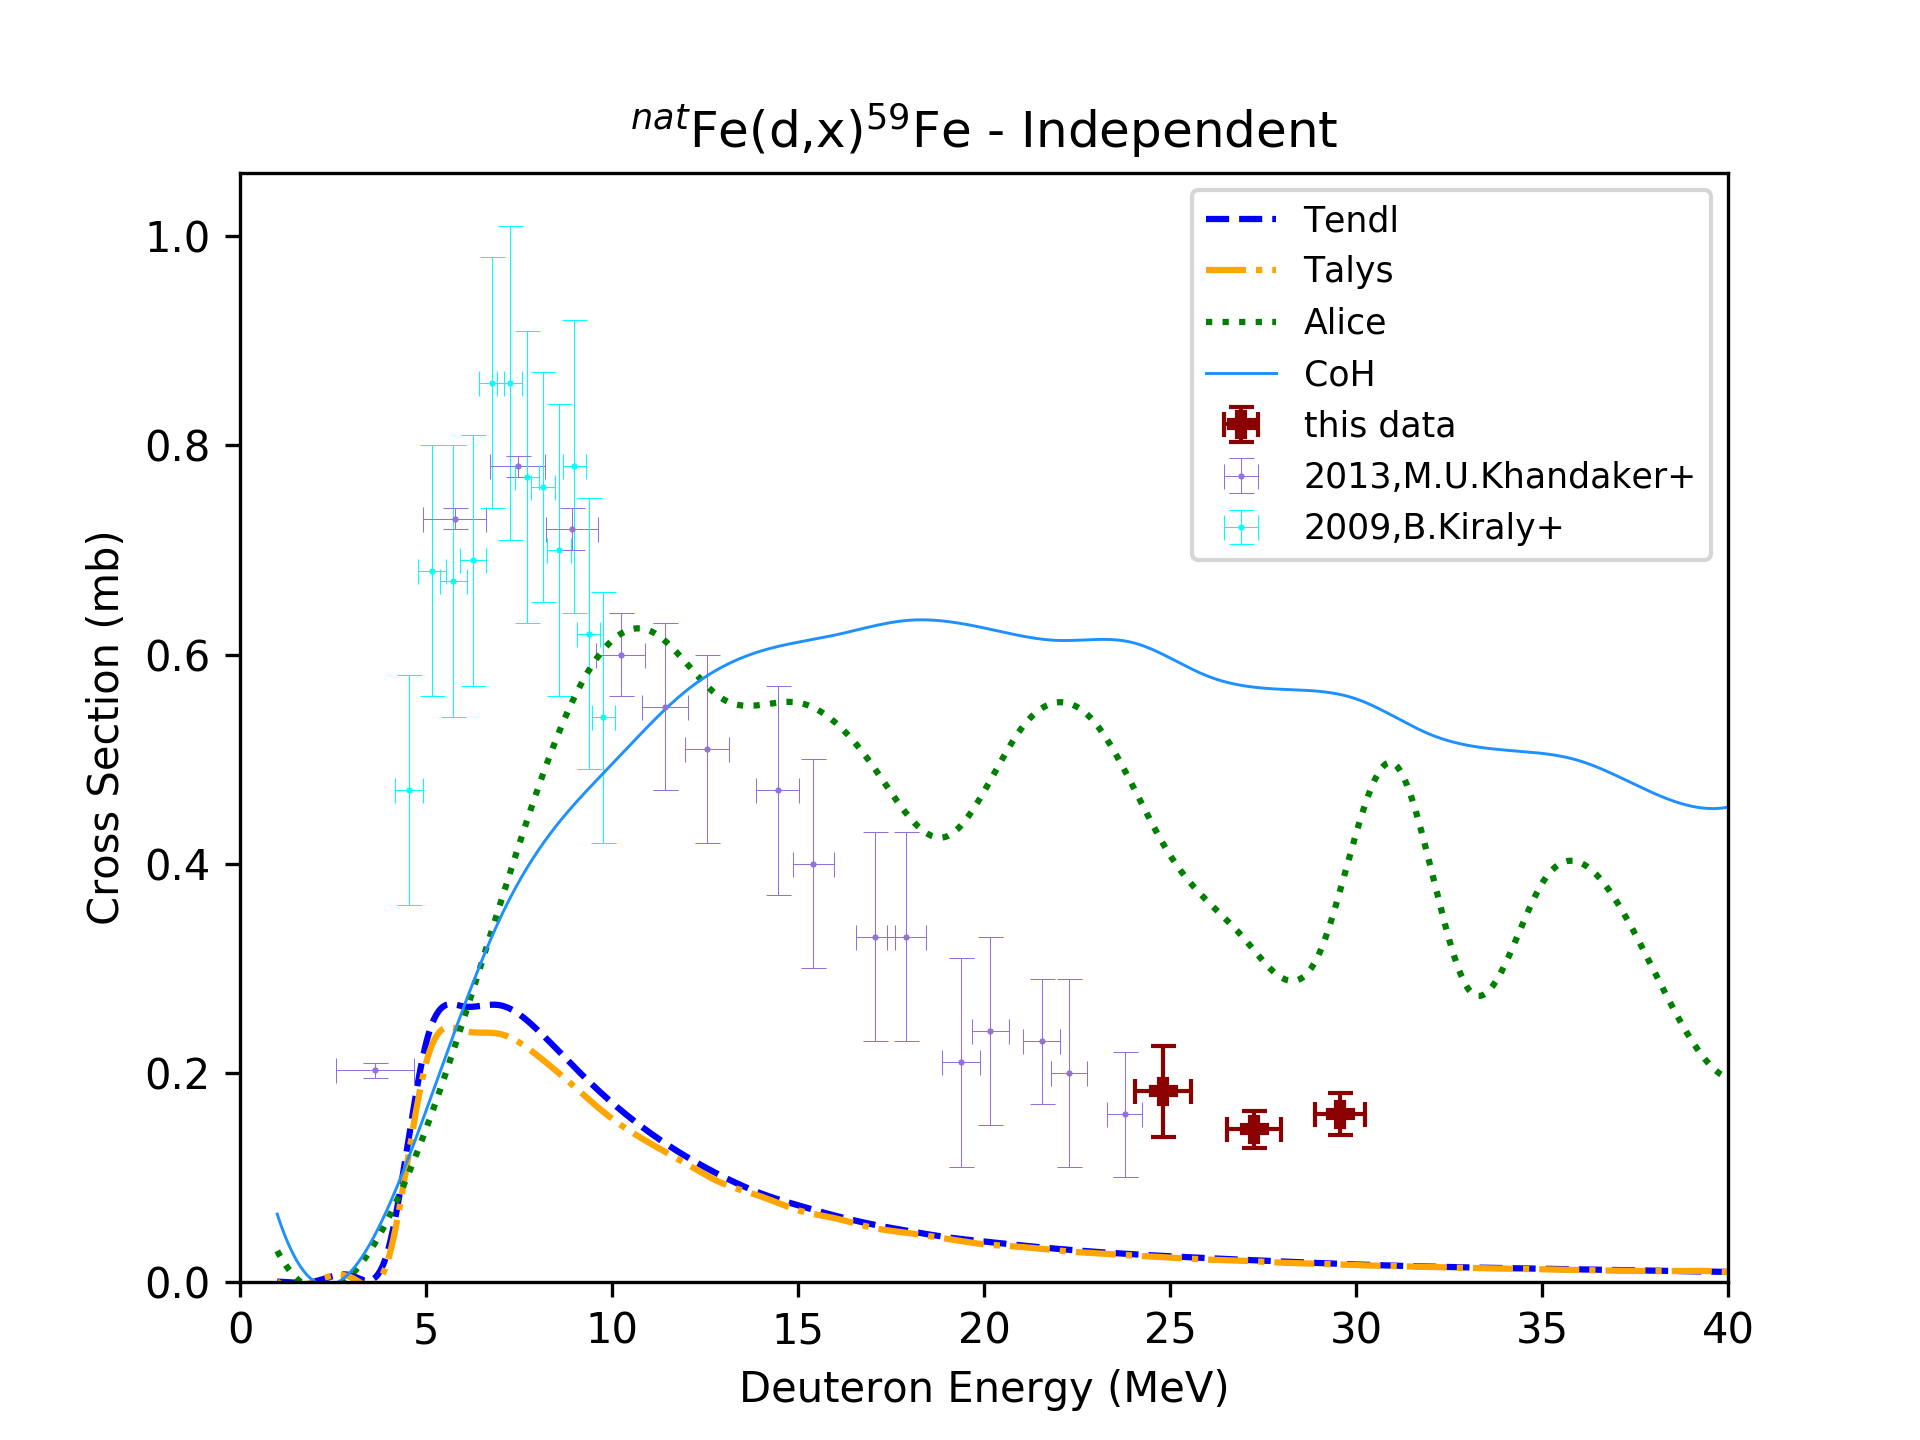
\includegraphics[width=5cm]{Results/Fe_59Fe.png} }}%
    \quad
    \caption{Iron cross sections  }%
    \label{fig:Fe_crosssections}%
\end{figure}